\documentclass[12pt,openright,twoside,a4paper,english,french,spanish]{abntex2}

\usepackage{cmap}	
\usepackage{lmodern}	
\usepackage[T1]{fontenc}	
\usepackage[utf8]{inputenc}		
\usepackage{lastpage}		
\usepackage{indentfirst}
\usepackage{color}	
\usepackage{graphicx}	
\usepackage{units}
\usepackage[brazilian,hyperpageref]{backref}
\usepackage[alf]{abntex2cite}
\usepackage{bold-extra}
\usepackage{eso-pic}

\renewcommand{\backrefpagesname}{Citado na(s) página(s):~}
\renewcommand{\backref}{}
\renewcommand*{\backrefalt}[4]{
	\ifcase #1 %
		Nenhuma citação no texto.%
	\or
		Citado na página #2.%
	\else
		Citado #1 vezes nas páginas #2.%
	\fi}%
% ---


\newcommand{\curso}[1]{\def\imprimircurso{#1}}

\newcommand{\palavraChaveUm}[1]{\def\imprimirpalavrachaveum{#1}}
\newcommand{\palavraChaveDois}[1]{\def\imprimirpalavrachavedois{#1}}
\newcommand{\palavraChaveTres}[1]{\def\imprimirpalavrachavetres{#1}}
\newcommand{\palavraChaveQuatro}[1]{\def\imprimirpalavrachavequatro{#1}}
\newcommand{\palavraChaveCinco}[1]{\def\imprimirpalavrachavecinco{#1}}

\newcommand{\cdu}[1]{\def\nomecdu{#1}}
\newcommand{\dataDaAprovacao}[1]{\def\imprimirdatadaaprovacao{#1}}

\newcommand{\membroConvidadoUm}[1]{\def\imprimirmembroconvidadoum{#1}}
\newcommand{\membroConvidadoDois}[1]{\def\imprimirmembroconvidadodois{#1}}

\newcommand\BackgroundPic{%
	\put(0,0){%
		\parbox[b][\paperheight]{\paperwidth}{%
			\vfill
			\centering
			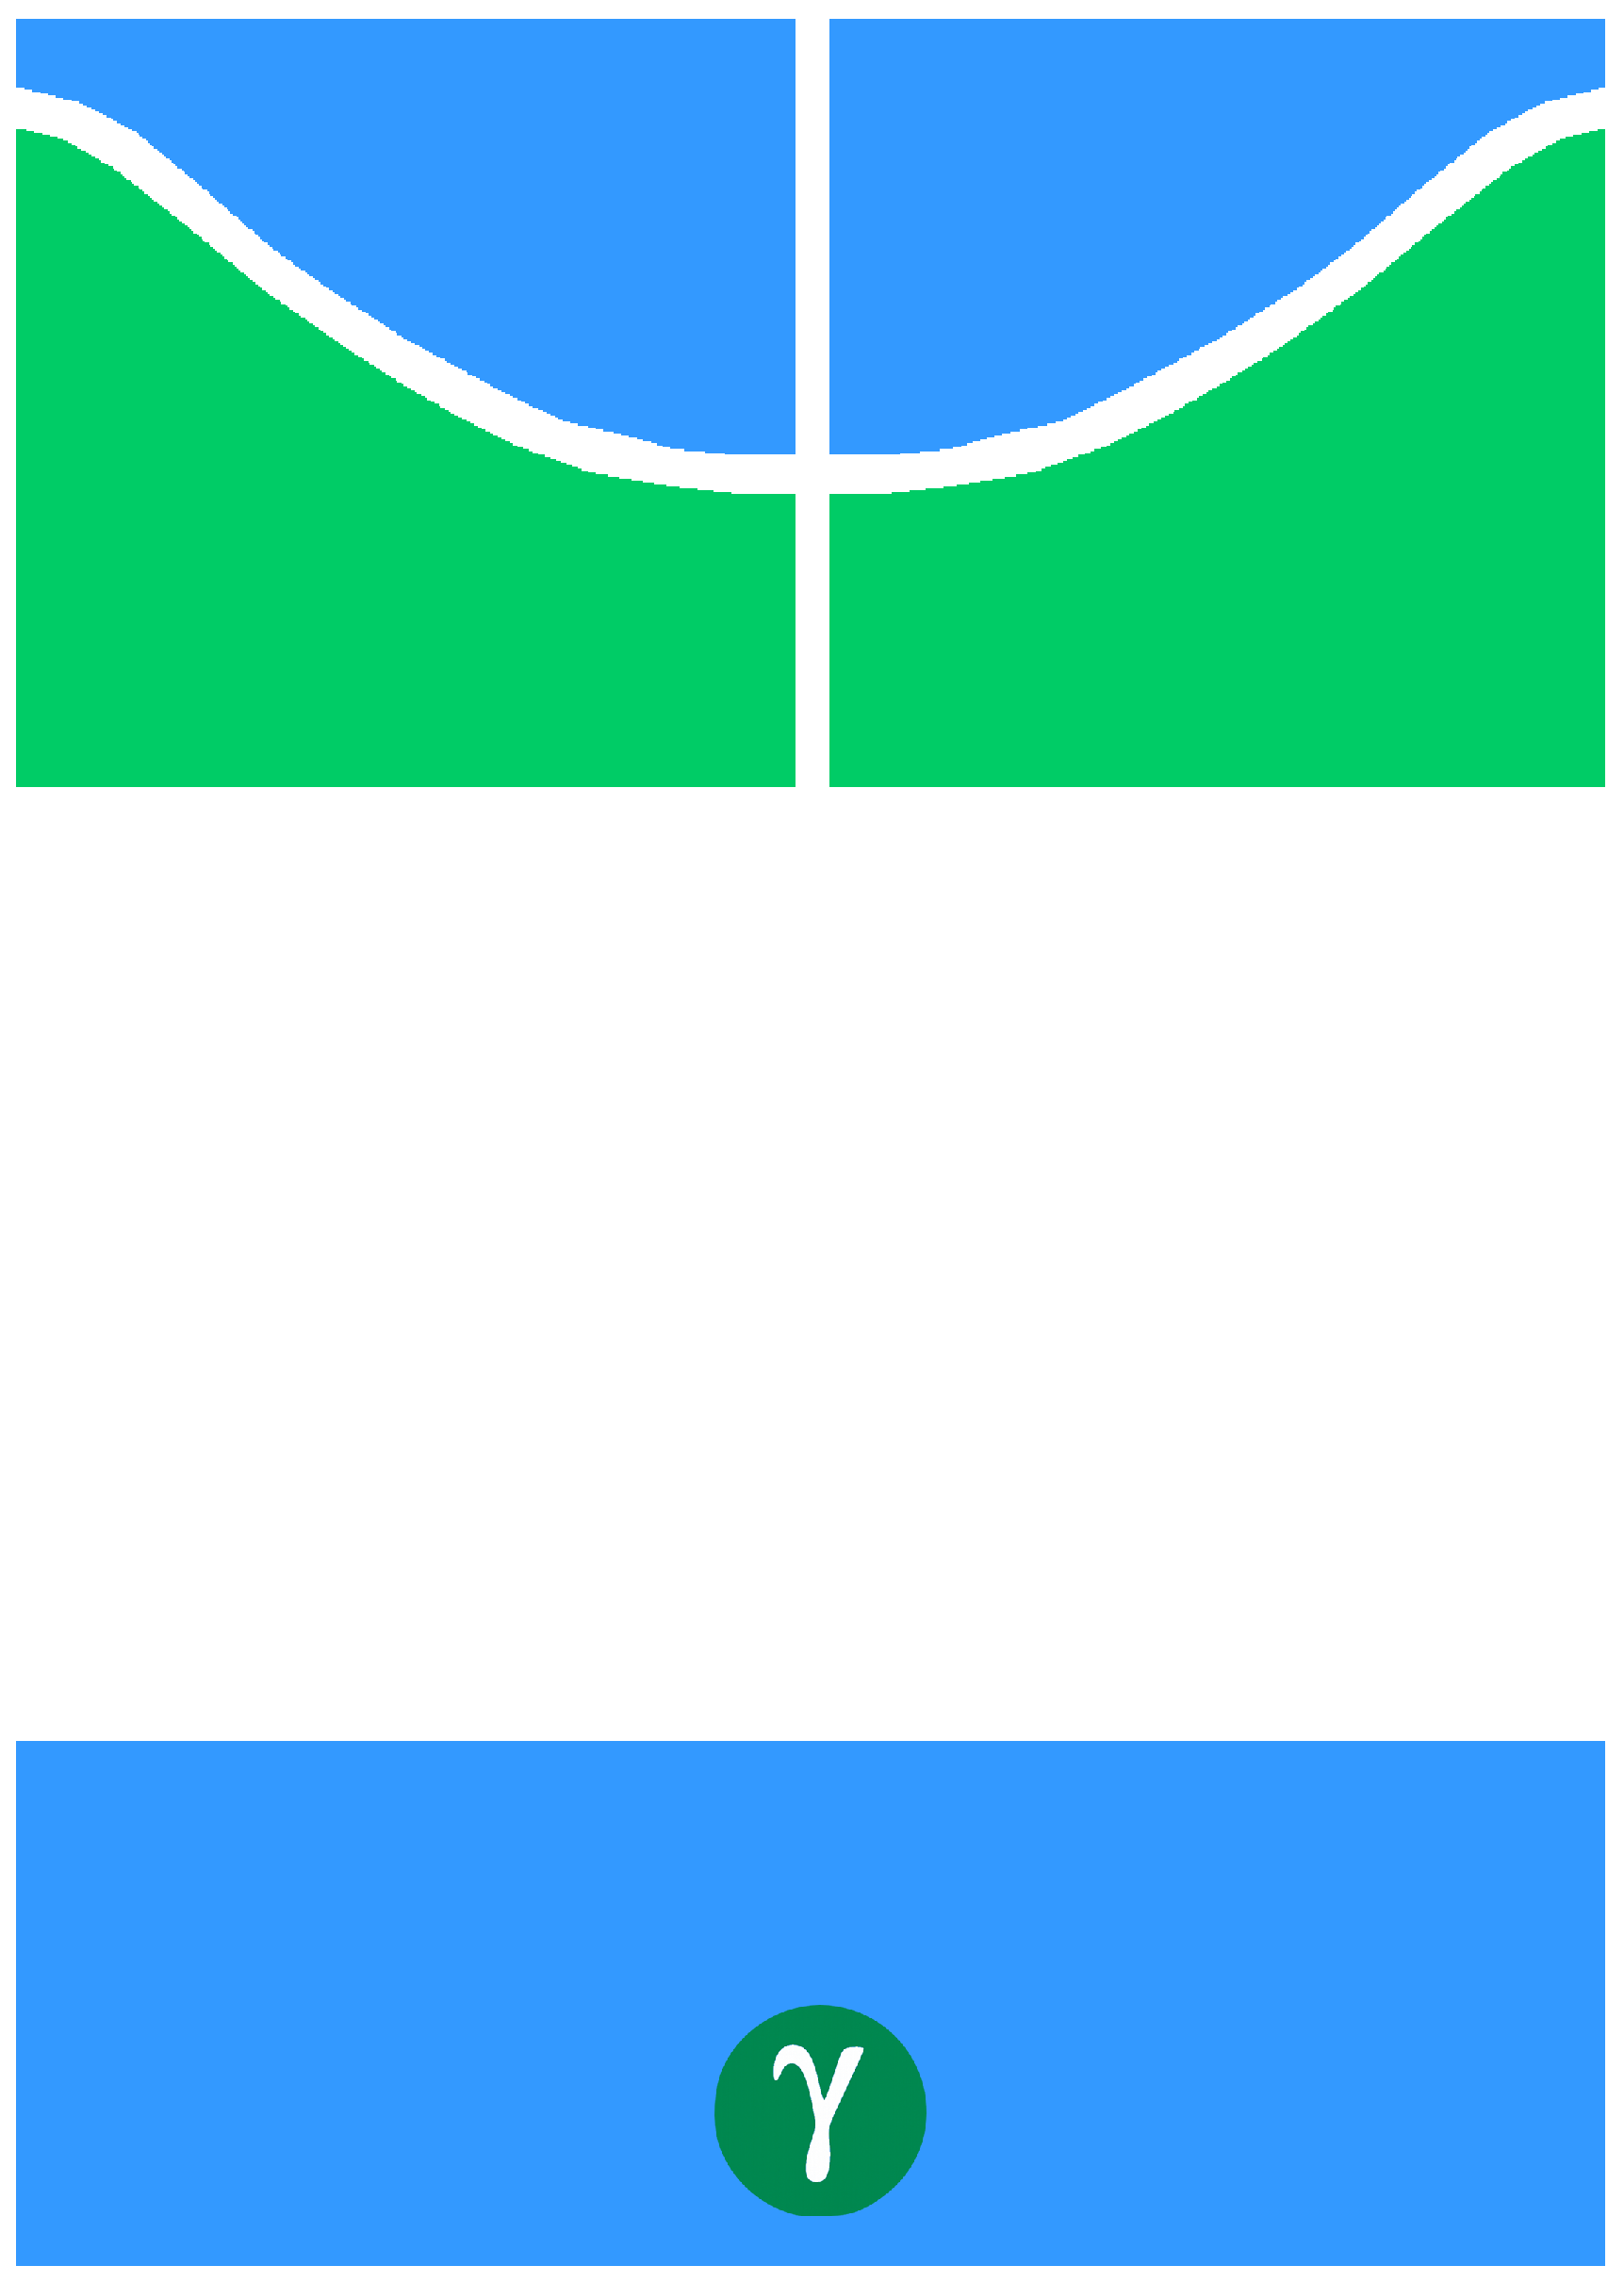
\includegraphics[width=\paperwidth,height=\paperheight,%
				keepaspectratio]{figuras/capa.eps}%
			\vfill
		}
	}
}

\renewcommand{\imprimircapa}{%
  \begin{capa}%
    \center
	\AddToShipoutPicture*{\BackgroundPic}

%	\begin{huge}
%		\textbf{\textsc{Trabalho de Conclusão de Curso}}
%	\end{huge}

    \vspace*{2.7in}
	{\textbf{\large\imprimirinstituicao}}
	\par
	{\textbf{\large\imprimircurso}}

	\vspace{0.5in}

    {\ABNTEXchapterfont\bfseries\LARGE\imprimirtitulo}
    \vspace*{\fill}

	\begin{flushright}
    	\textbf{{\large{Autor: \imprimirautor}}}
		\par
    	\textbf{{\large{Orientador: \imprimirorientador}}}
	\end{flushright}

    \vspace*{0.2in}
    \textbf{{\large\imprimirlocal}}
    \par
    \textbf{{\large\imprimirdata}}

    \vspace*{2.2in}
  \end{capa}
}



% Dados pessoais
\autor{Nome do Autor}
\curso{Nome do Curso}

% Dados do trabalho
\titulo{Título: Subtítulo do Trabalho}
\data{2013}
\palavraChaveUm{Palavra-chave01}
\palavraChaveDois{Palavra-chave02}

% Dados da orientacao
\orientador{(Titulação Acadêmica e Nome do Orientador)}
\coorientador{(quando houver, Titulação Acadêmica e Nome do Orientador)}

% Dados para a ficha catalográfica
\cdu{02:141:005.6}

% Dados da aprovação do trabalho
\dataDaAprovacao{01 de junho de 2013}
\membroConvidadoUm{Titulação e Nome do Professor Convidado 01}
\membroConvidadoDois{Titulação e Nome do Professor Convidado 02}

\local{Brasília, DF}
\instituicao{%
  Universidade de Brasília - UnB
  \par
  Faculdade UnB Gama - FGA
}
\tipotrabalho{Trabalho de Conclusão de Curso}
\preambulo{Monografia submetida ao curso de graduação em (\imprimircurso) 
da Universidade de Brasília, como requisito parcial para obtenção do Título 
de Bacharel em (\imprimircurso).}

\definecolor{blue}{RGB}{41,5,195}
\makeatletter
\hypersetup{
     	%pagebackref=true,
		pdftitle={\@title}, 
		pdfauthor={\@author},
    	pdfsubject={\imprimirpreambulo},
	    pdfcreator={LaTeX with abnTeX2},
		pdfkeywords={abnt}{latex}{abntex}{abntex2}{trabalho acadêmico}, 
		colorlinks=true,       		% false: boxed links; true: colored links
    	linkcolor=blue,          	% color of internal links
    	citecolor=blue,        		% color of links to bibliography
    	filecolor=magenta,      		% color of file links
		urlcolor=blue,
		bookmarksdepth=4
}
\makeatother
\setlength{\parindent}{1.3cm}
\setlength{\parskip}{0.2cm}  
\makeindex


\DeclareFixedFont{\ttb}{T1}{txtt}{bx}{n}{12} % for bold
\DeclareFixedFont{\ttm}{T1}{txtt}{m}{n}{12}  % for normal
\definecolor{deepblue}{rgb}{0,0,0.5}
\definecolor{deepred}{rgb}{0.6,0,0}
\definecolor{deepgreen}{rgb}{0,0.5,0}

\usepackage{listings}

\newcommand\pythonstyle{\lstset{
language=Python,
basicstyle=\ttm,
otherkeywords={self},             % Add keywords here
keywordstyle=\ttb\color{deepblue},
emph={MyClass,__init__},          % Custom highlighting
emphstyle=\ttb\color{deepred},    % Custom highlighting style
stringstyle=\color{deepgreen},
frame=tb,                         % Any extra options here
showstringspaces=false            %
}}

% Python environment
\lstnewenvironment{python}[1][]
{
\pythonstyle
\lstset{#1}
}
{}

% Python for external files
\newcommand\pythonexternal[2][]{{
\pythonstyle
\lstinputlisting[#1]{#2}}}

% Python for inline
\newcommand\pythoninline[1]{{\pythonstyle\lstinline!#1!}}

\renewcommand{\lstlistingname}{Algoritmo}% Listing -> Algorithm
\renewcommand{\lstlistlistingname}{Lista de \lstlistingname s}% List of Listings -> List of Algorithms

\begin{document}

\frenchspacing
\imprimircapa
\imprimirfolhaderosto*

\begin{fichacatalografica}
	\vspace*{\fill}					% Posição vertical
	\hrule							% Linha horizontal
	\begin{center}					% Minipage Centralizado
	\begin{minipage}[c]{12.5cm}		% Largura
	
	\imprimirautor
	
	\hspace{0.5cm} \imprimirtitulo  / \imprimirautor. --
	\imprimirlocal, \imprimirdata-
	
	\hspace{0.5cm} \pageref{LastPage} p. : il. (algumas color.) ; 30 cm.\\
	
	\hspace{0.5cm} \imprimirorientadorRotulo~\imprimirorientador\\
	
	\hspace{0.5cm}
	\parbox[t]{\textwidth}{\imprimirtipotrabalho~--~\imprimirinstituicao,
	\imprimirdata.}\\
	
	\hspace{0.5cm}
		1. \imprimirpalavrachaveum.
		2. \imprimirpalavrachavedois.
		I. \imprimirorientador.
		II. Universidade de Brasília.
		III. Faculdade UnB Gama.
		IV. \imprimirtitulo\\ 			
	
	\hspace{8.75cm} CDU \nomecdu\\
	
	\end{minipage}
	\end{center}
	\hrule
\end{fichacatalografica}

\begin{errata}
Elemento opcional da \citeonline[4.2.1.2]{NBR14724:2011}. \textbf{Caso não 
deseje uma errata, deixar todo este arquivo em branco}. Exemplo:

\vspace{\onelineskip}

FERRIGNO, C. R. A. \textbf{Tratamento de neoplasias ósseas apendiculares com
reimplantação de enxerto ósseo autólogo autoclavado associado ao plasma
rico em plaquetas}: estudo crítico na cirurgia de preservação de membro em
cães. 2011. 128 f. Tese (Livre-Docência) - Faculdade de Medicina Veterinária e
Zootecnia, Universidade de São Paulo, São Paulo, 2011.

\begin{table}[htb]
\center
\footnotesize
\begin{tabular}{|p{1.4cm}|p{1cm}|p{3cm}|p{3cm}|}
  \hline
   \textbf{Folha} & \textbf{Linha}  & \textbf{Onde se lê}  & \textbf{Leia-se}  \\
    \hline
    1 & 10 & auto-conclavo & autoconclavo\\
   \hline
\end{tabular}
\end{table}

\end{errata}

\begin{folhadeaprovacao}

  \begin{center}
    {\ABNTEXchapterfont\large\imprimirautor}

    \vspace*{\fill}\vspace*{\fill}
    {\ABNTEXchapterfont\bfseries\Large\imprimirtitulo}
    \vspace*{\fill}
    
    \hspace{.45\textwidth}
    \begin{minipage}{.5\textwidth}
        \imprimirpreambulo
    \end{minipage}%
    \vspace*{\fill}
   \end{center}
    
   Trabalho aprovado. \imprimirlocal, \imprimirdatadaaprovacao:

   \assinatura{\textbf{\imprimirorientador} \\ Orientador} 
   \assinatura{\textbf{\imprimirmembroconvidadoum} \\ Convidado 1}
   \assinatura{\textbf{\imprimirmembroconvidadodois} \\ Convidado 2}
      
   \begin{center}
    \vspace*{0.5cm}
    {\large\imprimirlocal}
    \par
    {\large\imprimirdata}
    \vspace*{1cm}
  \end{center}
  
\end{folhadeaprovacao}

%\begin{dedicatoria}
   \vspace*{\fill}
   \centering
   \noindent
	\textbf{A dedicatória é opcional. Caso não deseje uma, deixar todo este
	arquivo em branco}.

   \textit{Este trabalho é dedicado às crianças adultas que,\\
   quando pequenas, sonharam em se tornar cientistas.} \vspace*{\fill}
\end{dedicatoria}

%\begin{agradecimentos}
A inclusão desta seção de agradecimentos é opcional, portanto, sua inclusão 
fica a critério do(s) autor(es), que caso deseje(em) fazê-lo deverá(ão) 
utilizar este espaço, seguindo a formatação de \textit{espaço simples e 
fonte padrão do texto (arial ou times, tamanho 12 sem negritos, aspas ou 
itálico}.

\textbf{Caso não deseje utilizar os agradecimentos, deixar toda este arquivo
em branco}.
\end{agradecimentos}

%\begin{epigrafe}
    \vspace*{\fill}
	\begin{flushright}
		\textbf{A epígrafe é opcional. Caso não deseje uma, deixe todo
		este arquivo em branco}.

		\textit{``Não vos amoldeis às estruturas deste mundo, \\
		mas transformai-vos pela renovação da mente, \\
		a fim de distinguir qual é a vontade de Deus: \\
		o que é bom, o que Lhe é agradável, o que é perfeito.\\
		(Bíblia Sagrada, Romanos 12, 2)}
	\end{flushright}
\end{epigrafe}

\begin{resumo}
O consumo enérgico irracional vem crescendo com o passar dos anos. Os órgãos públicos deveriam dar o exemplo à população, tendo um consumo mais consciente, porém, muitos órgãos brasileiros ainda não possuem nenhum projeto que visa suas eficiências energéticas. A Universidade de Brasília, passando por esse problema, decidiu realizar um investimento para essas questões, objetivando um monitoramento energético adequado para seus câmpus. Com esse monitoramento sendo realizado de maneira efetiva, seria possível a realização de possíveis políticas para a redução do consumo de energia. O objetivo deste trabalho é utilizar os conhecimentos e métodos da Engenharia de Software, aplicando-os durante o desenvolvimento de um sistema \textit{web} para monitoramento de insumos, visando inicialmente os dados energéticos, da Universidade de Brasília. Os conceitos utilizados abordam práticas de desenvolvimento ágeis, software livre, gerência de configuração de software e tecnologias \textit{web}. Este trabalho apresenta como foi o ciclo de vida do sistema e detalhadamente todas as suas características importantes.

 \vspace{\onelineskip}

 \noindent
 \textbf{Palavras-chaves}: Engenharia de Software. Gerência de Configuração de Software. Desenvolvimento Ágil de Software. Software Livre. Monitoramento Energético.
\end{resumo}
\begin{resumo}[Abstract]
 \begin{otherlanguage*}{english}
   The objective of this work is to use the Software Engineering knowledge and methods applying them on the development of a web application for energy monitoring at University of Brasília. The concepts used address agile methods, free software, software configuration management and web technologies. This work presents the architectural evolution and the decisions taken during the project iterations.

   \vspace{\onelineskip}

   \noindent
   \textbf{Key-words}: Software Engineering. Software Configuration Management. Agile Methods. Free Software. Energy Monitoring.
 \end{otherlanguage*}
\end{resumo}

\pdfbookmark[0]{\listfigurename}{lof}
\listoffigures*
\cleardoublepage
\pdfbookmark[0]{\listtablename}{lot}
\listoftables*
\cleardoublepage

\begin{siglas}
  \item[XP] Extreme Programming
  \item[SMI-UnB] Sistema de Monitoramento de Insumos - Universidade de Brasília
  \item[UnB] Universidade de Brasília
\end{siglas}

\pdfbookmark[0]{\contentsname}{toc}
\tableofcontents*
\cleardoublepage


\textual

\chapter{Introdução}
O crescimento no consumo de energia cada vez mais vem aumentando conforme os anos, segundo \cite{balanco_energetico}, o
Brasil consumiu 531.1 TWh no ano de 2014, resultando em um aumento de 2.9\% comparado à 2013.

O Brasil possui uma matriz energética predominantemente renovável tendo como ênfase a geração hidráulica, as fontes renováveis correspondem à 84.1\% e não renováveis 26.9\%, conforme ilustrado na imagem \ref{consumo-2014}.

\begin{figure}[h]
    \centering
    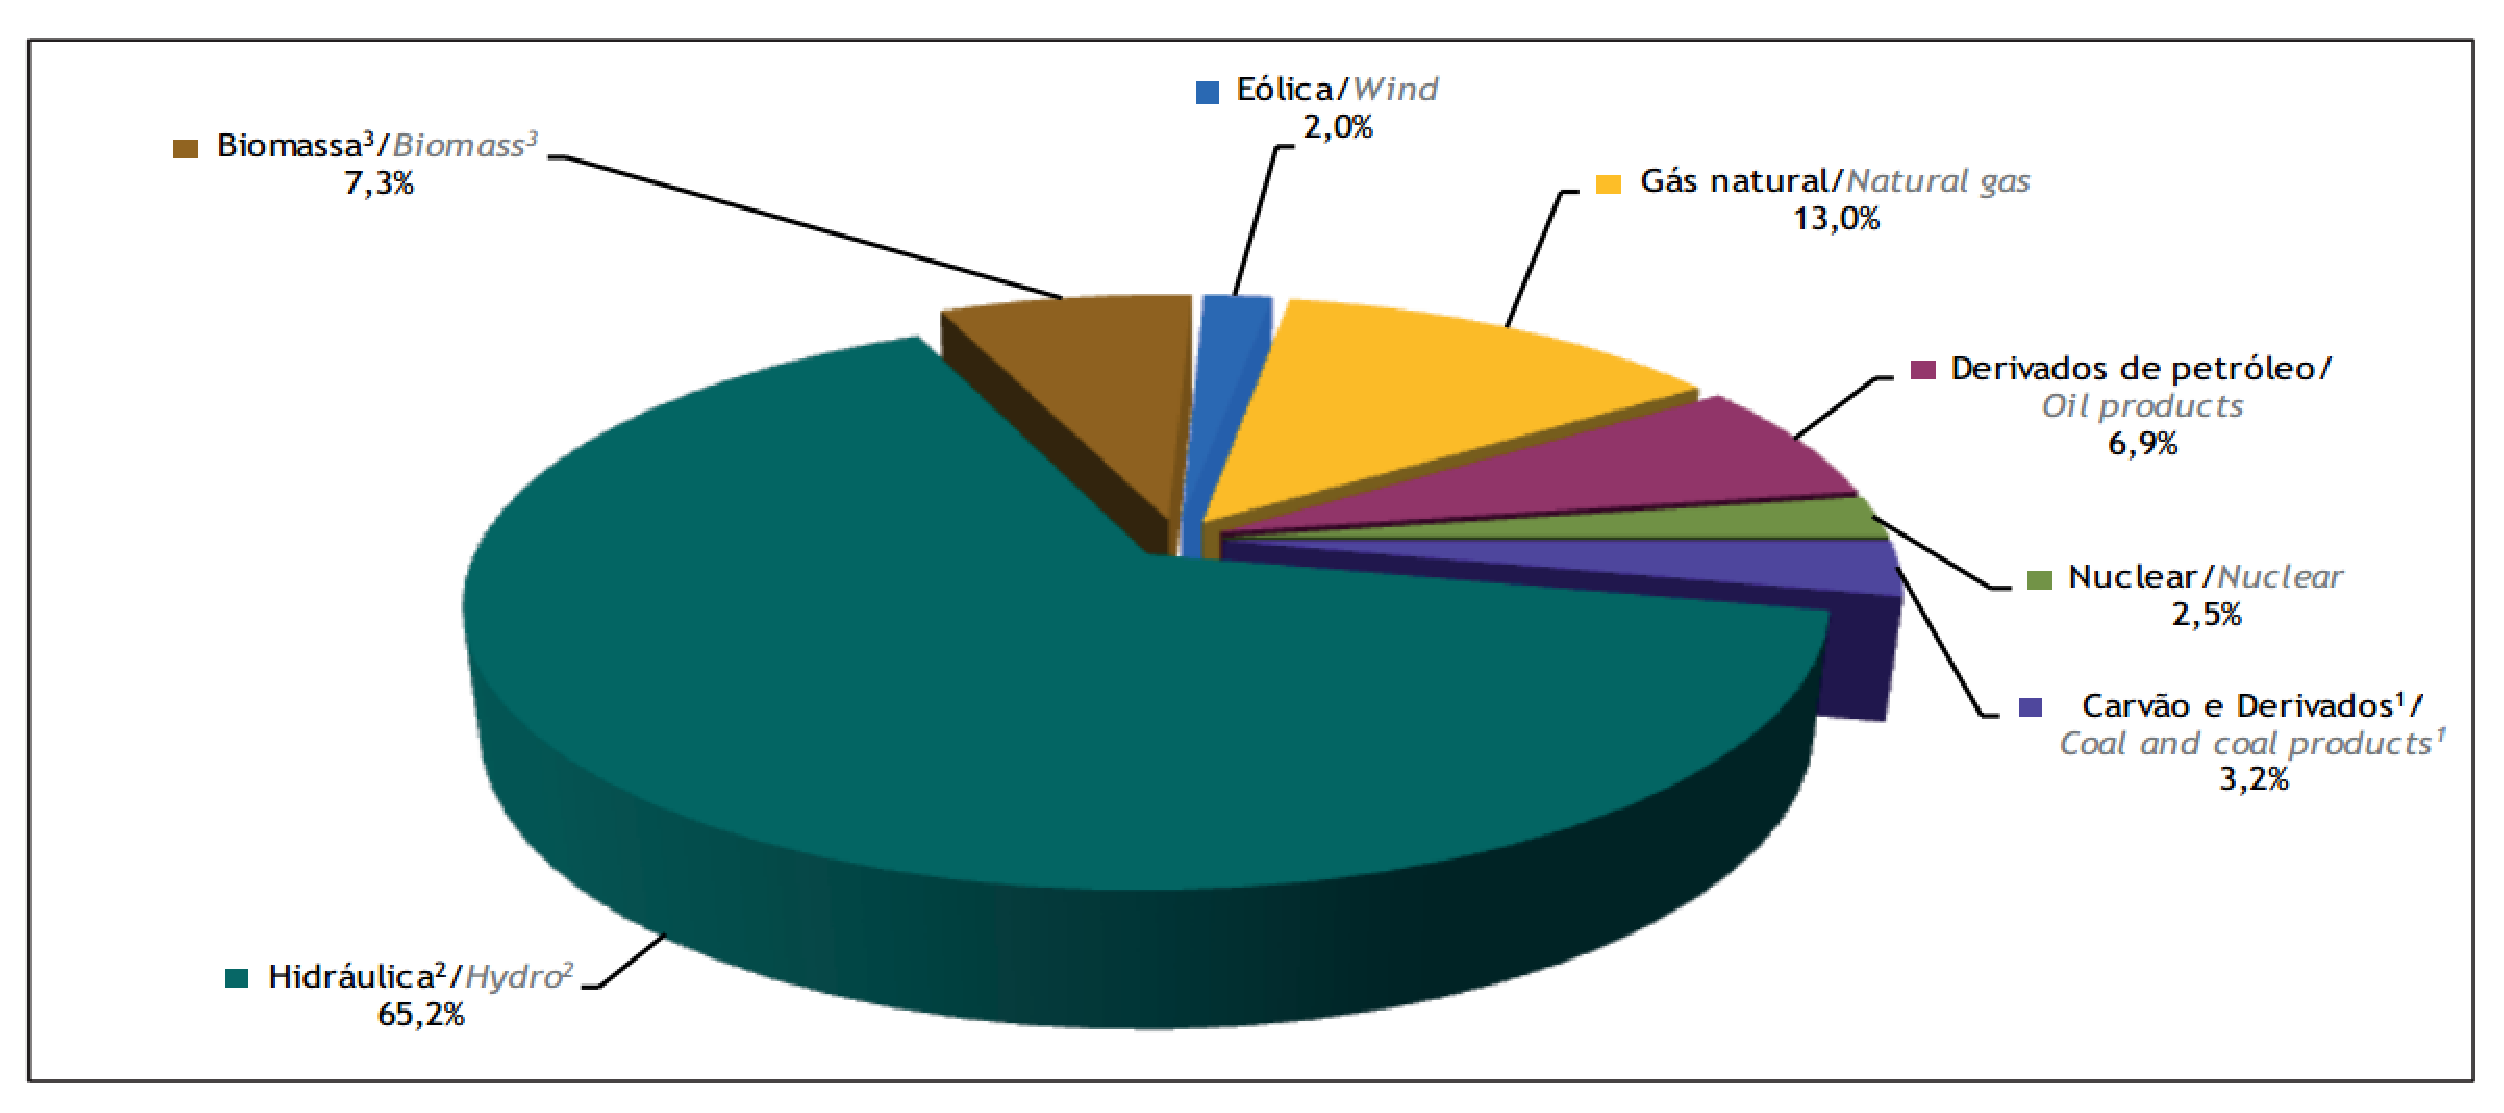
\includegraphics[keepaspectratio=true,scale=0.4]{figuras/consumo_energia_2014.eps}
    \caption{Oferta Interna de Eletricidade no Brasil em 2014}
    \label{consumo-2014}
\end{figure}

\section{Justificativa}
No ano de 2015 foi realizado um reajuste tarifário da energia elétrica correspondente à 33\% para clientes
residenciais e 32,5\% para empresas, indústrias e comércios \cite{aumento_energia}, ou seja, o uso abusivo dessa fonte
acarreta em gastos excessivos e desnecessários.

Dentre as alternativas para reduzir o consumo de energia elétrica encontram-se o uso de equipamentos mais eficientes, certificações Procel, uso racional da energia e afins, porém, quando se trata de instalações de grande porte, como Universidades e órgãos públicos em geral, percebe-se que um dos grandes problemas enfrentado é a falta de monitoramento adequado do uso de energia elétrica.

Idealiza-se que esse conhecimento de forma setorial do quanto está sendo consumido acarretará em uma analise preditiva e corretiva das instalações, visando uma maior conscientização dos usuários, consumo eficiente e economia.

A presente proposta destre trabalho encontra-se direcionada para o desenvolvimento, tendo como base os conhecimentos
adquiridos por um Engenheiro de Software, de um sistema de gerenciamento energético para uma instalação de grande porte referente à Universidade de Brasília.

\section{Objetivo Geral}
Desenvolver sistema web capaz de monitorar, em tempo real, medições de energia coletadas por transdutores
instalados em quadros de energia da Universidade de Brasília.

\subsection{Objetivos Específicos}
O sistema deve ser capaz de:
\begin{itemize}
    \item Cadastrar/Editar/Remover transdutores.
    \item Utilizar rede da universidade para comunicar-se com transdutores.
    \item Realizar a coleta de dados de forma automatizada e temporizada.
    \item Mostrar aos usuários os dados de energia coletados.
\end{itemize}

\section{Metodologia Utilizada}

\section{Estruturação do Trabalho}

\chapter{Metodologia}

\section{Métodos Ágeis}
Os negócios atualmente operam em um ambiente global sujeito a rápidas mudanças sendo crucial
estar preparado para novas oportunidades de mercado, mudanças de condições econômicas e ao surgimento
de produtos e serviços concorrentes. O \textit{software} é um dos componentes cruciais para a realização
de todas as operações de negócio e realizá-lo de forma rápida também é uma maneira de aproveitar novas
oportunidades e responder às pressões competitivas. \cite{sommerville_2006}

O manifesto ágil, \cite{beck2001agile}, consiste na base que fundamenta o desenvolvimento ágil de
\textit{software}, onde o mesmo é composto de quatro valores fundamentais:

\begin{itemize}
    \item Os indivíduos e suas interações acima de procedimentos e ferramentas;
    \item O funcionamento do software acima de documentação abrangente;
    \item A colaboração dos clientes acima da negociação de contratos;
    \item A capacidade de resposta a mudanças acima de um plano pré-estabelecido;
\end{itemize}

Além desses valores são definidos 12 princípios de agilidade:

\begin{itemize}
    \item Nossa maior prioridade é satisfazer o cliente, através da entrega adiantada e contínua de software de valor.
    \item Aceitar mudanças de requisitos, mesmo no fim do desenvolvimento. Processos ágeis se adequam a mudanças, para que o cliente possa tirar vantagens competitivas.
    \item Entregar software funcionando com freqüencia, na escala de semanas até meses, com preferência aos períodos mais curtos.
    \item Pessoas relacionadas à negócios e desenvolvedores devem trabalhar em conjunto e diariamente, durante todo o curso do projeto.
    \item Construir projetos ao redor de indivíduos motivados. Dando a eles o ambiente e suporte necessário, e confiar que farão seu trabalho.
    \item O Método mais eficiente e eficaz de transmitir informações para, e por dentro de um time de desenvolvimento, é através de uma conversa cara a cara.
    \item Software funcional é a medida primária de progresso.
    \item Processos ágeis promovem um ambiente sustentável. Os patrocinadores, desenvolvedores e usuários, devem ser capazes de manter indefinidamente, passos constantes.
    \item Contínua atenção à excelência técnica e bom design, aumenta a agilidade.
    \item Simplicidade: a arte de maximizar a quantidade de trabalho que não precisou ser feito.
    \item As melhores arquiteturas, requisitos e designs emergem de times auto-organizáveis.
    \item Em intervalos regulares, o time reflete em como ficar mais efetivo, então, se ajustam e otimizam seu comportamento de acordo.
\end{itemize}

Nem todos os processos ágeis aplicam tais princípios de maneira igualitária e alguns modelos escolhem ignorar (ou ao menos minimar) a importância de um ou mais princípios. \cite{pressman_2009}

Segundo \cite{sommerville_2006}, processos de desenvolvimento ágeis geralmente são iterativos onde a
especificação, projeto, desenvolvimento e teste são intercalados. O \textit{software} é desenvolvido
em uma série de incrementos e cada incremento fornece uma nova funcionalidade ao sistema. As duas principais
vantagens de se adotar uma abordagem incremental para o desenvolvimento de \textit{software} são:

\begin{itemize}
    \item Entrega acelerada dos serviços ao cliente. Os clientes poderão obter valor do sistema com incrementos iniciais.
    \item Engajamento do usuário com o sistema. Os usuários do sistema devem estar envolvidos no processo
    de desenvolvimento dando \textit{feedback} à equipe de desenvolvimento sobre os incrementos entregues.
\end{itemize}

\section{\textit{Extreme Programming}}
Segundo \cite{beck_2004}, \textit{Extreme Programming} (XP) é uma filosofia de desenvolvimento de
\textit{software} baseada nos valores de comunicação, \textit{feedback}, simplicidade, coragem e respeito.
Por ser um tipo de metodologia ágil de desenvolvimento de \textit{sofwtare} são defendidas \textit{releases}
frequentes, as quais devem possuir curtos ciclos de desenvolvimento, destinadas à aumentar a produtividade, qualidade de \textit{software} e introduzir pontos de controle para que novas necessidades dos clientes sejam atendidas.

Práticas do XP:

\begin{itemize}
    \item Testar cedo, com frequência e automação.
    \item \textit{Design} incremental.
    \item Implantação diária.
    \item Envolvimento do cliente.
    \item Integração contínua.
    \item Ciclos de desenvolvimento curtos.
    \item Planejamento incremental.
    \item Programação em pares.
\end{itemize}

\section{Scrum}
Scrum.
O que é sprint.
Reunião de planejamento de sprint com orientador e cliente.

\section{Sofware Livre}

\section{Licença de Software}
MIT

\section{Cronograma}

\chapter{Ciclo de Vida do Sistema}
\section{Definição da Abordagem e Metodologia}
Como a parte inicial do projeto, com um período de aproximadamente 6 meses, seria realizada pelo próprio autor, a disponibilidade do cliente ser mais abrangente, o projeto for evoluido conforme o tempo e novas necessidades forem surgindo, definiu-se a utilização de uma abordagem de desenvolvimento ágil \cite{beck2001agile}.


A metodologia utilizada baseou-se no Kanban \cite{radigan_2015} com algumas práticas do \textit{Extreme Programming}.

A metodologia definida foi o  \cite{beck_2004}, visando sempre estar evoluindo o sistema com \textit{feedbacks} do cliente, produzindo código com padrões de codificação e simples para possíveis manuntenções no futuro.



Matheus Faria. Canbam. Produto nao finalizado, crescendo aos poucos, Sutherland. ciclo de desenvolvimento sem ter fim, pois projeto é grande.

Para auxiliar nas \textit{releases} do projeto, utilizou-se o conceito de \textit{sprints}, provinda do \textit{Scrum} \cite{scrum_guide}. As \textit{sprints} são pequenos intervalos de tempo, de um mês ou menos, durante o qual uma versão incremental potencialmente utilizável do produto é criada. Uma nova Sprint inicia imediatamente após a conclusão da Sprint anterior.

\section{Contexto e Necessidades}
Tendo como problema a falta de monitoramento energético adequado na Universidade de Brasília, foi realizado um estudo sobre o contexto para identificar as necessidades do cliente. Tal estudo abordava o entendimento de fatores energéticos cruciais, como por exemplo sistemas trifásicos, horários de ponta e fora de ponta, tensão, corrente, resistência e afins.

Explicar as grandezas, energia custa dinheiro, etc. redirecionar um gasto em ponta para fora de ponta.

Com um entendimento melhor do contexto, algumas reuniões foram feitas com o cliente e foram obtidas as seguintes necessidades:

\begin{itemize}
    \item Cada campus da Universidade de Brasília deve ser responsável por realizar seu próprio monitoramento energético.
    \item O campus Darcy Ribeiro deve funcionar como uma espécie de administração central.
    \item As medições devem ser registradas e poderão ser resgatadas, conforme um período de tempo especificado.
\end{itemize}

Cliente loana e alex representando unb, como cliente.

Buscando atender toda a conectividade esperada pelo projeto e trazer benefícios ao cliente, definiu-se que sistema teria uma implementação \textit{web}. Sistemas \textit{web} não necessitam de instalação por parte do usuário final, facilitando bastante o processo de implantação e podem ser acessados a partir de qualquer lugar e em qualquer plataforma \cite{pressman_2009}.

Um dos pontos levantados nas reuniões foi o de um possível monitoramento, no futuro, de medições de água. Tendo em vista esses recursos que seriam monitorados e de possíveis outros, definiu-se o nome do projeto como Sistema de Monitoramento de Insumos - Universidade de Brasília (SMI-UnB). Definiu-se, também, que para o contexto inicial seriam enfatizados os dados de energia e que seriam entregues duas \textit{releases}, de aproximadamente 80 dias, sendo essas:

\begin{itemize}
    \item Release 1: coleta dos dados de energia.
    \item Release 2: apresentação dos dados e prorótipo de comunicação inter-campi.
\end{itemize}

Deginiu-se que a hospedagem do código/documentação do projeto e o controle de mudanças seriam realizados utilizando-se o software livre GitLab CE\footnote{\url{https://gitlab.com/gitlab-org/gitlab-ce}} e para controlamento de versão, a ferramenta Git\footnote{\url{https://git-scm.com/}}.

A escolha do GitLab CE se deve pela cultura de software livre, pois o projeto teria um âmbito acadêmico, o compartilhamento de conhecimento poderia ser realizado de maneira mais fácil e a qualidade final não seria comprometida \cite{raymond1999}.

A licença escolhida para o projeto foi a MIT. Ela consiste em uma licença permissiva, autorizando o uso comercial, modificação, distribuição e sublicenciamento \cite{mit_license}

Grande uso meio academico, desenvolvida por uma universidade importante. A unb nao tem um modelo de refêrencia para software livre. o sublicenciamento seria necessário para a unb poder mudar a licença depois.

\section{Requisitos}
Com as necessidades em mãos e o repositório do projeto criado, utilizou-se o propósito das estórias de usuário \cite{beck_2004}, de uma maneira mais simplificada, em \textit{milestones} no repositório, as quais possuiriam diversas \textit{issues} e essas \textit{issues} apresentariam uma terminologia mais técnica da solução em si. Uma \textit{milestone} pode possuir uma data início/fim e é composta por um aglomerado de problemas, comumente chamados de \textit{issues} \cite{gitlab}.

Vale ressaltar que as \textit{milestones} e \textit{issues} foram criadas acompanhando o decorrer do projeto, ou seja, a cada \textit{sprint}, era avaliado se ocorreram mudanças de escopo, quais seriam as \textit{issues} da próxima \textit{sprint}, se era necessário criar uma nova \textit{milestone} etc.

\section{Implantação - Devops}
Contínuo, desenvolvimento com implantação.

Filosofia, nível de automatização alto.

Tasks

Containers utilizados.

\section{Desenvolvimento}
Será explicado depois
\chapter{Características do SMI-UnB}

\section{Tecnologias Escolhidas}


Definiu-se utilizar o \textit{framework} \textit{web} Django, por o mesmo realizar facilmente a integralização, desde a comunicação com o banco de dados até a apresentação de dados para o usuário final. Além disso, o banco de dados escolhido foi PostgreSQL, que assim como o Django, também trata-se de um software livre.

    \subsection{Django}

    O Django \cite{django_project} é um \textit{framework} para desenvolvimento \textit{web} implementado na linguagem Python\footnote{\url{https://www.python.org/}}. Sua arquitetura inspira-se no modelo tradicional MVC(\textit{Model} \textit{View} \textit{Controller}), porém, com algumas especificidades. A comunidade \textit{Django} adota o acrônimo MTV (\textit{Model} \textit{Template} \textit{View}), onde os papéis de \textit{model}, \textit{view} e \textit{controller} são redefinidos como:
    \begin{itemize}
        \item \textit{Model}: corresponde à \textit{model} do MVC tradicional e representa as classes que popularão as tabelas do banco de dados. O \textit{Django} possui um ORM (\textit{Object-Relational Mapping}, Mapeamento de Objeto Relacional) para realizar a manipulação dessas tabelas, não sendo necessário a escrita de consultas em SQL para a persistência das informações.
        \item \textit{Template}: corresponde aproximadamente à \textit{view} do MVC tradicional e descreve como as informações serão apresentadas para o usuário.
        \item \textit{View}: representada por uma função \textit{callback} referente à uma classe de URLs, descrevendo quais informações serão apresentadas e como elas serão enviadas para o \textit{template}. Alguns autores defendem que a view corresponde ao \textit{controller} do MVC tradicional, mas os próprios desenvolvedores do \textit{Django} a \textit{view} deve ser minimalista e boa parte do papel do \textit{controller} deve ser implementado nas próprias classes dos modelos.
    \end{itemize}

    Na nomenclatura do \textit{Django}, um conjunto de funcionalidades pode ser agrupado em aplicação. Cada aplicação possui suas próprias \textit{models}, \textit{views} e \textit{templates}.

    A Figura \ref{django-arq} mostra a arquitetura do \textit{Django}, apresentando as camadas do MTV durante a comunicação com o navegador até o acesso ao banco de dados. O \textit{URL dispatcher} identifica endereços requisitados pelo usuário e realiza o redirecionamento da requisição para a aplicação correta. A coordenação de requisições entre o \textit{URL dispatcher} e a \textit{view} e da \textit{view} até o \textit{template} é feita pelos chamados \textit{Middlewares}. Os \textit{Middlewares} realizam a persistência de informações entre as diferentes camadas.

    \begin{figure}[h]
        \centering
        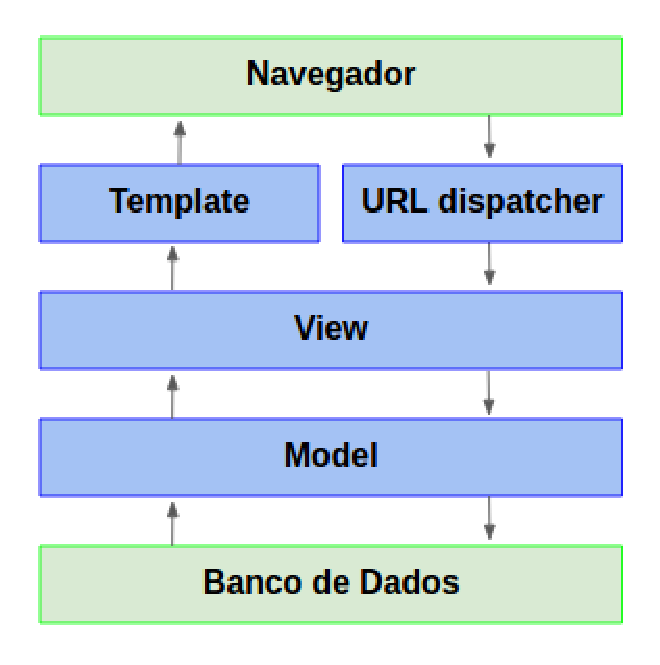
\includegraphics[keepaspectratio=true,scale=0.5]{figuras/django-arquitetura.eps}
        \caption{Arquitetura MTV \textit{Django}}
        \label{django-arq}
    \end{figure}

\section{Protocolos Utilizados}
Antes de começar o desenvolvimento, foi necessário realizar um profundo estudo sobre o equipamento para medição de dados de energia, comumente chamado de transdutor, visto que esse já havia sido pré-designado para utilização, devido a contratos realizados anteriormente pela Universidade de Brasília.

O equipamento em questão foi o TR 4020, Figura \ref{tr4020}, disponibilizado pela empresa Embrasul\footnote{\url{http://www.embrasul.com.br/}}. Segundo seu manual, possui frequência de amostragem a cada 50ms, comunica-se utilizando o protocolo de comunicação Modbus, no modo RTU com velocidade de 10M/100Mbps em sistemas Ethernet utilizando o protocolo UDP como transporte. No datagrama UDP, no campo de dados, o protocolo ModBUs - RTU é encapsulado, sendo que a porta de comunicação padrão é a 1001. O endereço ModBus dos equipamentos por padrão é 1, onde a diferenciação entre equipamentos se dá pelo número de IP.

\begin{figure}[h]
    \centering
    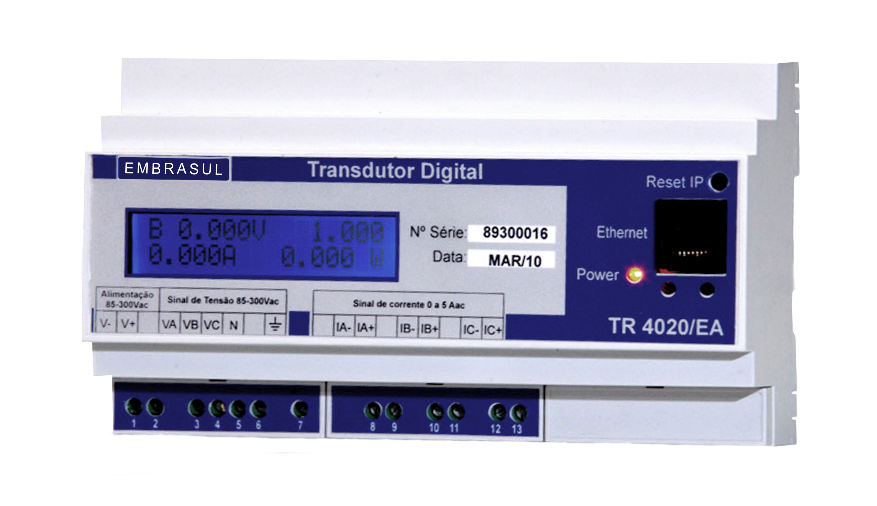
\includegraphics[keepaspectratio=true,scale=0.5]{figuras/tr4020.eps}
    \caption{Transdutor TR4020}
    \label{tr4020}
\end{figure}

    \subsection{\textit{Modbus RTU}}

    \textit{Modbus} é um protocolo serial utilizado para transmitir informações entre dispositivos eletrônicos. Suas mensagens utilizam a arquitetura de mestre-escravo, como mostrado na figura \ref{mestre_escravo} \cite{modbus}. Nesta arquitetura, o papél de mestre é designado ao dispositivo que envia as requisições e escravo ao que responde passivamente às mesmas.

    \begin{figure}[!htpb]
        \centering
        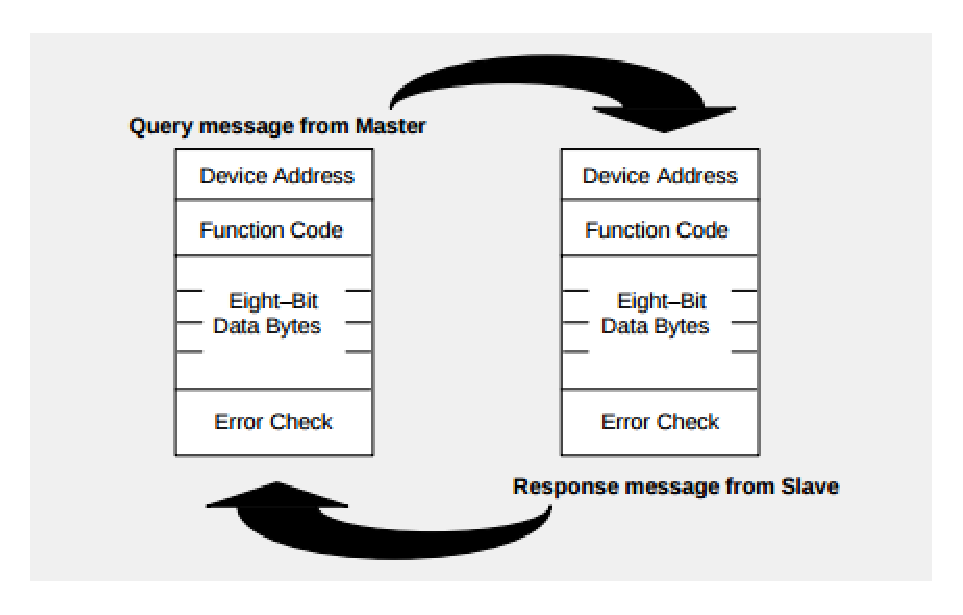
\includegraphics[keepaspectratio=true,scale=0.8]{figuras/mestre_escravo.eps}
        \caption{Comunicação Mestre-Escravo \textit{Modbus}. Fonte: \cite{modbus}}
        \label{mestre_escravo}
    \end{figure}

    Quando controladores são configurados para se comunicarem em uma rede Modbus usando o modo RTU (\textit{Remote Terminal Unit}, Unidade de Terminal Remoto) cada \textit{byte} contém duplas hexadecimais de 4 \textit{bits}. A maior vantagem de utilizar este modo é que sua grande densidade de caracteres permite uma maior taxa de transferência comparado ao modo ASCII em uma mesma taxa de transmissão \cite{modbus}.

    Uma mensagem em Modbus RTU possui 16 \textit{bytes} e é definida da seguinte maneira:
    \begin{itemize}
        \item Identificador do Aparelho: 2 \textit{bytes}.
        \item Código de Função: 2 \textit{bytes}, define qual tipo de operação o equipamento irá realizar.
        \item Campo de Dados: 8 \textit{bytes}, sendo 4 \textit{bytes} para indicar o endereço do primeiro registrador requisitado e 4 \textit{bytes} para indicar a quantidade de registradores que serão lidos.
        \item CRC (\textit{Cyclic Redundancy Check}, Verificação de Redundância Cíclica): 4 \textit{bytes} para verificação de erros.
    \end{itemize}

    A resposta do escravo possui a seguinte estrutura:

    \begin{itemize}
        \item Identificador do Aparelho: 2 \textit{bytes}.
        \item Código de Função: 2 \textit{bytes}, define qual tipo de operação o equipamento irá realizar.
        \item Tamanho do{payload}: 2 \textit{bytes}, define o tamanho do campo de dados em \textit{bytes}.
        \item Campo de dados: possui tamanho variável, de acordo com o valor do campo anterior.
        \item CRC (\textit{Cyclic Redundancy Check}, Verificação de Redundância Cíclica): 4 \textit{bytes} para verificação de erros.
    \end{itemize}

    \subsection{UDP}
    A camada de transporte é...

    Ethernet é...

    IP é...

    O protocolo UDP (\textit{User Datagram Protocol}, Protocolo de Datagrama do Usuário) é um protocolo da camada de transporte e não orientado a conexões. Seu cabeçalho, figura \ref{udp_header}, possui 8 \textit{bytes}, seguido de uma carga útil. As portas apresentadas no cabeçalho representam as máquinas de origem e destino \cite{tanenbaum_2002}.

    \begin{figure}[!htpb]
        \centering
        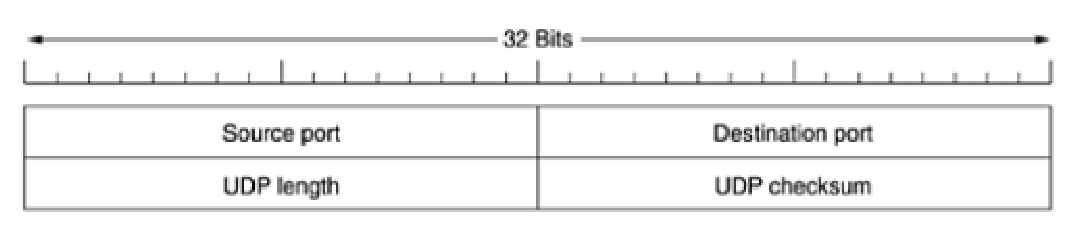
\includegraphics[keepaspectratio=true,scale=0.8]{figuras/udp_header.eps}
        \caption{Cabeçalho do UDP. Fonte: \cite{tanenbaum_2002}}
        \label{udp_header}
    \end{figure}

\section{Coleta e Sincronia de Dados}
Data reader

Cronjob

Protótipo API
\section{Segurança}
Autenticaçao por email

Senhas incriptadas no banco de dados (pelo django)

Secret key gerada automaticamente

Permissões do sistema

Nao pode excluir transdutores ou prédios
\section{Gerência de Configuração}
Runner do Gitlab-CI (Interação Contínua)

Tasks

Fixtures

Docker
    ambiente de produção
    Docker-compose (Nginx, gunicorn, postgresql, redis)
\section{Apresentação das Informações}
Bootstrap

Javascripts usados

Gráficos

Imagens da aplicação
\section{Métricas}
Codeclimate

sloccount

\section{Visão Geral do Sistema}
    \subsection{Diagrama de Classes}
    Interessante para quem quer entender o sistema (Software livre)

    Apresentar diagrama
    \subsection{Testes}
    Testes unitários com Mock

    Cobertura
    \section{Requisitos Mínimos}
    Rodar linux

    Rede?

\chapter{Conclusão}

\section{Trabalhos Futuros}
Tendo como base o que foi realizado neste trabalho, percebe-se que é possível aprimorar o sistema construído acrescentando algumas funcionalizades a mais:
\begin{itemize}
    \item Envio de dados em tempo real para a central
    \item 
\end{itemize}

\section{Cronograma}

% \chapter{Visão Geral do Sistema Desenvolvido}

O levantamento adequado de requisitos de software é crucial para
que possa ser feito um mapeamento das reais necessidades do cliente com
funcionalidades que um sistema deve atender. Sommerville \cite{sommerville_2006}
destingue bem essas abordagens como ``requisitos do usuário'' e ``requisitos do sistema''. Os requisitos de usuários consistem de declarações, em
linguagem natural, que o sistema deve fornecer e restrições que o mesmo deve
operar. Os requisitos de sistema estabelecem de maneira detalhada as
funções e restrições do sistema. Além disso, os requisitos de sistema
classificam-se em funcionais e não funcionais:

\begin{itemize}
    \item Requisitos Funcionais: declaração de funções que o sistema deve fornecer, como o mesmo irá reagir com certas entradas e como deve se comportar para certas situaçoes.
    \item Requisitos Não Funcionais: restrições sobre serviços ou funções oferecidas pelo sistema.
\end{itemize}

Objetivando levantar os requisitos do sistema, realizaram-se reuniões com o
cliente e os requisitos obtidos foram os seguintes:

\begin{itemize}
    \item Funcionais:
    \begin{itemize}
        \item O sistema deve ser capaz de realizar um monitoramento temporal de recursos energéticos.
        \item O sistema deve ser capaz de gerar gráficos com as medições de energia obtidas.
        \item O sistema deve permitir a autenticação de usuários com diferentes níveis de acesso.
        \item O sistema deve permitir o gerenciamento de usuários, prédios e aparelhos de medição.
        \item O sistema deve permitir que usuários atualizem suas informações básicas.
    \end{itemize}
    \item Não Funcionais:
    \begin{itemize}
        \item O
    \end{itemize}
\end{itemize}

Com os requisitos obtidos, realizou-se uma atribuição dos mesmos para
as iterações do projeto, onde cada iteração possuiria um ou mais requisitos,
que eram mapedos, de maneira mais simplificada, em uma \textit{milestone} no repositório oficial do projeto.
As \textit{milestone} representariam um requisito e possuiriam um conjunto
de tarefas (\textit{issues}), que após serem finalizadas, concluiriam
o requisito representado pela mesma.
% \chapter{Gerenciamento de Configuração}

\section{Controle de Versão}

\section{Política de Branchs}

\section{Integração Contínua}

% \chapter{Evolução do Sistema}

\section{Sprint 01 (25/07/2016 à 05/08/2016) - Coleta Inicial de Dados Transdutor}
Buscando realizar uma primeira análise do transdutor instalado na Universidade, verificando se a comunicação com o mesmo poderia ser realizada de maneira efetiva, realizou-se o módulo \textit{data\_reader} contendo as seguintes classes:
\begin{itemize}
    \item Transductor: representação de um transdutor.
    \item Measurements: representação das medições de energia realizadas pelo transdutor.
    \item CommunicationProtocol: acoplamento dos protocolos de transporte e serial, visando realizar uma comunicação com o transdutor.
\end{itemize}

A figura \ref{sprint01arq} representa a arquitetura inicial do projeto, onde basicamente um transdutor possui várias medições de energia e, dependendo do seu modelo, pode possuir diferentes protocolos para se comunicar.

\begin{figure}[!htpb]
    \centering
    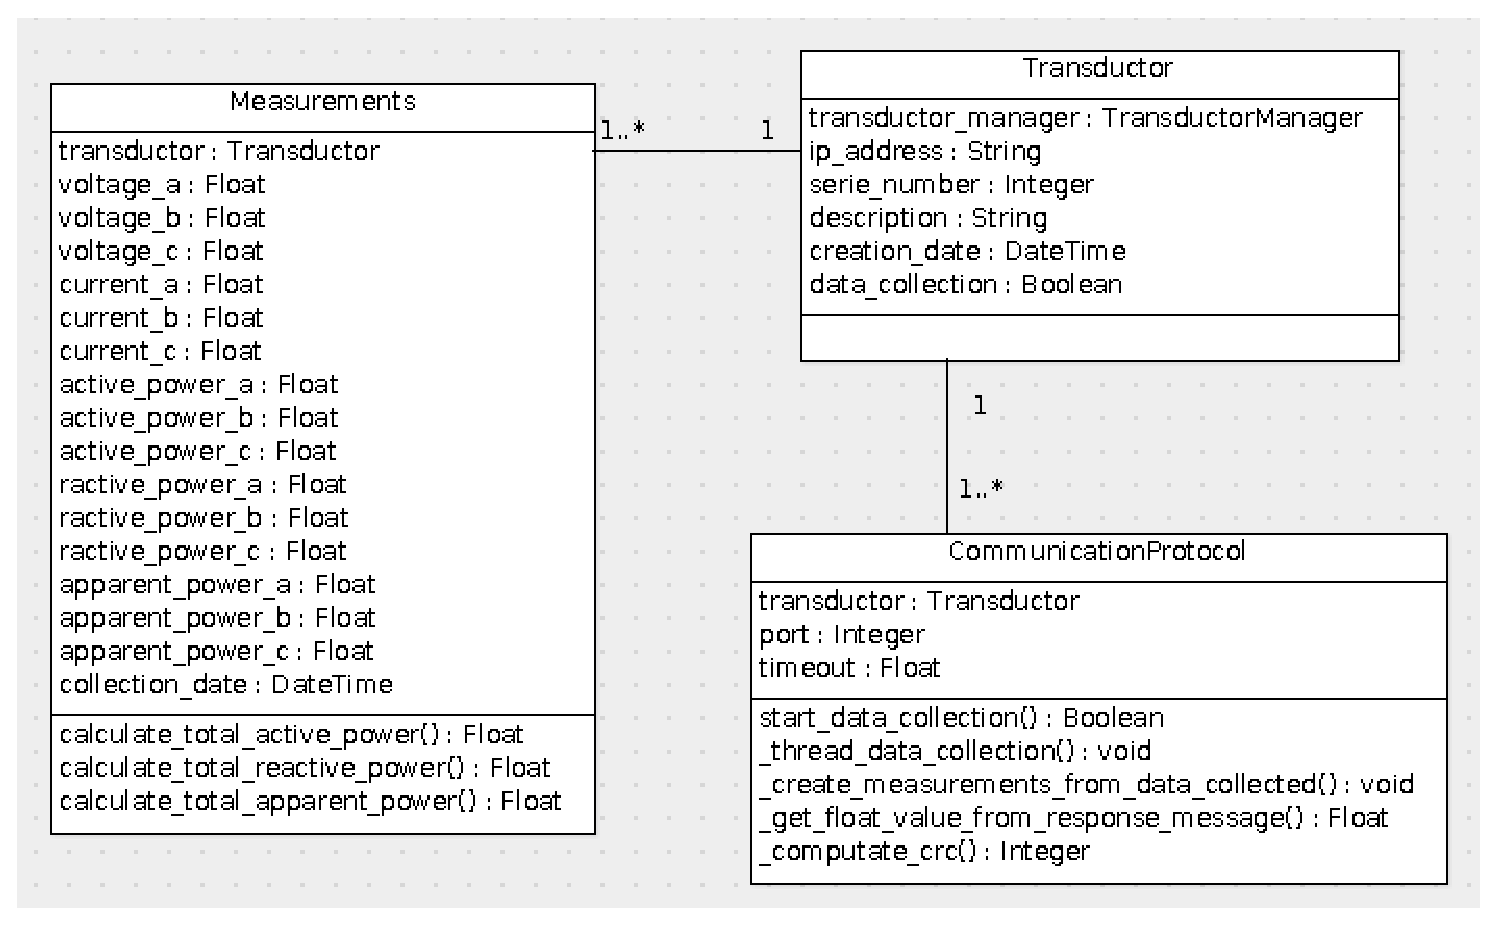
\includegraphics[keepaspectratio=true,scale=0.6]{figuras/sprint01arq.eps}
    \caption{Arquitetura SME-UnB \textit{Sprint 01}. Fonte: autor}
    \label{sprint01arq}
\end{figure}

\vfill
\pagebreak

Foram realizar algumas telas, figuras \ref{dados01} e \ref{dados02}, contendo os dados de energia coletados para apresentação ao usuário.

\begin{figure}[!htpb]
    \centering
    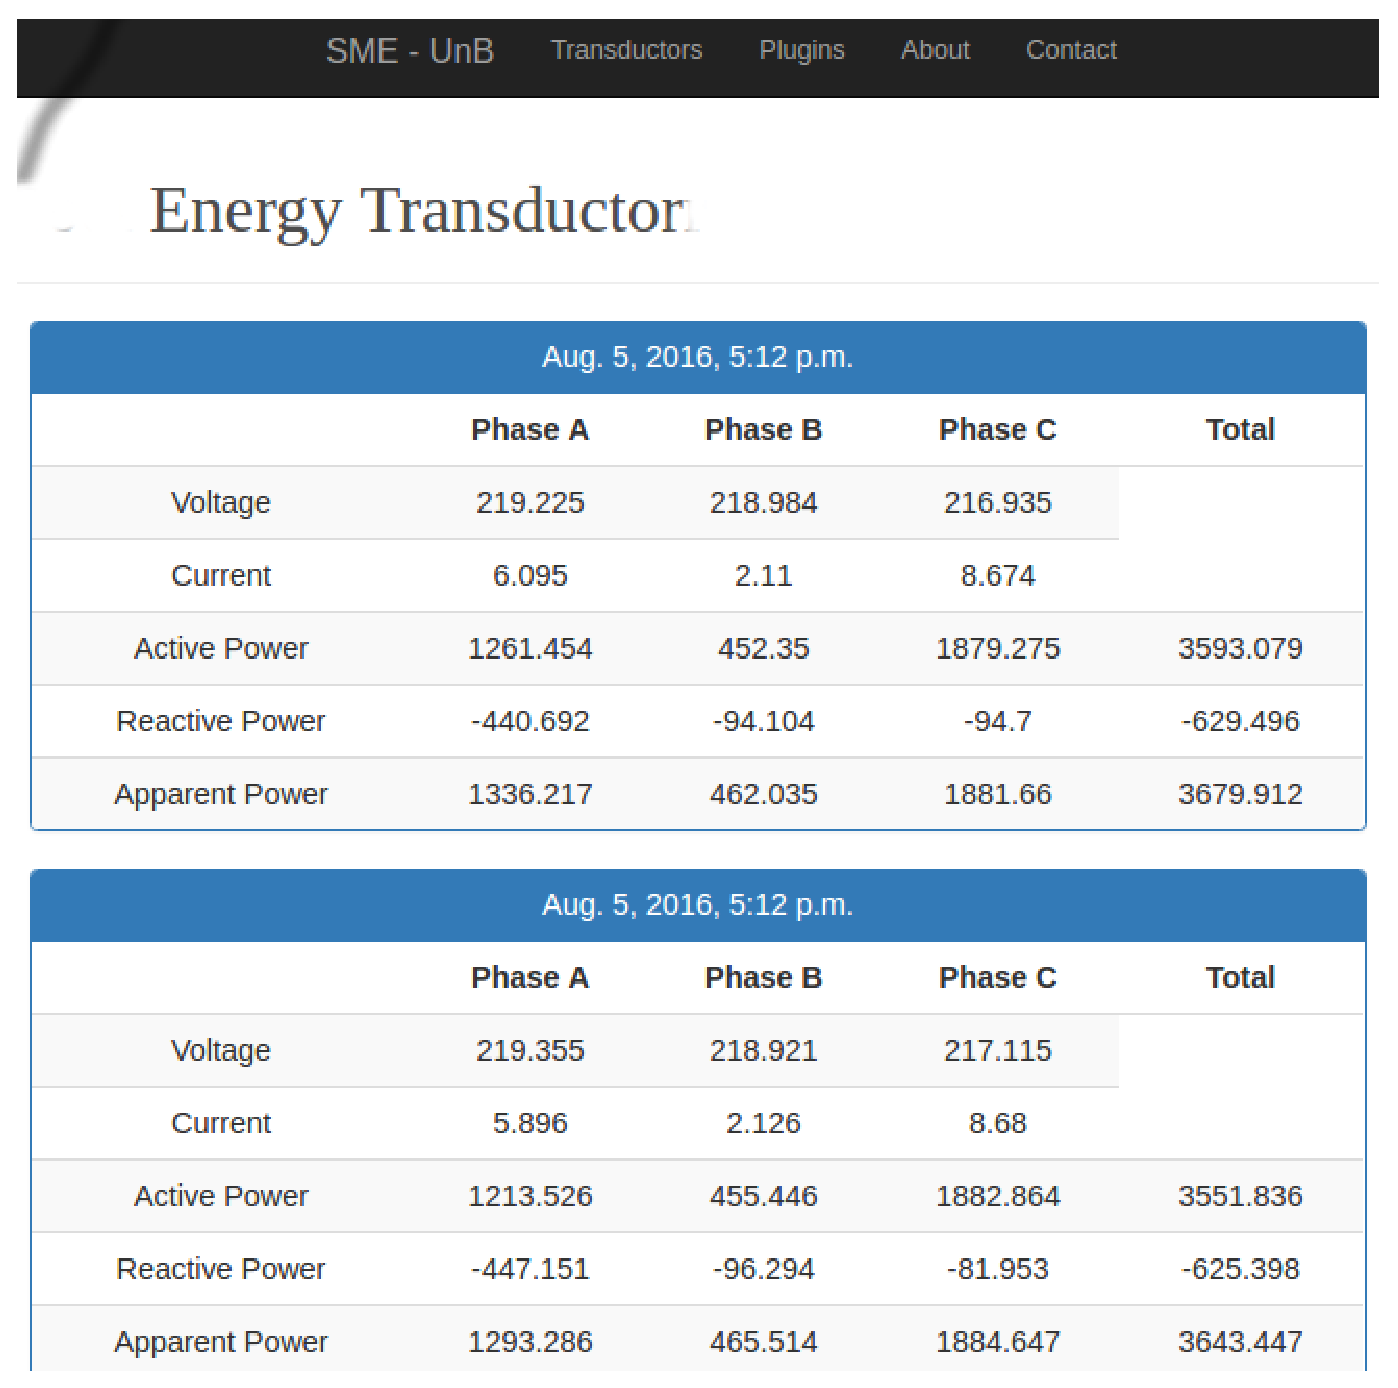
\includegraphics[keepaspectratio=true,scale=0.5]{figuras/coleta_dados_01.eps}
    \caption{Página apresentação medições de energia. Fonte: autor}
    \label{dados01}
\end{figure}

\begin{figure}[!htpb]
    \centering
    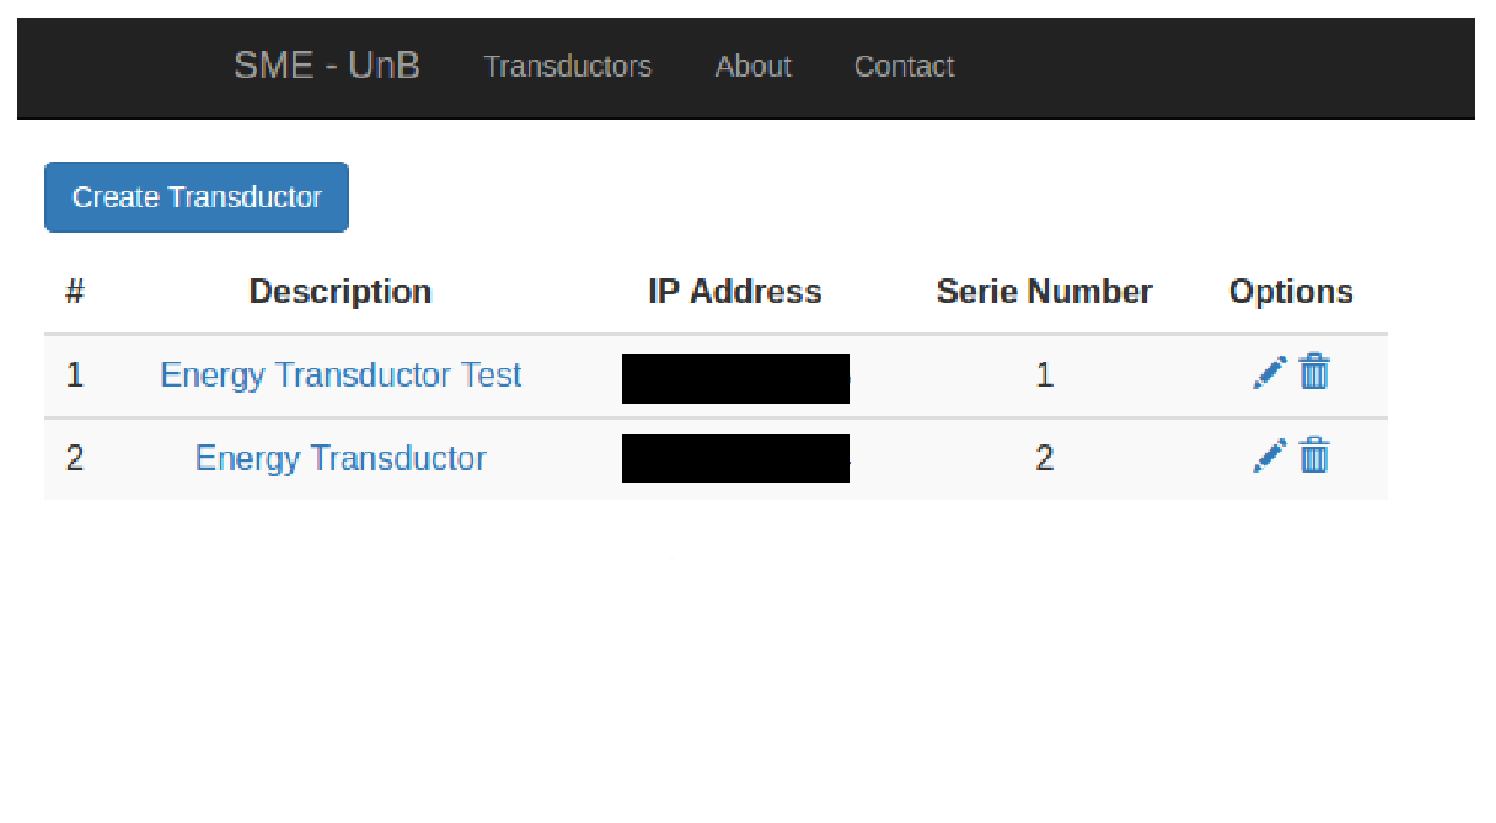
\includegraphics[keepaspectratio=true,scale=0.5]{figuras/coleta_dados_02.eps}
    \caption{Página apresentação medições de energia. Fonte: autor}
    \label{dados02}
\end{figure}

\vfill
\pagebreak

\section{Sprint 02 (08/08/2016 à 19/08/2016) - Refatorações de Urls/Templates e Guia de Instalação}
Após analisadas as urls e templates do projeto verificou-se que haviam muitas rotas desnecessárias e não havia um padrão para os templates, o que estava gerando confusão na hora de criar novas páginas para a aplicação. Tendo em mente tais problemas essa sprint buscou realizar uma refatoração dos mesmos.

Realizou-se um guia de instalação\footnote{\url{https://gitlab.com/brenddongontijo/SME-UnB/wikis/instalation-guide/}} para o ambiente de desenvolvimento utilizando as ferramentas Vagrant\footnote{\url{https://www.vagrantup.com/}} e Chef Solo\footnote{\url{https://docs.chef.io/chef_solo.html}}, visando auxiliar novos desenvolvedores a contribuirem com o projeto.

\section{Sprint 03 (22/08/2016 à 02/09/2016) - Reestruturação Arquitetura e Primeiros Testes}
Realizou-se uma reunião com o orientador visando reestruturar a arquitetura. Primordialmente, tendo em vista que os tradutores podem possuir diferentes tipos de medições, foram definidas duas classes abstratas: Transductor e Measurements. A partir dessas classes surgiram as especializações de transdutores de energia (EnergyTransductor) e medições de energia (EnergyMeasurements). Além disso, percebeu-se a necessidade de criação de um modelo de transdutor (TransductorModel), o qual possuiria informações específicas do mesmo, como endereço e tipo dos registradores, protocolo serial e de transporte utilizados. A figura \ref{sprint03arq} ilustra a evolução da arquitetura realizada nessa sprint.

\begin{figure}[!htpb]
    \centering
    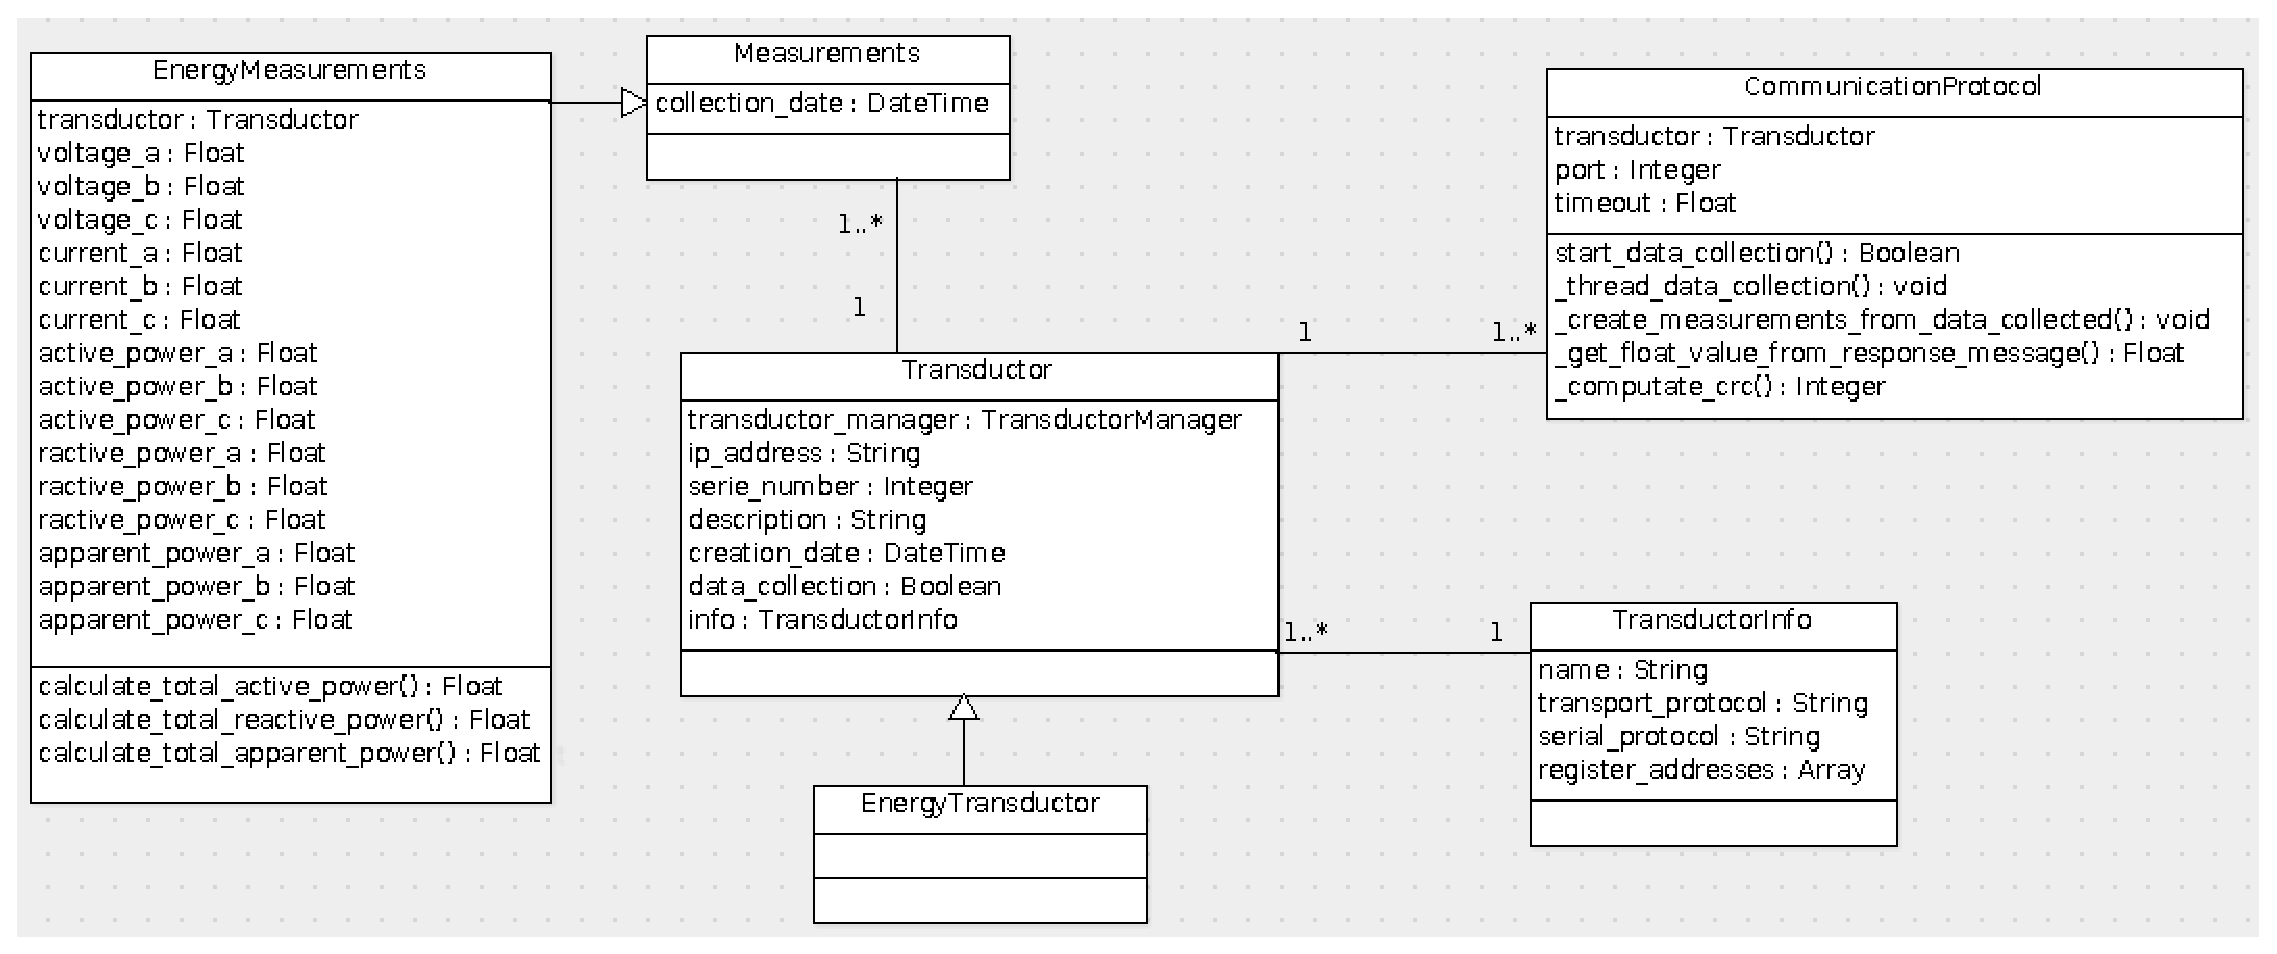
\includegraphics[scale=0.6,angle=90]{figuras/sprint03arq.eps}
    \caption{Arquitetura SME-UnB Sprint 03. Fonte: autor}
    \label{sprint03arq}
\end{figure}

\vfill
\pagebreak

Nessa sprint foi realizado um primeiro contato com os testes e ao seu fim foi obtivo uma cobertura total de 71\%, conforme a figura \ref{cobertura01}.

\begin{figure}[!htpb]
    \centering
    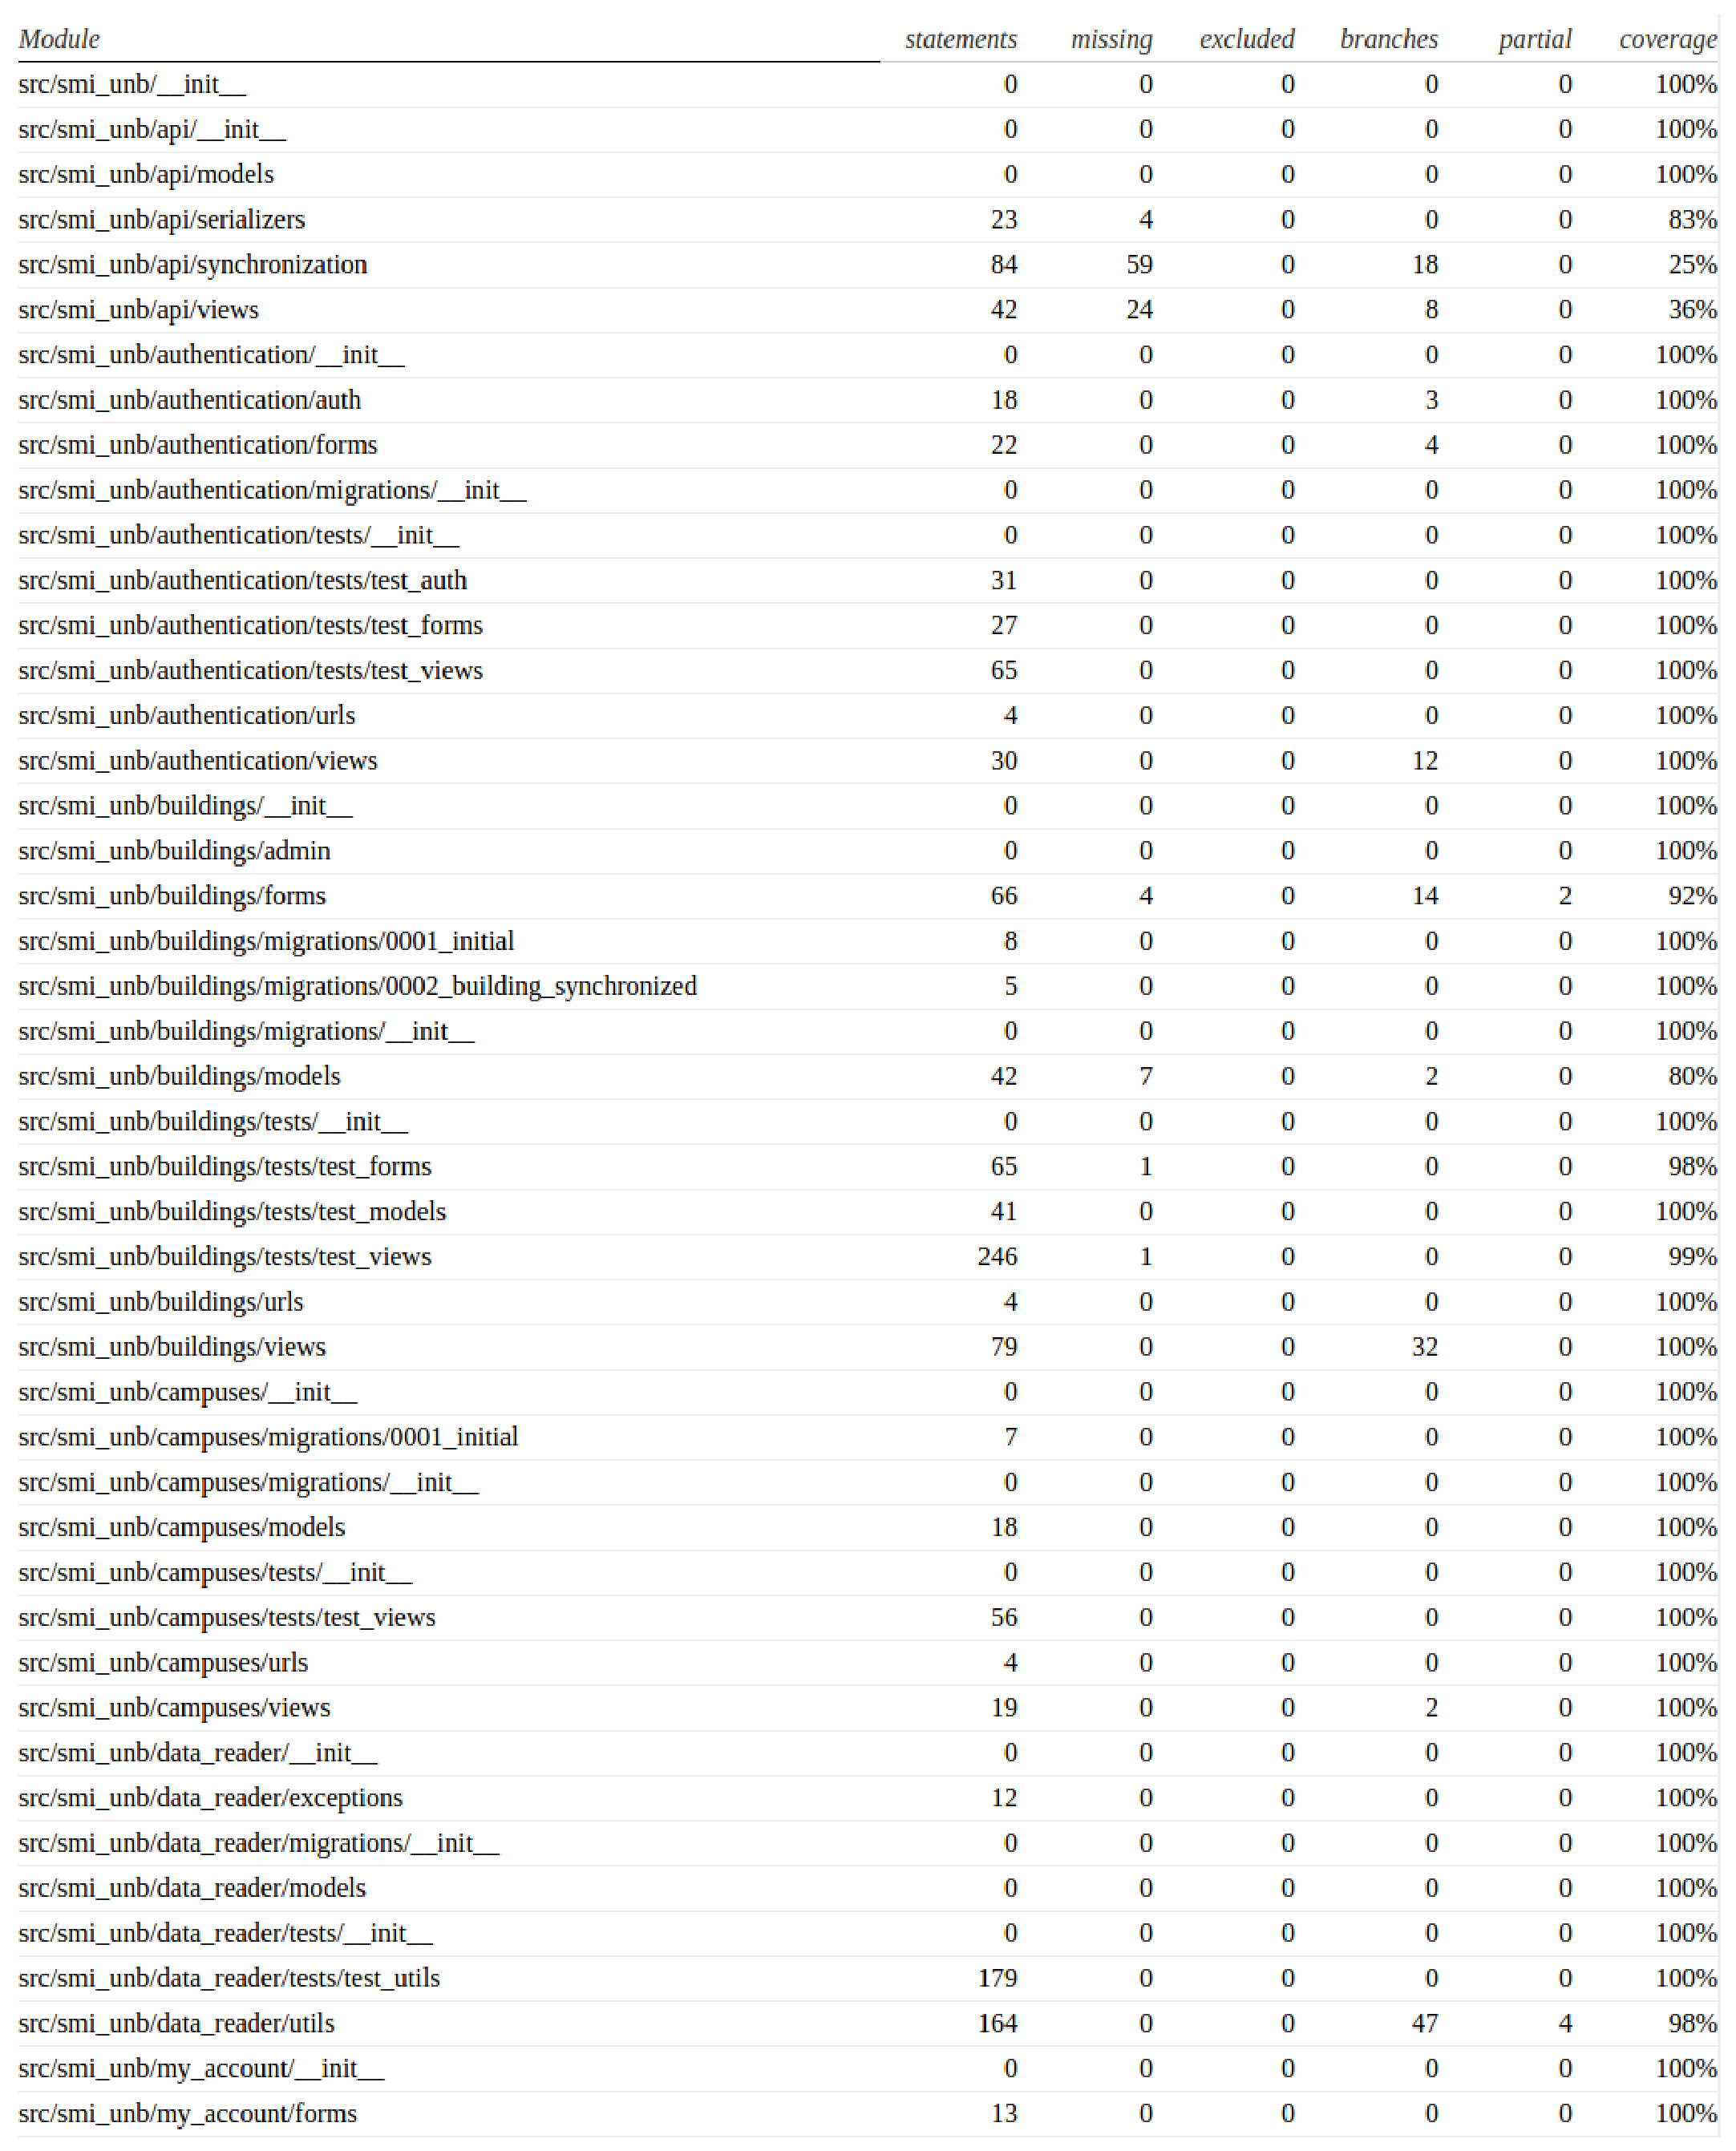
\includegraphics[keepaspectratio=true,scale=0.5]{figuras/cobertura01.eps}
    \caption{Cobertura Total de Código Sprint 03. Fonte: autor}
    \label{cobertura01}
\end{figure}

\section{Sprint 04 (05/09/2016 à 16/09/2016) - Documentação de Código e Estrutura \textit{Boilerplate}}
Buscando deixar o código mais entendível realizou-se uma documentação geral utilizando os padrões de \textit{docstrings}\footnote{\url{https://www.python.org/dev/peps/pep-0257/}} definidos pelo \textit{Google Python Style}\footnote{\url{http://google.github.io/styleguide/pyguide.html}}. A figura \ref{documentacao01} ilustra um exemplo realizado no projeto.

\begin{figure}[!htpb]
    \centering
    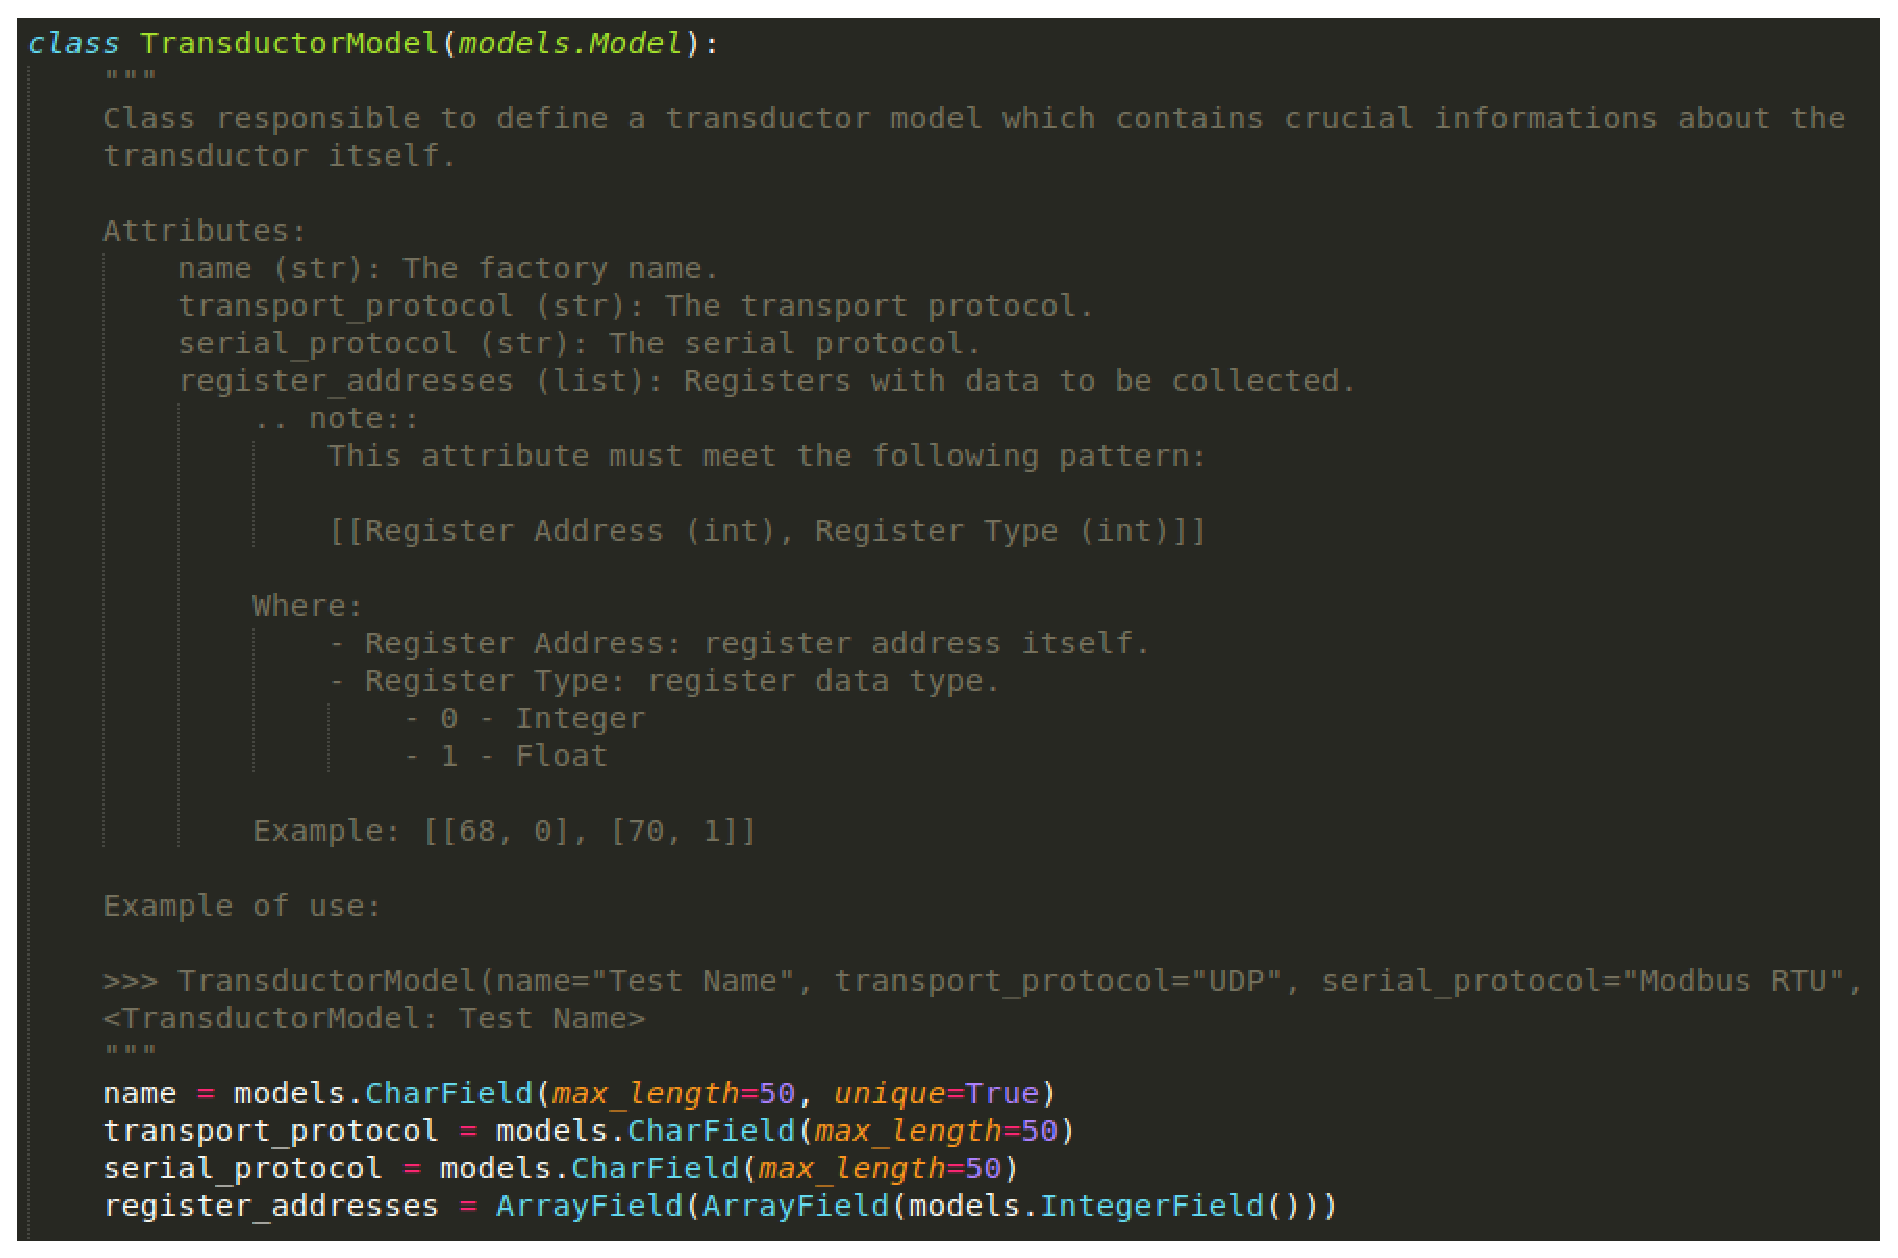
\includegraphics[keepaspectratio=true,scale=0.5]{figuras/documentacao01.eps}
    \caption{Exemplo de Documentação Utilizando \textit{Google Python Style}. Fonte: autor}
    \label{documentacao01}
\end{figure}

A estrutura \textit{Boilerplate}\footnote{\url{https://github.com/fabiommendes/python-boilerplate}} foi adicionada ao projeto com o objetivo de realizar uma melhor estruturação dos módulos e realizar pré-configurações para ambientes de desenvolvimendo/produção, assim como no auxílio para utilização das ferramentas Sphinx e Coverage.

\section{Sprint 05 (19/09/2016 à 30/09/2016) - Refatoração Arquitetural e Protocolo Serial}
Tendo em vista o forte acoplamento gerado pela classe CommunicationProtocol realizou-se uma mudança na arquitetura, onde a classe em questão foi dividia em duas classes abstratas: TransportProtocol e SerialProtocol. A partir dessas classes foram definidas as especializações referentes ao UdpProtol e ModbusRTU, protocolos os quais são utilizados especificamente pelo modelo de transdutor instalado na Universidade. Além dessas mudanças criou-se uma nova classe chamada EnergyOperations, responsável por realizar cálculos matemáticos com os dados de energia coletados. A figura \ref{sprint05arq} ilustra a evolução arquitetural realizado nessa sprint.
\begin{figure}[!htpb]
    \centering
    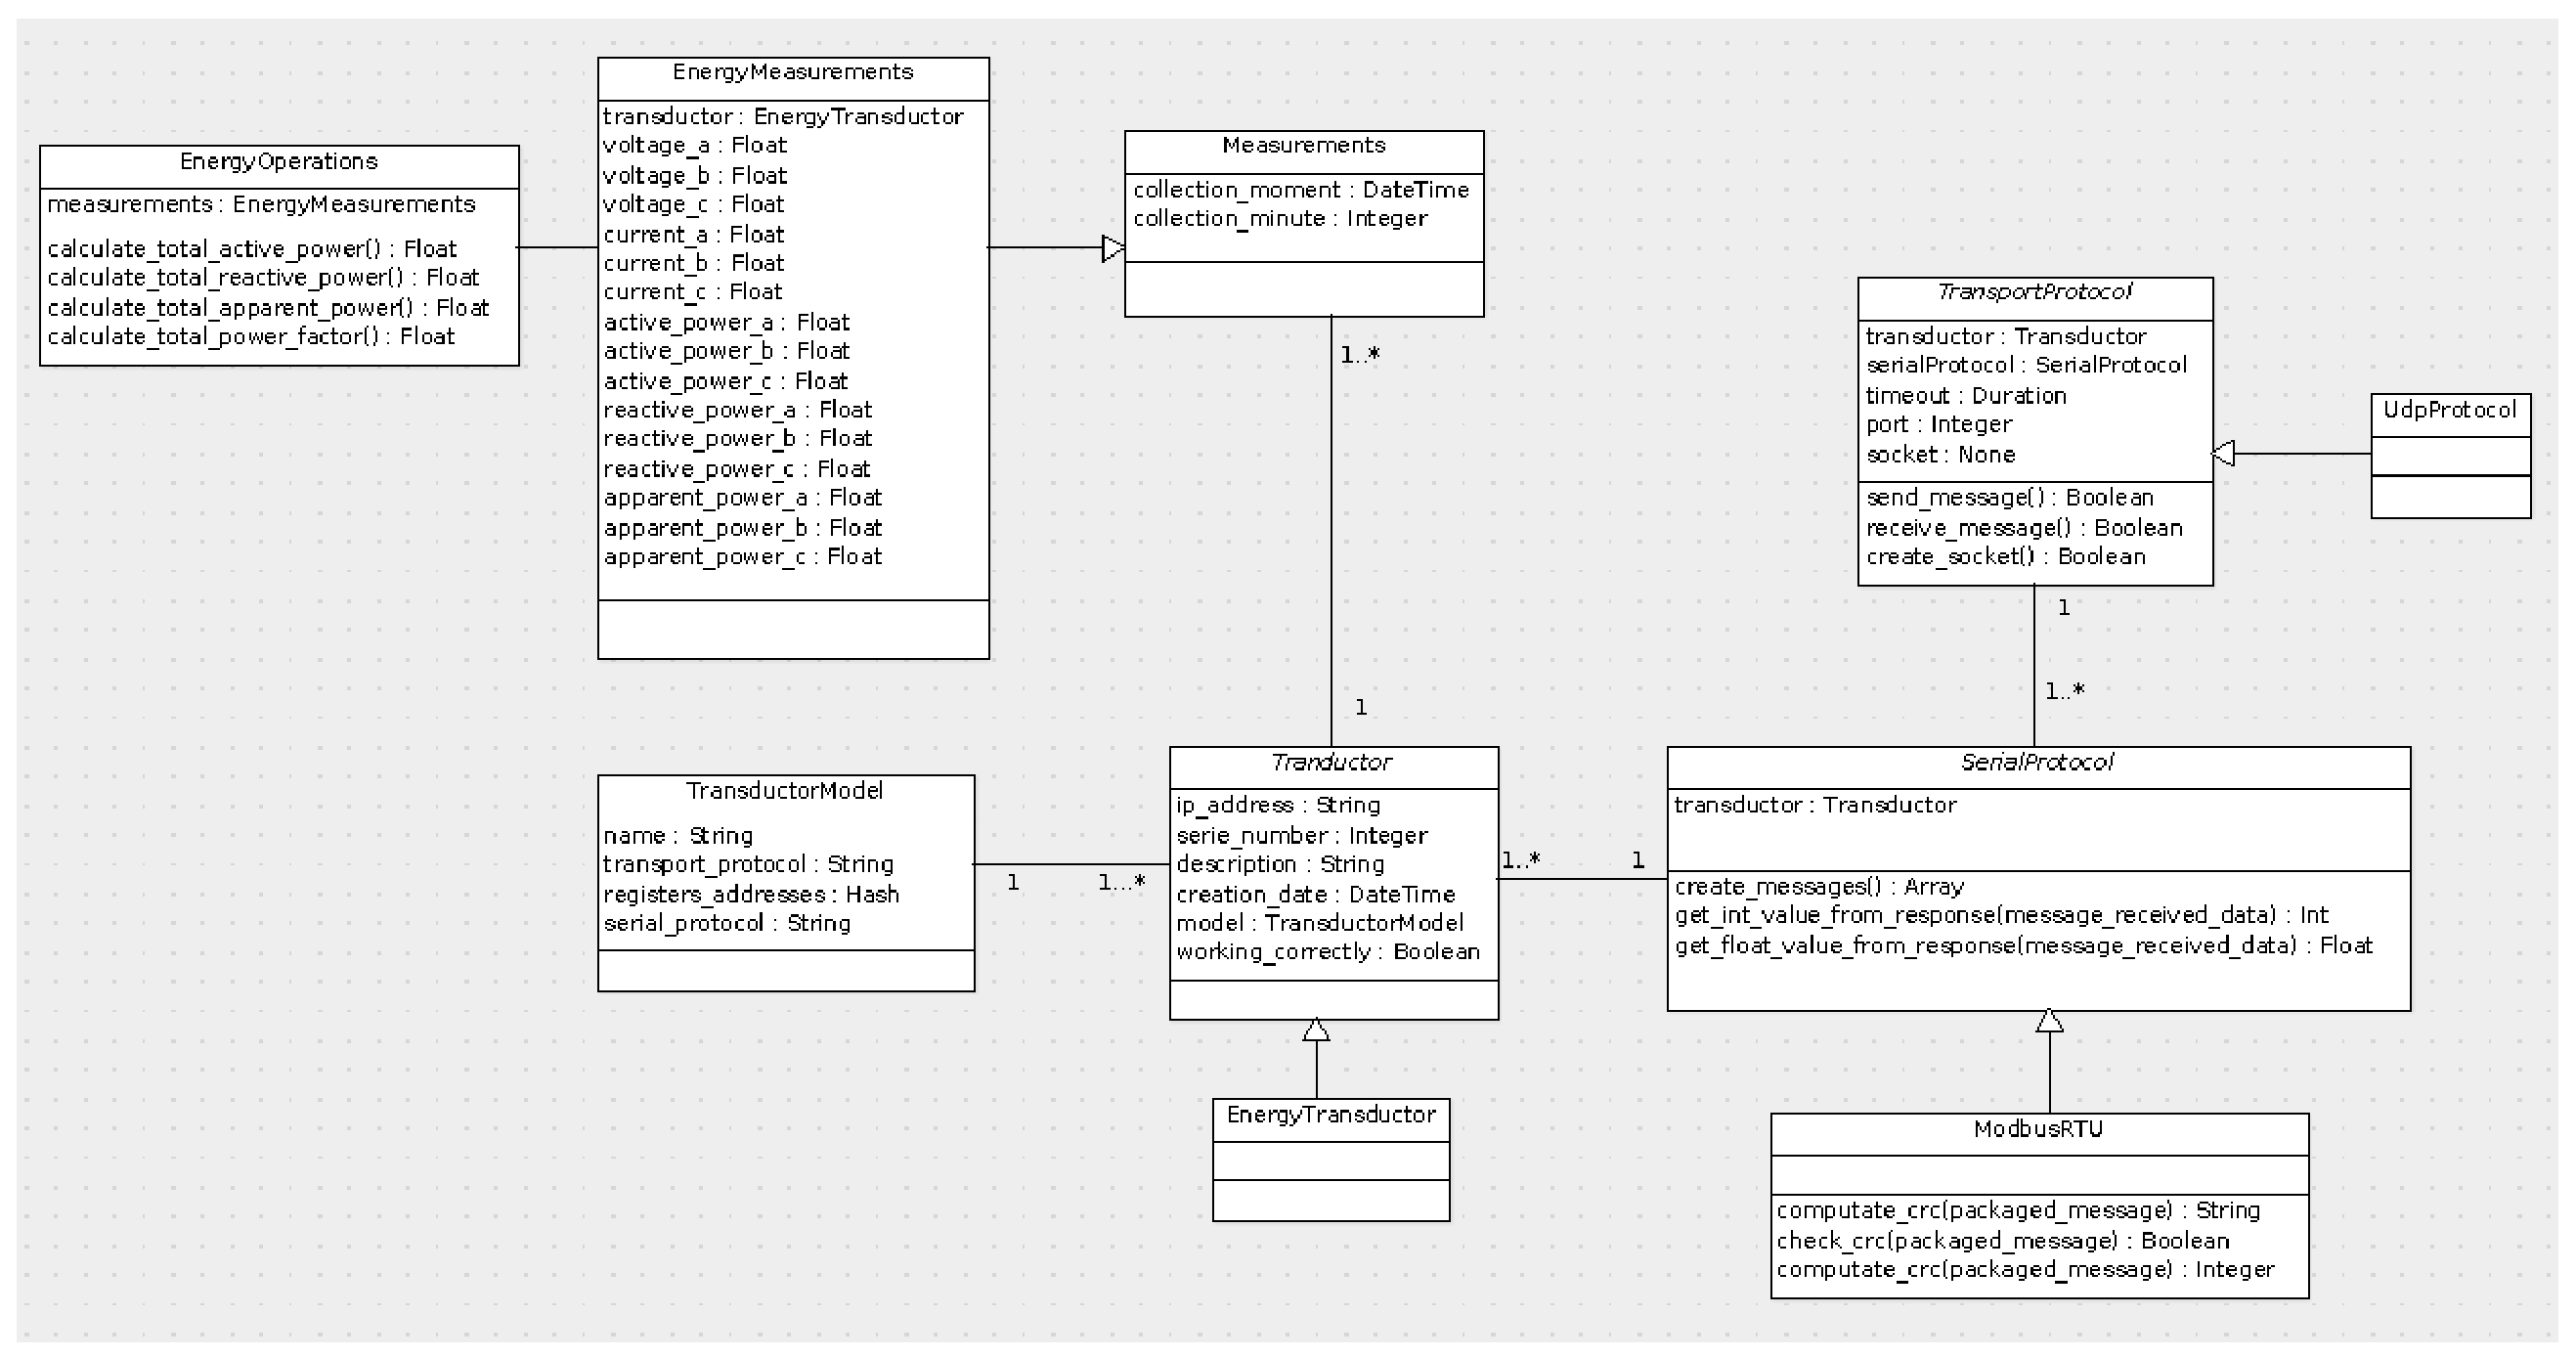
\includegraphics[scale=0.5,angle=90]{figuras/sprint05arq.eps}
    \caption{Arquitetura SME-UnB Sprint 05. Fonte: autor}
    \label{sprint05arq}
\end{figure}

Além das mudanças arquiteturais, foram implementadas e testadas as classes SerialProtocol, ModbusRTU e EnergyOperations. Obteve-se uma cobertura de 96\% ao fim da sprint, conforme ilustrado na figura \ref{cobertura02}.
\begin{figure}[!htpb]
    \centering
    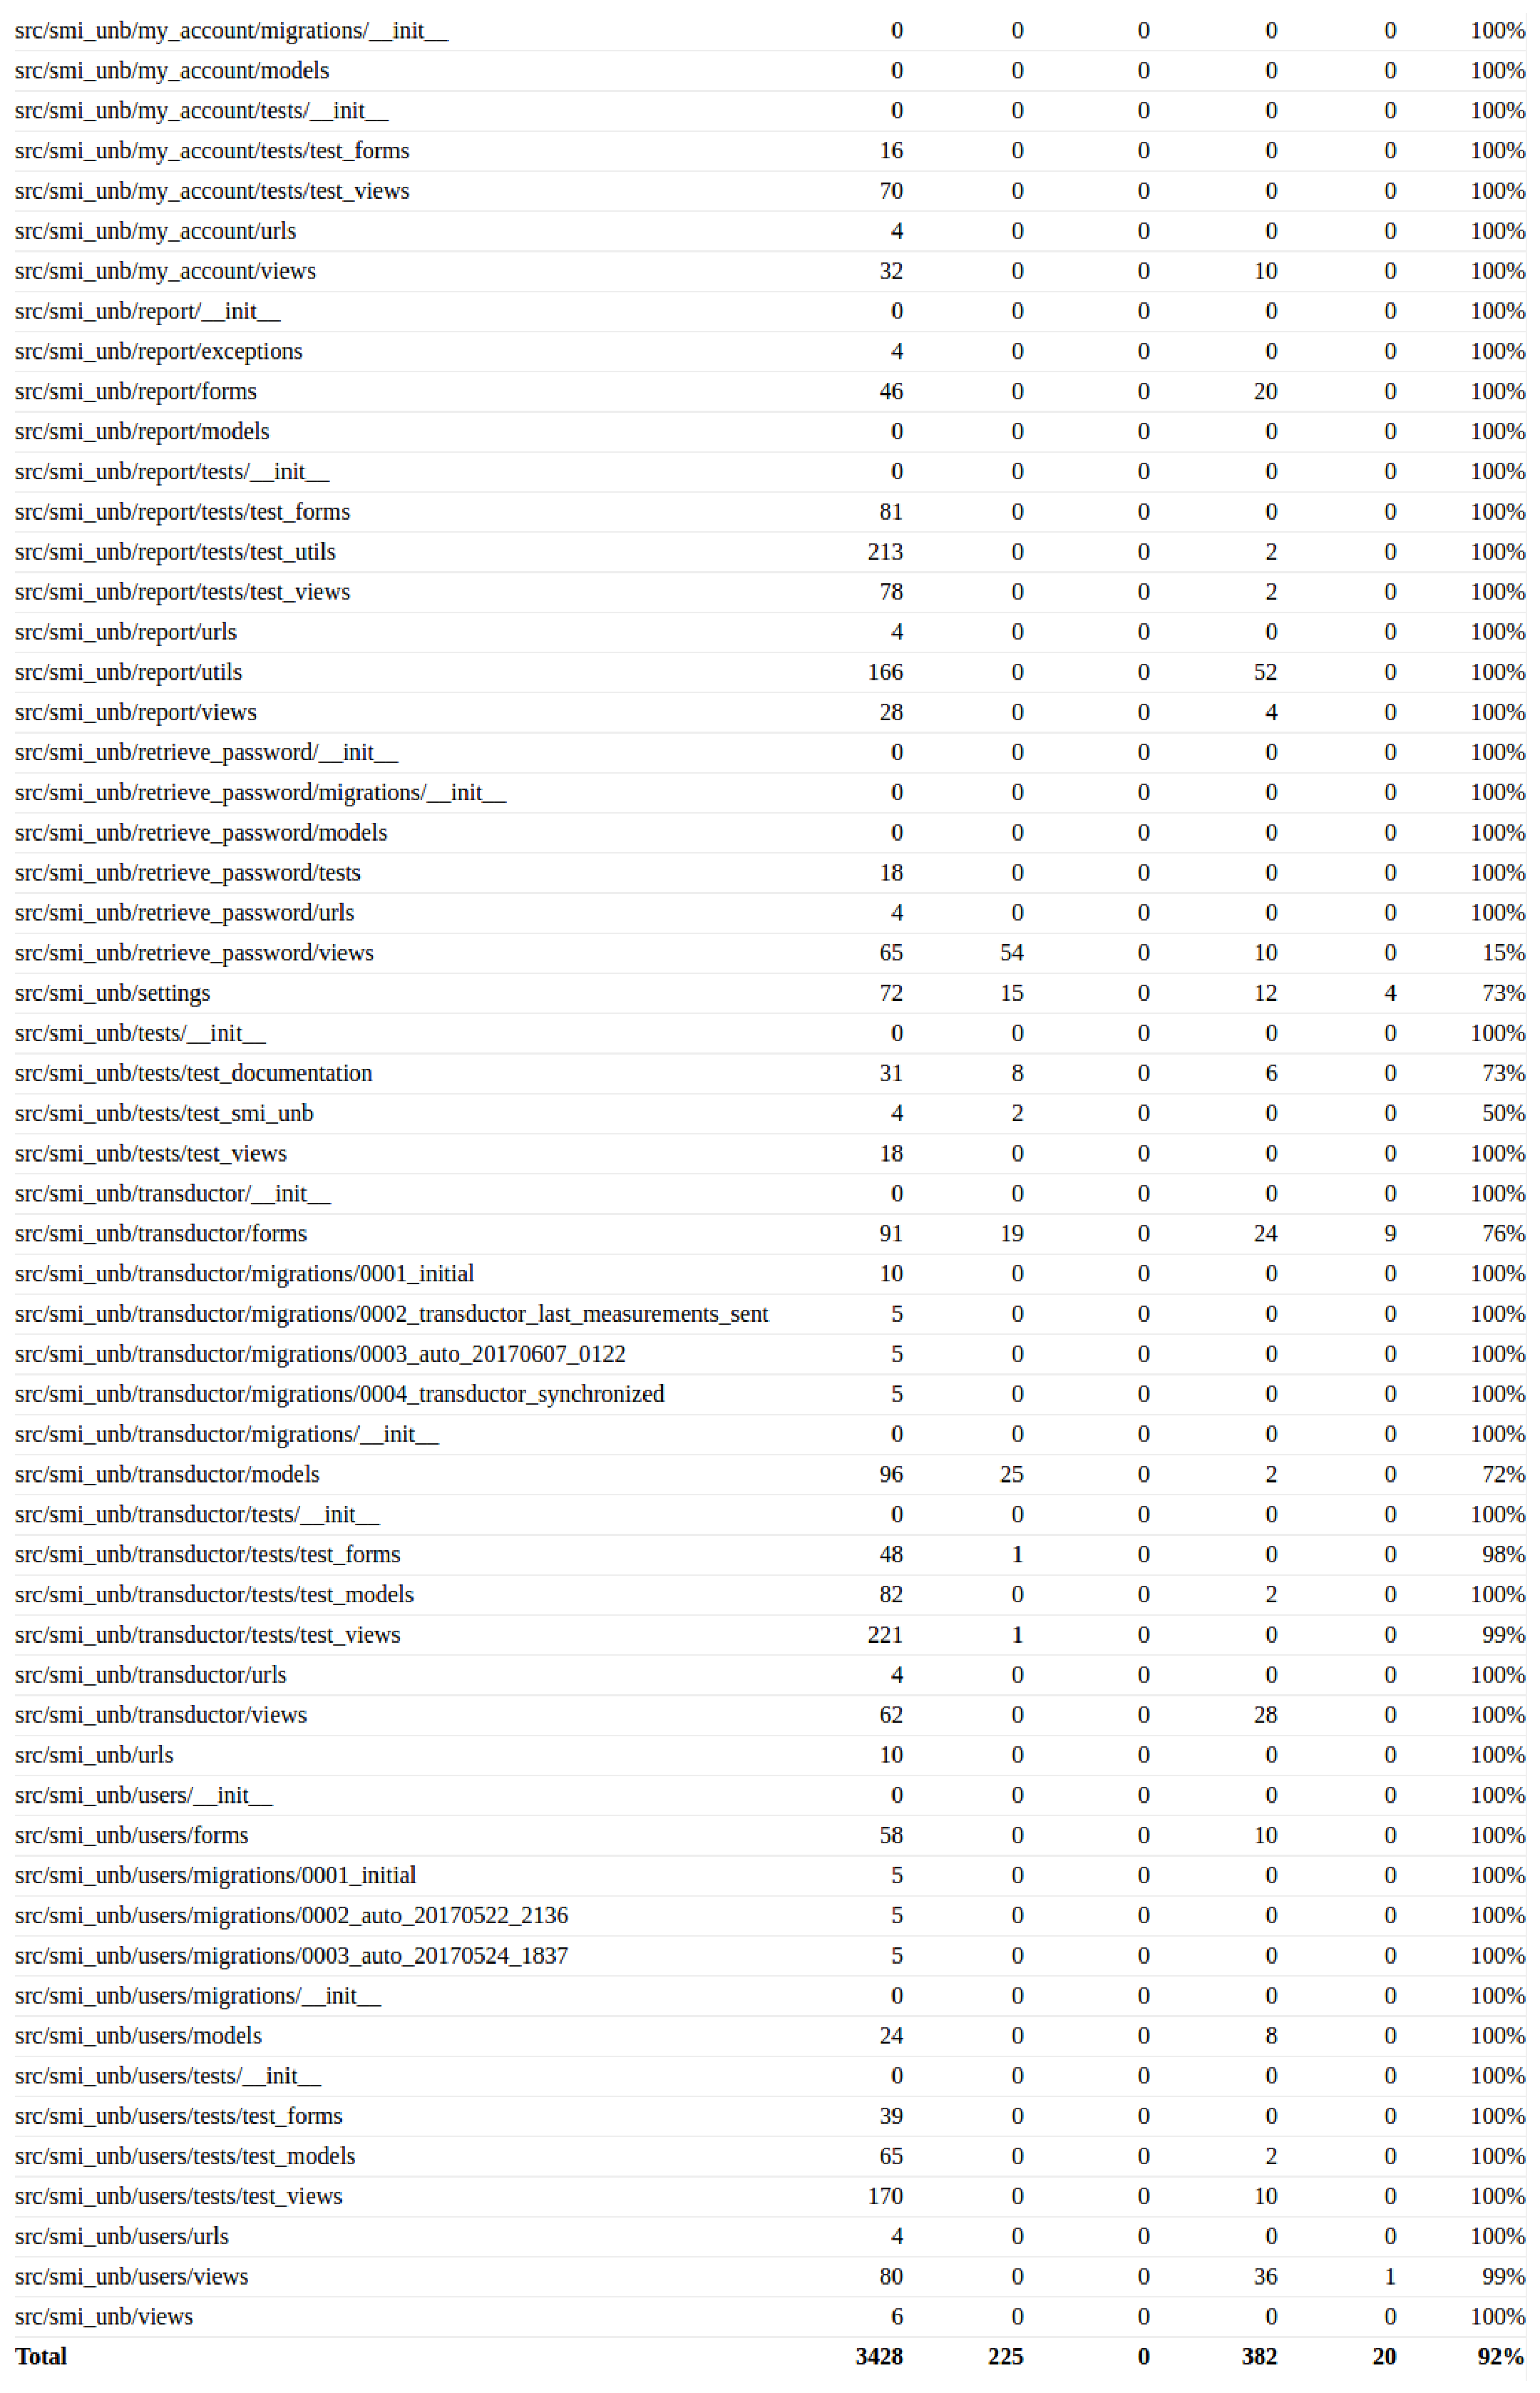
\includegraphics[keepaspectratio=true,scale=0.6]{figuras/cobertura02.eps}
    \caption{Cobertura Total de Código Sprint 05. Fonte: autor}
    \label{cobertura02}
\end{figure}

\section{Sprint 06 (03/10/2016 à 14/10/2016) - Protocolo de Transporte e Testes com Mock}
Após implementado o protocolo serial, realizou-se o desenvolvimento do protocolo de transporte. Sua principal função é comunicar-se com o transdutor utilizando o protocolo utilizado pelo mesmo e tratar as questões referentes à \textit{timeout} e tentativas consecutivas de envio de requisições. Além disso, foram refatorados os testes do sistema utilizando \textit{Mocks}\footnote{\url{https://docs.python.org/3/library/unittest.mock.html}}, objetivando maior desempenho e efetivamente testar unitariamente os métodos. A figura \ref{exemplo_mock} ilustra um exemplo de teste da classe UdpProtocol utilizando \textit{Mock}. A cobertura de código, figura \ref{cobertura03}, não se alterou comparado à sprint anterior.

\begin{figure}[!htpb]
    \centering
    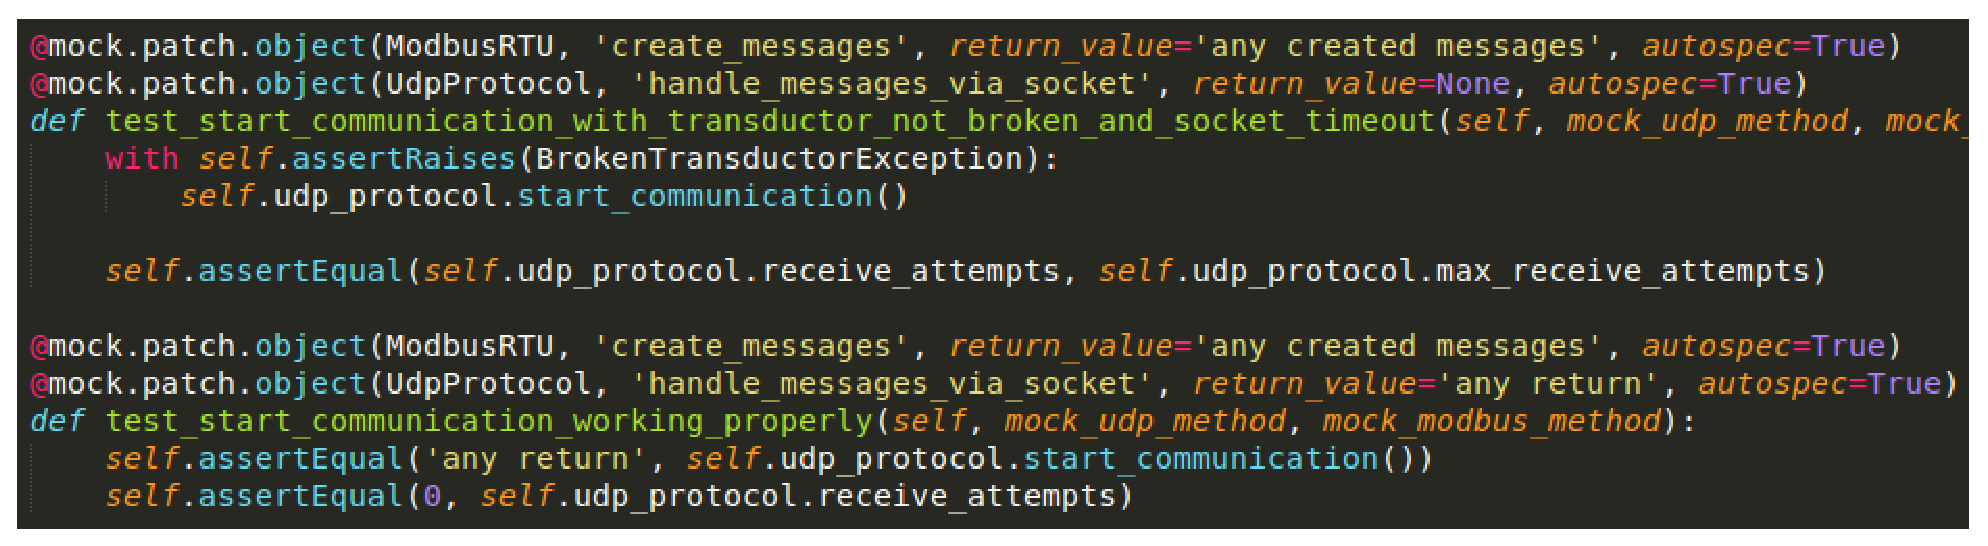
\includegraphics[keepaspectratio=true,scale=0.5]{figuras/exemplo_mock.eps}
    \caption{Exemplo de Teste utilizando \textit{Mock}. Fonte: autor}
    \label{exemplo_mock}
\end{figure}

\begin{figure}[!htpb]
    \centering
    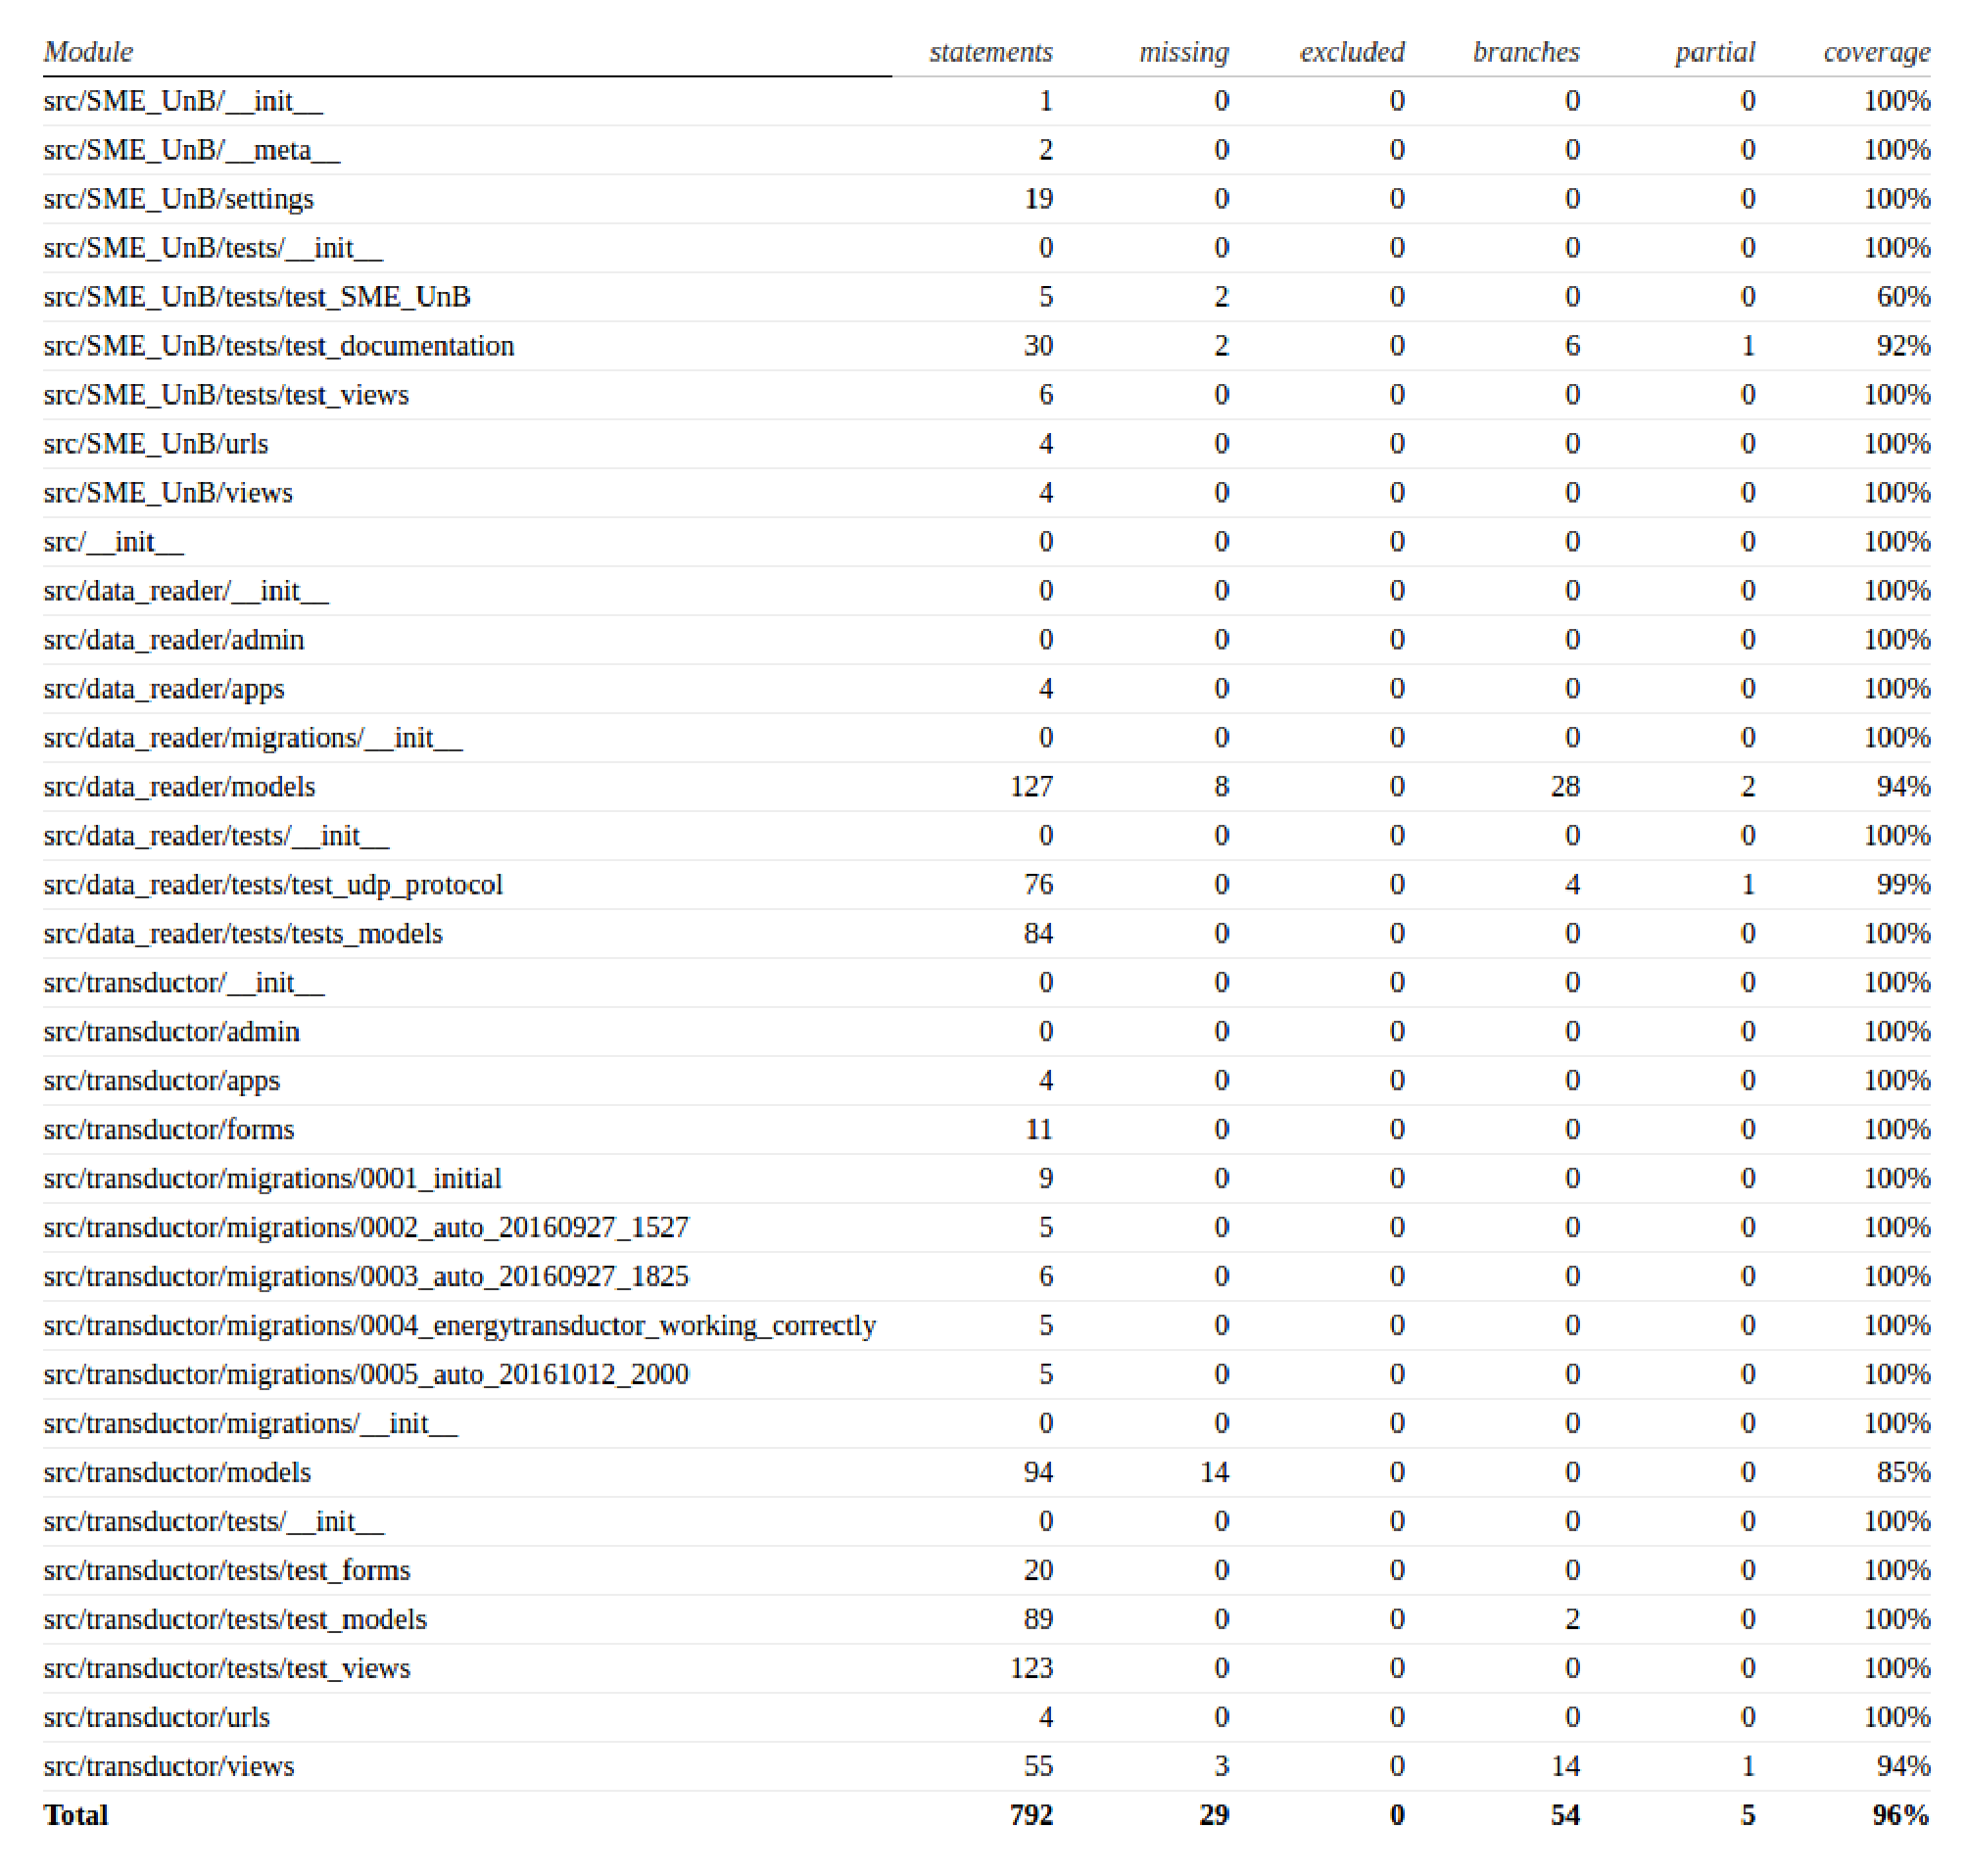
\includegraphics[keepaspectratio=true,scale=0.5]{figuras/cobertura03.eps}
    \caption{Cobertura Total de Código Sprint 06. Fonte: autor}
    \label{cobertura03}
\end{figure}

\section{Sprint 07 (17/10/2016 à 28/10/2016)}
Após implementar os protocolos de tranporte e serial verificou-se a necessidade de uma classe que realizasse toda a comunicação dos mesmos, ou seja, desempenhasse a coleta das medições de cada transdutor. Essa classe foi definida como DataCollector e utiliza os princípios de \textit{threads}\footnote{\url{https://docs.python.org/2/library/threading.html}} para inicar ``simultaneamente'' a coleta de dados de todos os trandutores. A figura \ref{sprint07arq} ilustra a nova arquitetura gerada.

\begin{figure}[!htpb]
    \centering
    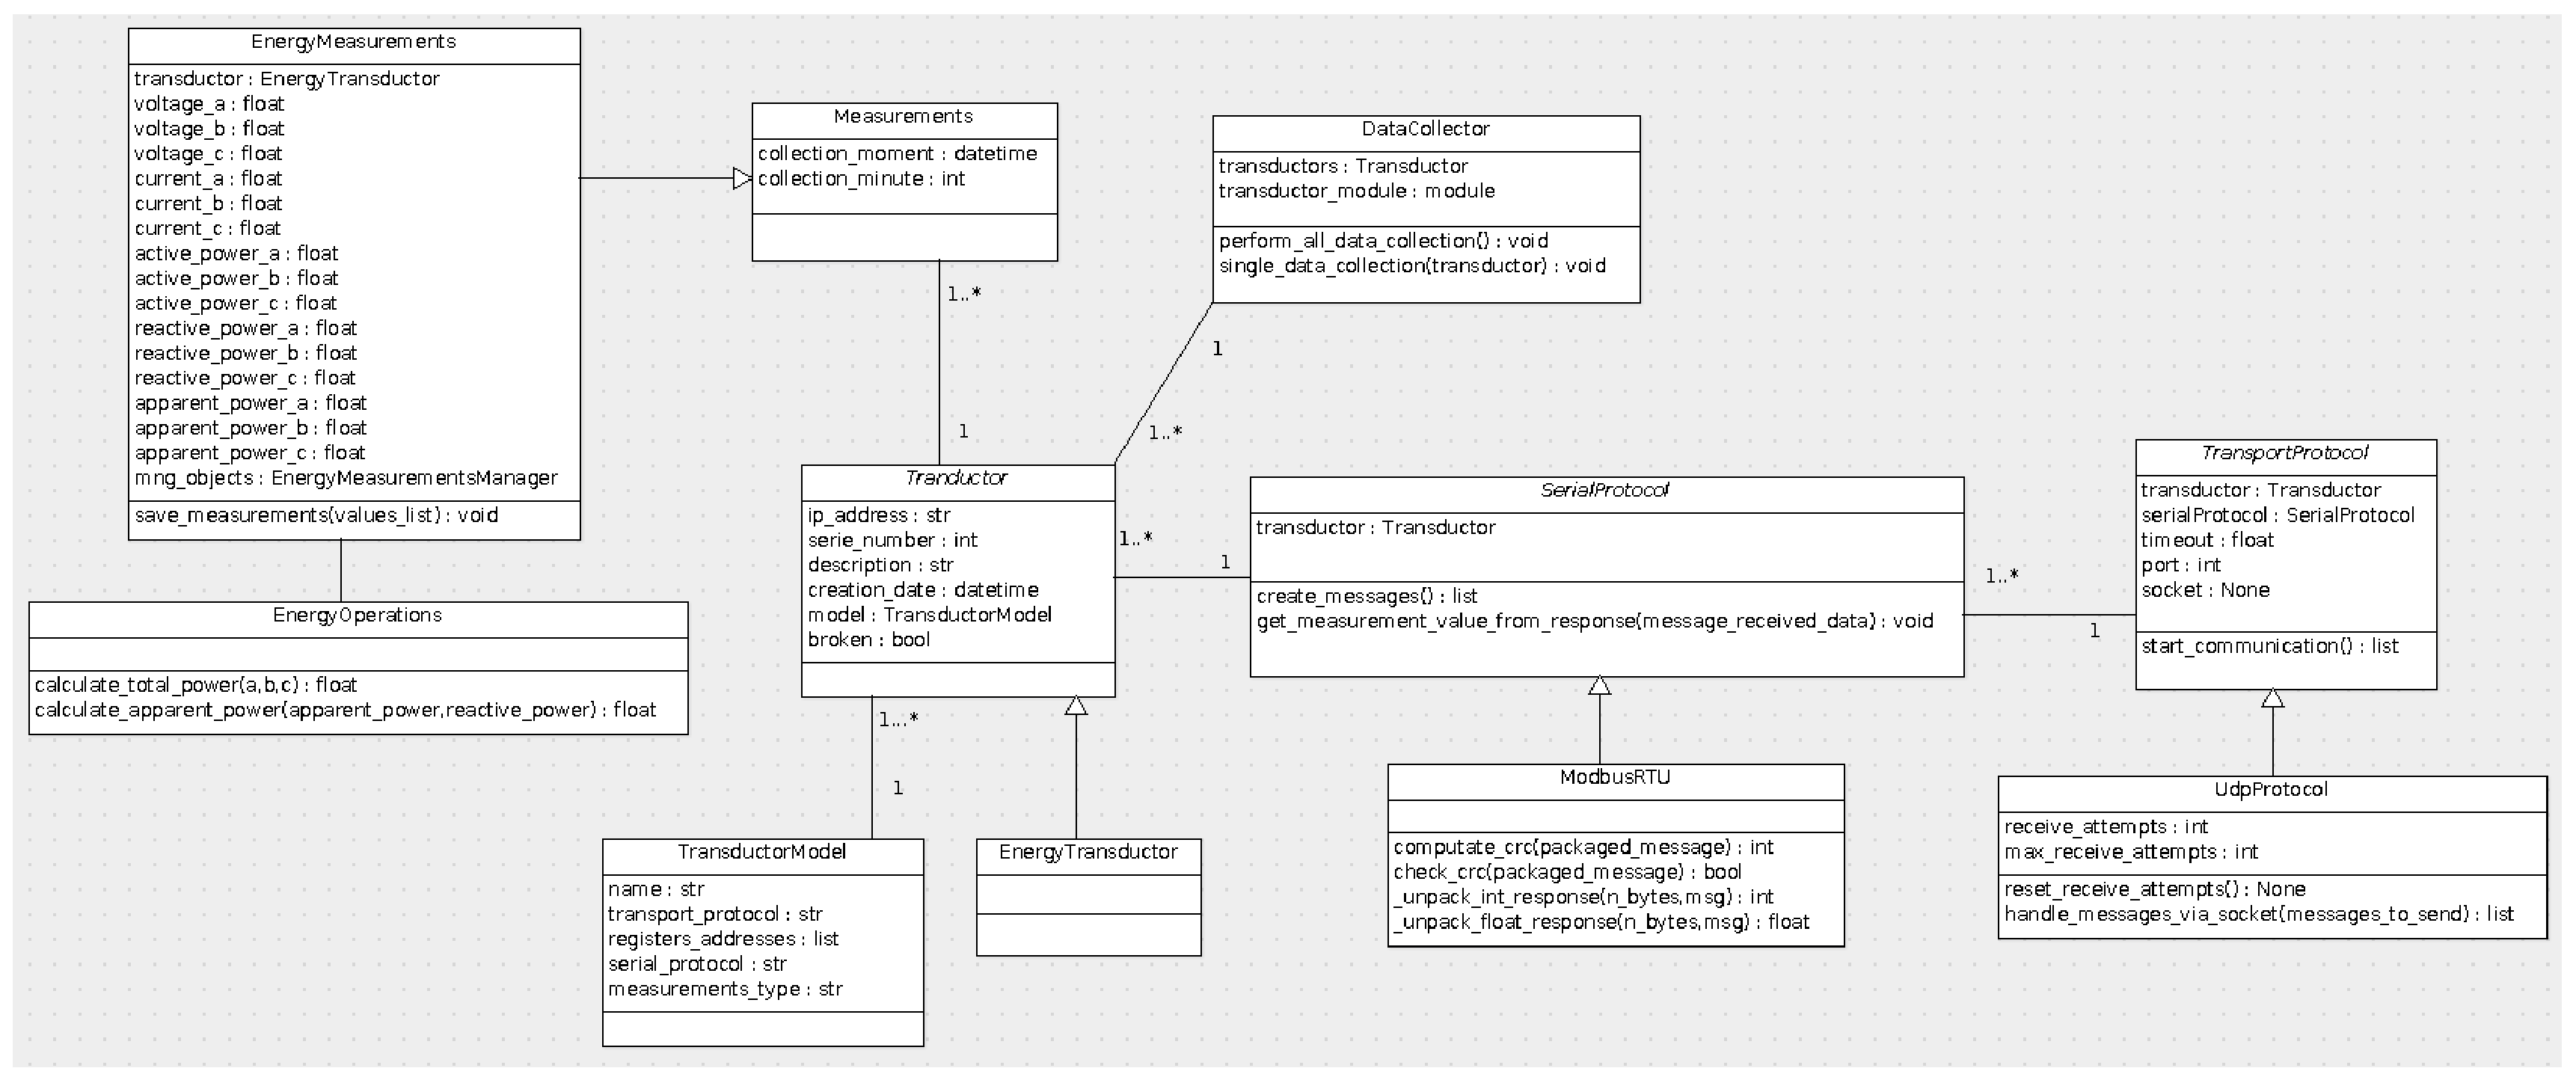
\includegraphics[scale=0.4,angle=90]{figuras/sprint07arq.eps}
    \caption{Arquitetura SME-UnB Sprint 07. Fonte: autor}
    \label{sprint07arq}
\end{figure}

\section{Sprint 08}


\bookmarksetup{startatroot}

\postextual

\bibliography{bibliografia}
%\begin{apendicesenv}

\partapendices

\chapter{Integração Contínua}
\begin{python}[caption={\textit{Log} de integração contínua do SMI-UnB}, captionpos=b, label={integracao_cont}]
Running with gitlab-ci-multi-runner 9.3.0-rc.2 (110d530)
  on docker-auto-scale (e11ae361)
Using Docker executor with image python:3.5 ...
Starting service postgres:latest ...
Pulling docker image postgres:latest ...
Using docker image postgres:latest for postgres service...
Waiting for services to be up and running...
Using docker image sha256 for predefined container...
Pulling docker image python:3.5 ...
Using docker image python:3.5 for build container...
Running on runner-e11ae361-project-1216906...
Cloning repository...
Cloning into '/builds/brenddongontijo/SMI-UnB'...
Checking out e70a256f as master...
Skipping Git submodules setup
$ apt-get update -qq
$ apt-get install python3-pip -y -qq
# Installing packages...
$ flake8 src/ --exclude migrations
$ coverage run manage.py test \
smi_unb --settings=smi_unb.settings_runner
# Running tests...
----------------------------------------------
Ran 192 tests in 17.081s
OK
Creating a new SECRET_KEY at security/secret_key.dat
Running server in DEBUG mode. Plese do *not* go to production!
Documentation files not found: disabling tests!
Creating test database for alias 'default'...
Destroying test database for alias 'default'...
$ coverage report
# Coverage report...
Job succeeded
\end{python}

\chapter{Cobertura Total de Código}
\begin{figure}[!htpb]
    \centering
    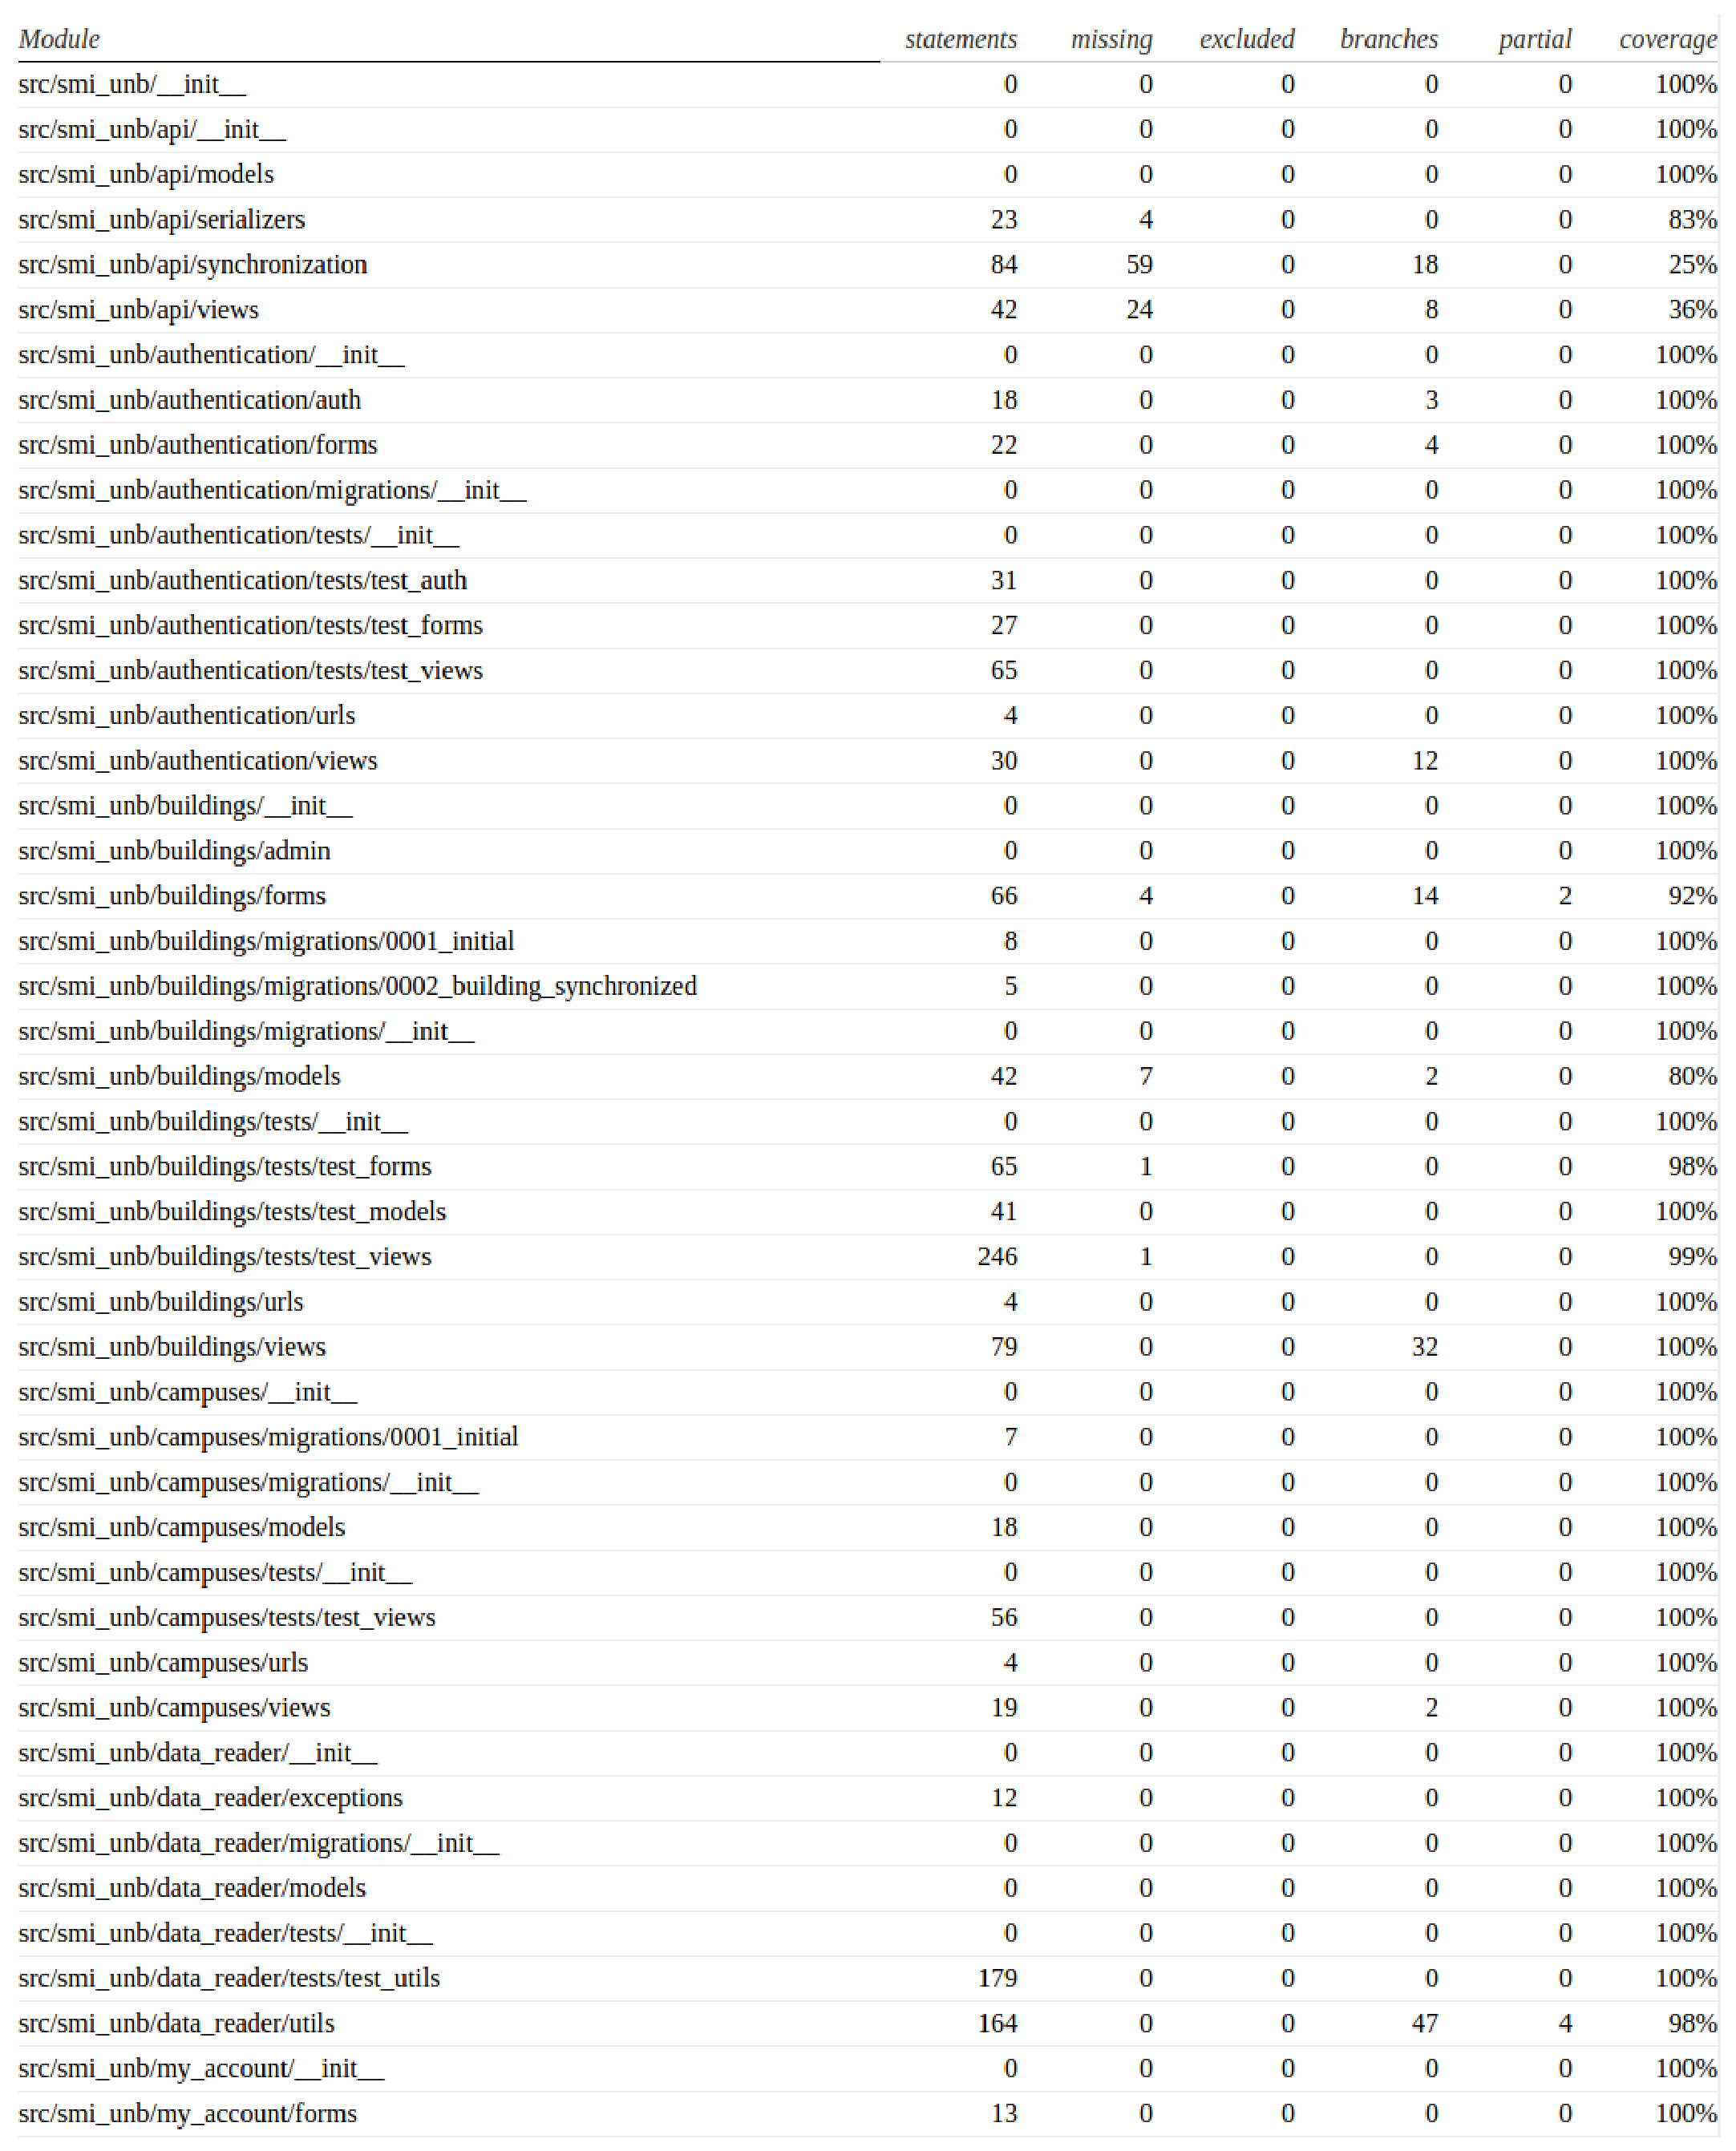
\includegraphics[keepaspectratio=true,scale=0.45]{figuras/cobertura01.eps}
    \caption{Primeira parte da cobertura do SMI-UnB.}
    \label{cobertura01}
\end{figure}

\begin{figure}[!htpb]
    \centering
    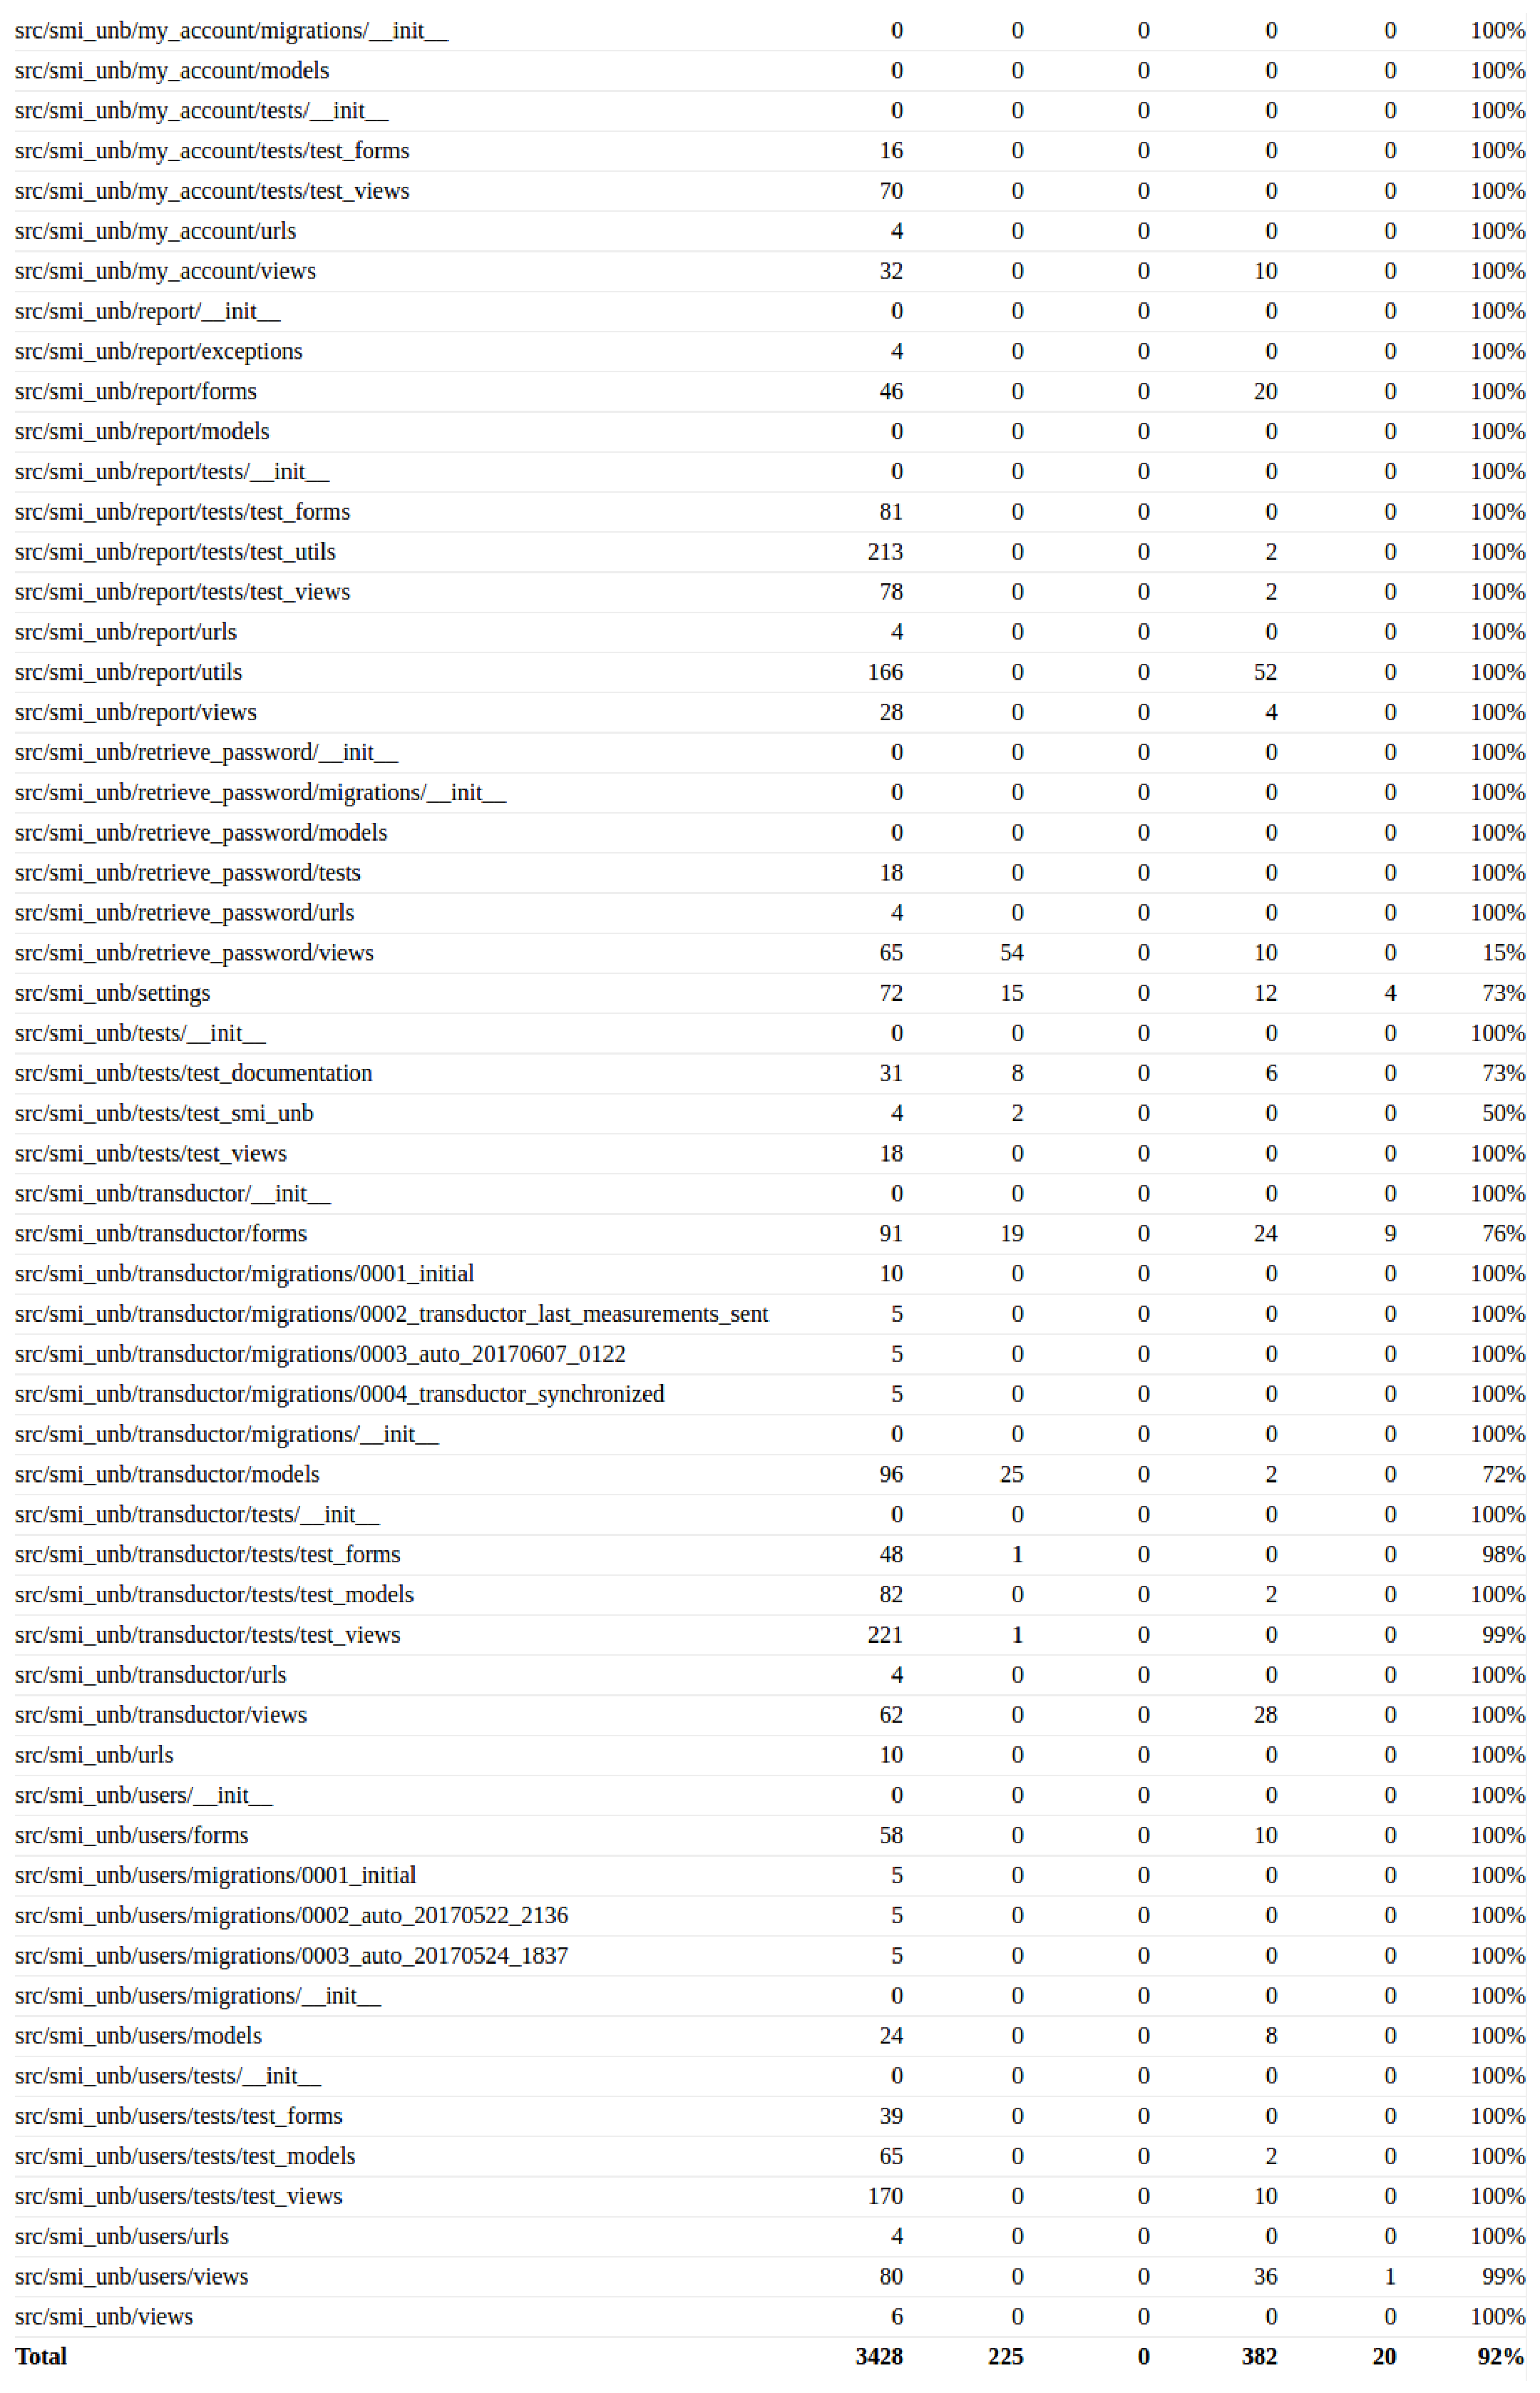
\includegraphics[keepaspectratio=true,scale=0.45]{figuras/cobertura02.eps}
    \caption{Segunda parte da cobertura do SMI-UnB.}
    \label{cobertura02}
\end{figure}

\chapter{Imagens da Aplicação}
\begin{figure}[!htpb]
    \centering
    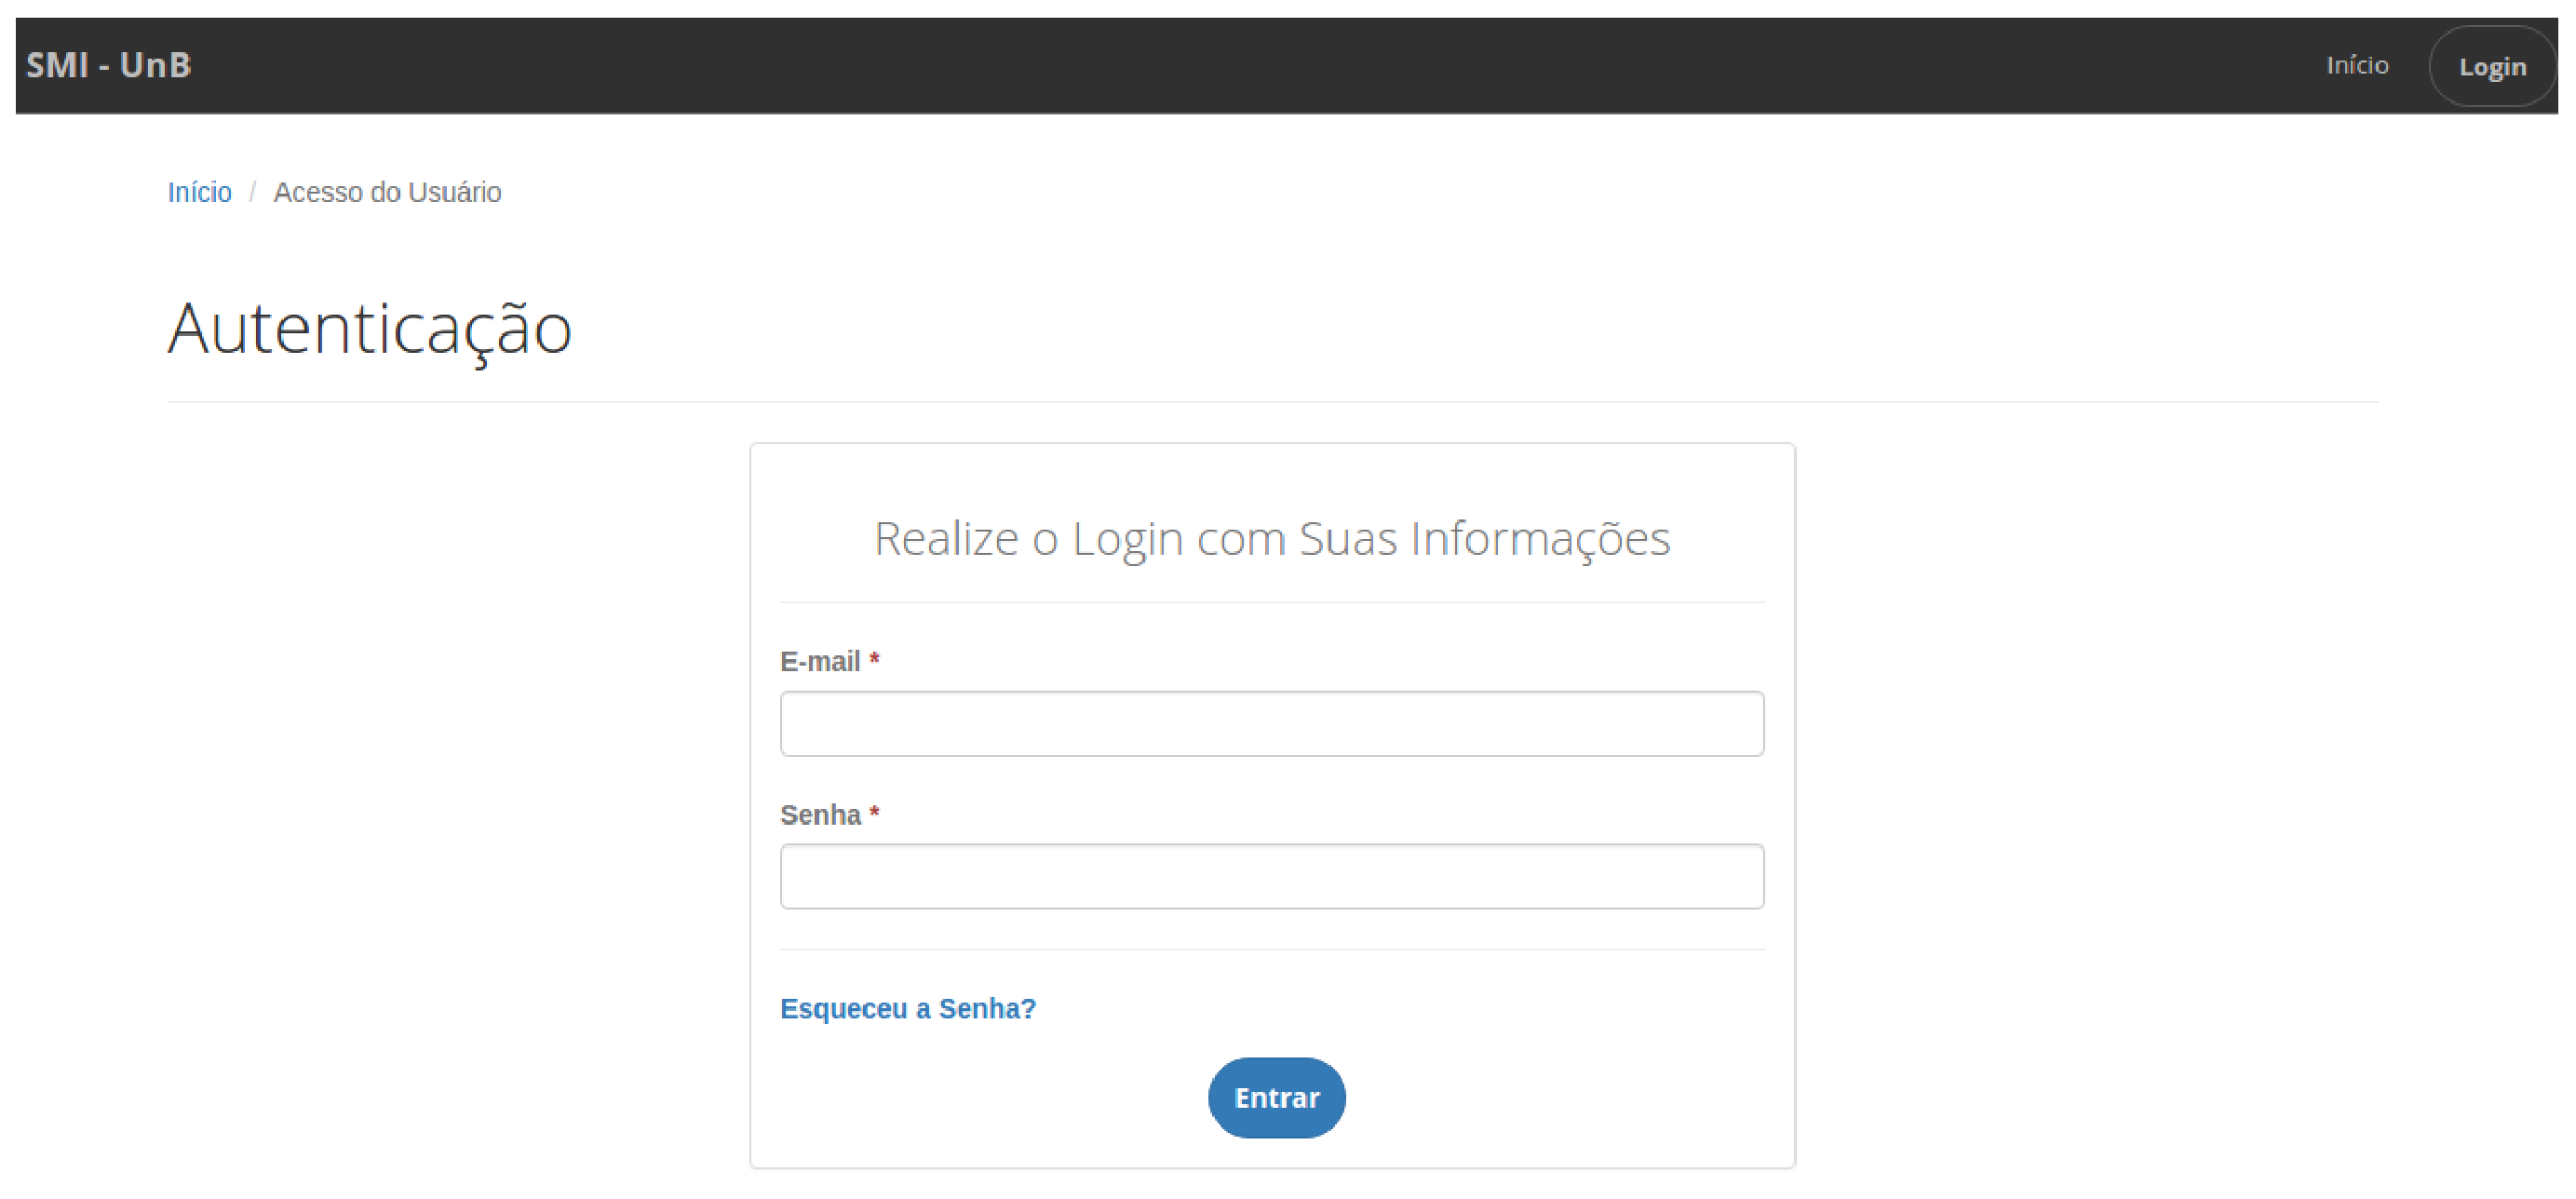
\includegraphics[keepaspectratio=true,scale=0.35]{figuras/img1.eps}
    \caption{Página de autenticação.}
    \label{img1}
\end{figure}

\begin{figure}[!htpb]
    \centering
    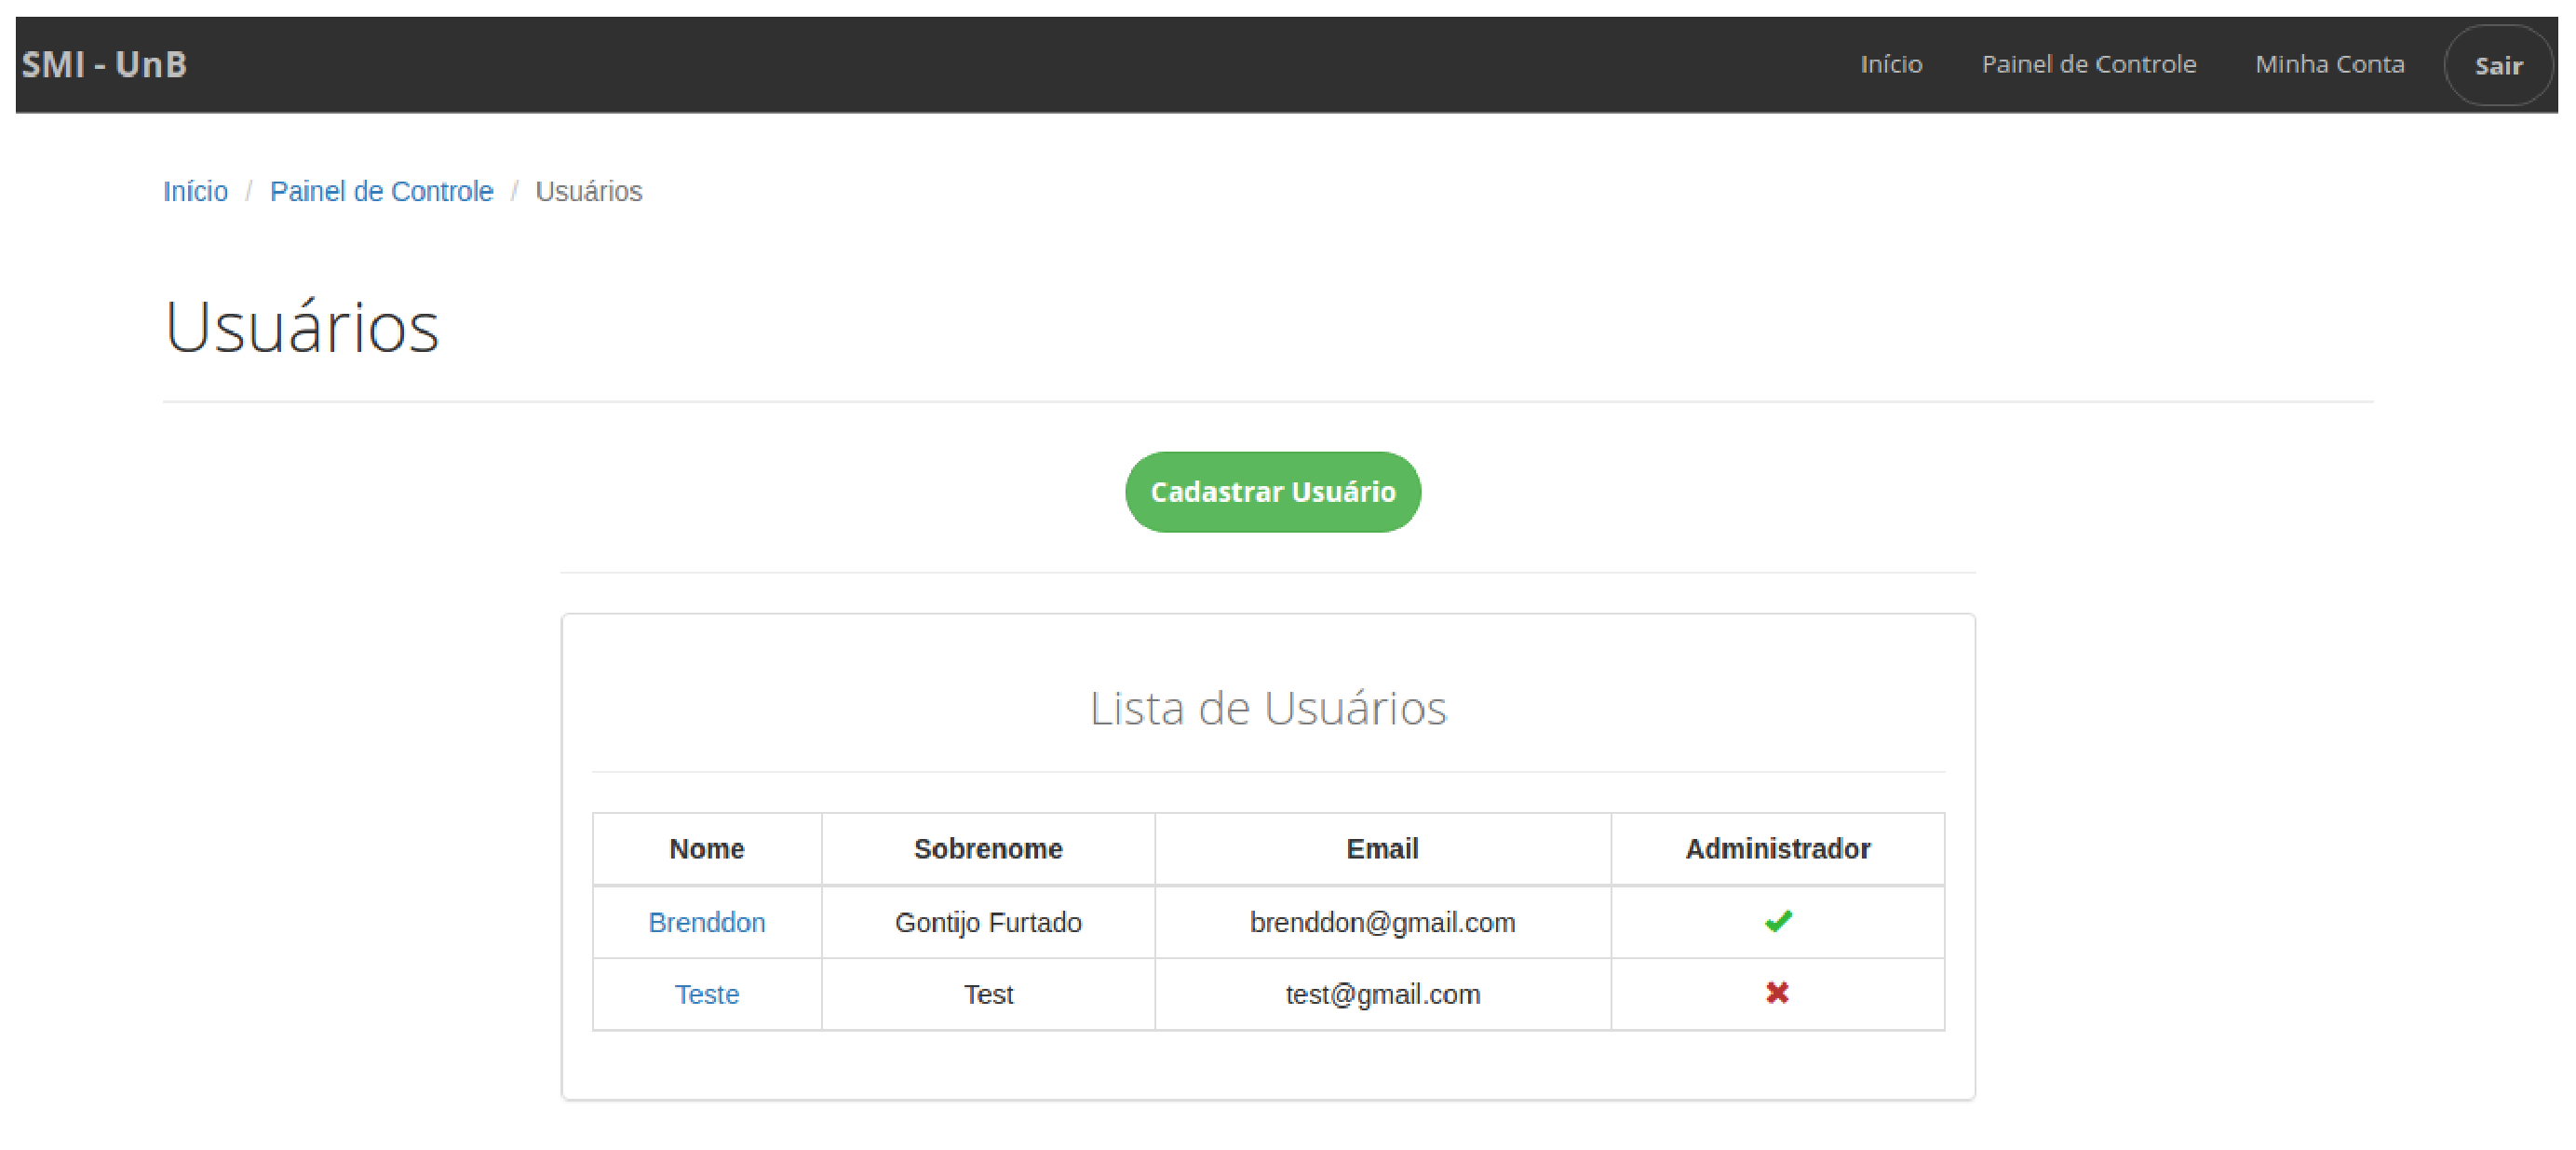
\includegraphics[keepaspectratio=true,scale=0.35]{figuras/img2.eps}
    \caption{Página de usuários.}
    \label{img2}
\end{figure}

\begin{figure}[!htpb]
    \centering
    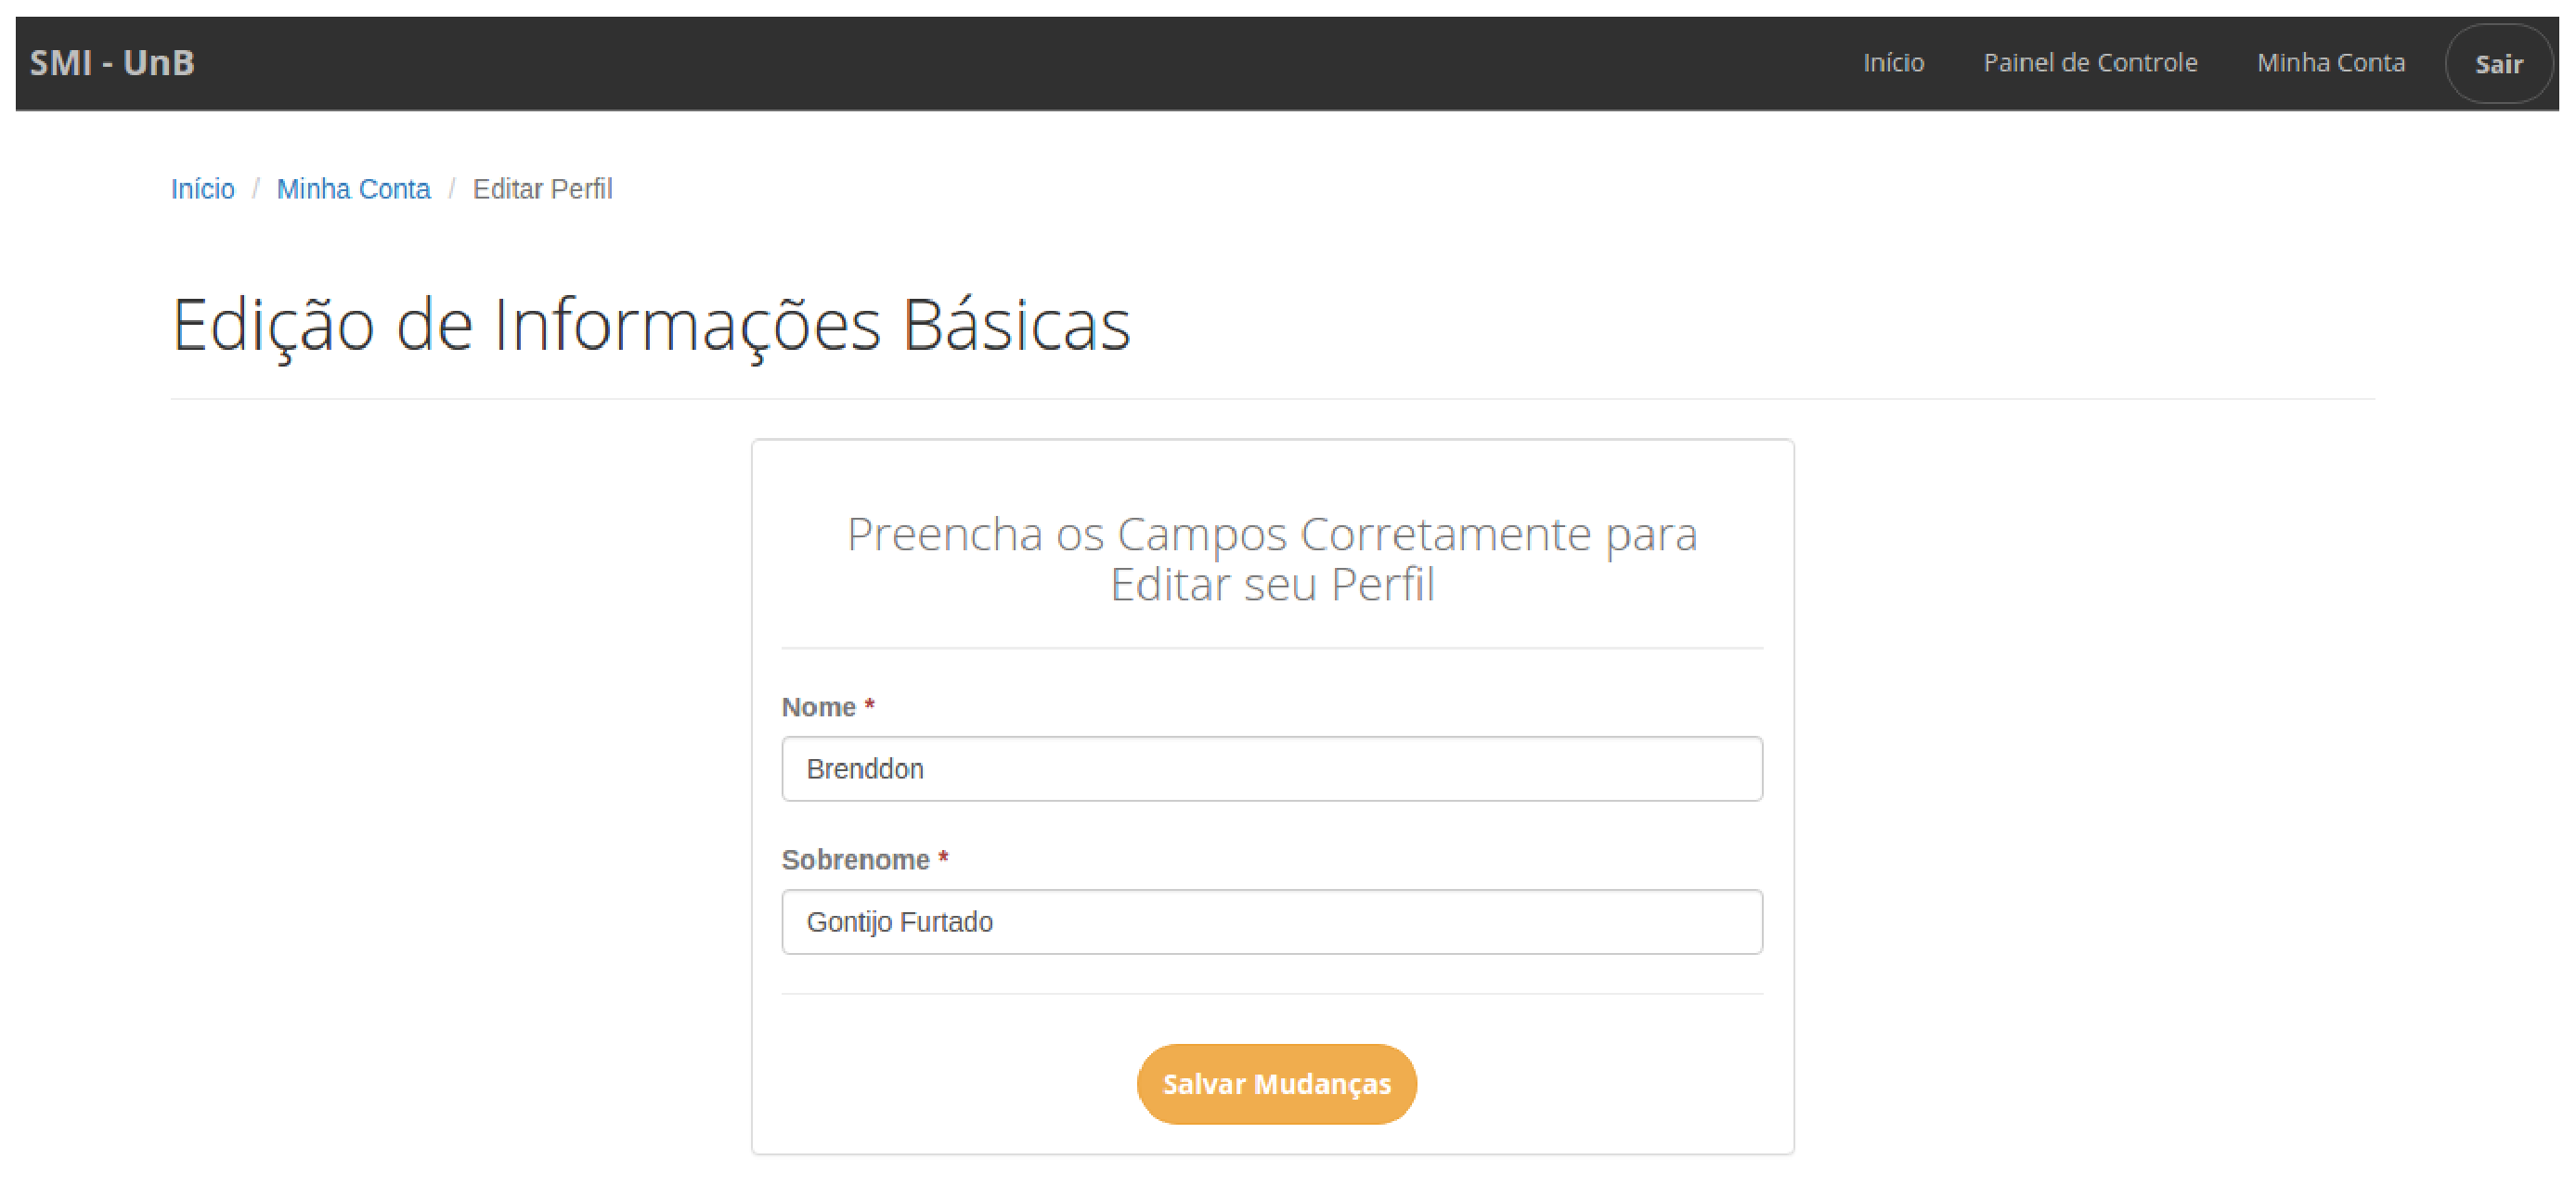
\includegraphics[keepaspectratio=true,scale=0.35]{figuras/img5.eps}
    \caption{Página de edição das informações básicas da conta.}
    \label{img5}
\end{figure}

\begin{figure}[!htpb]
    \centering
    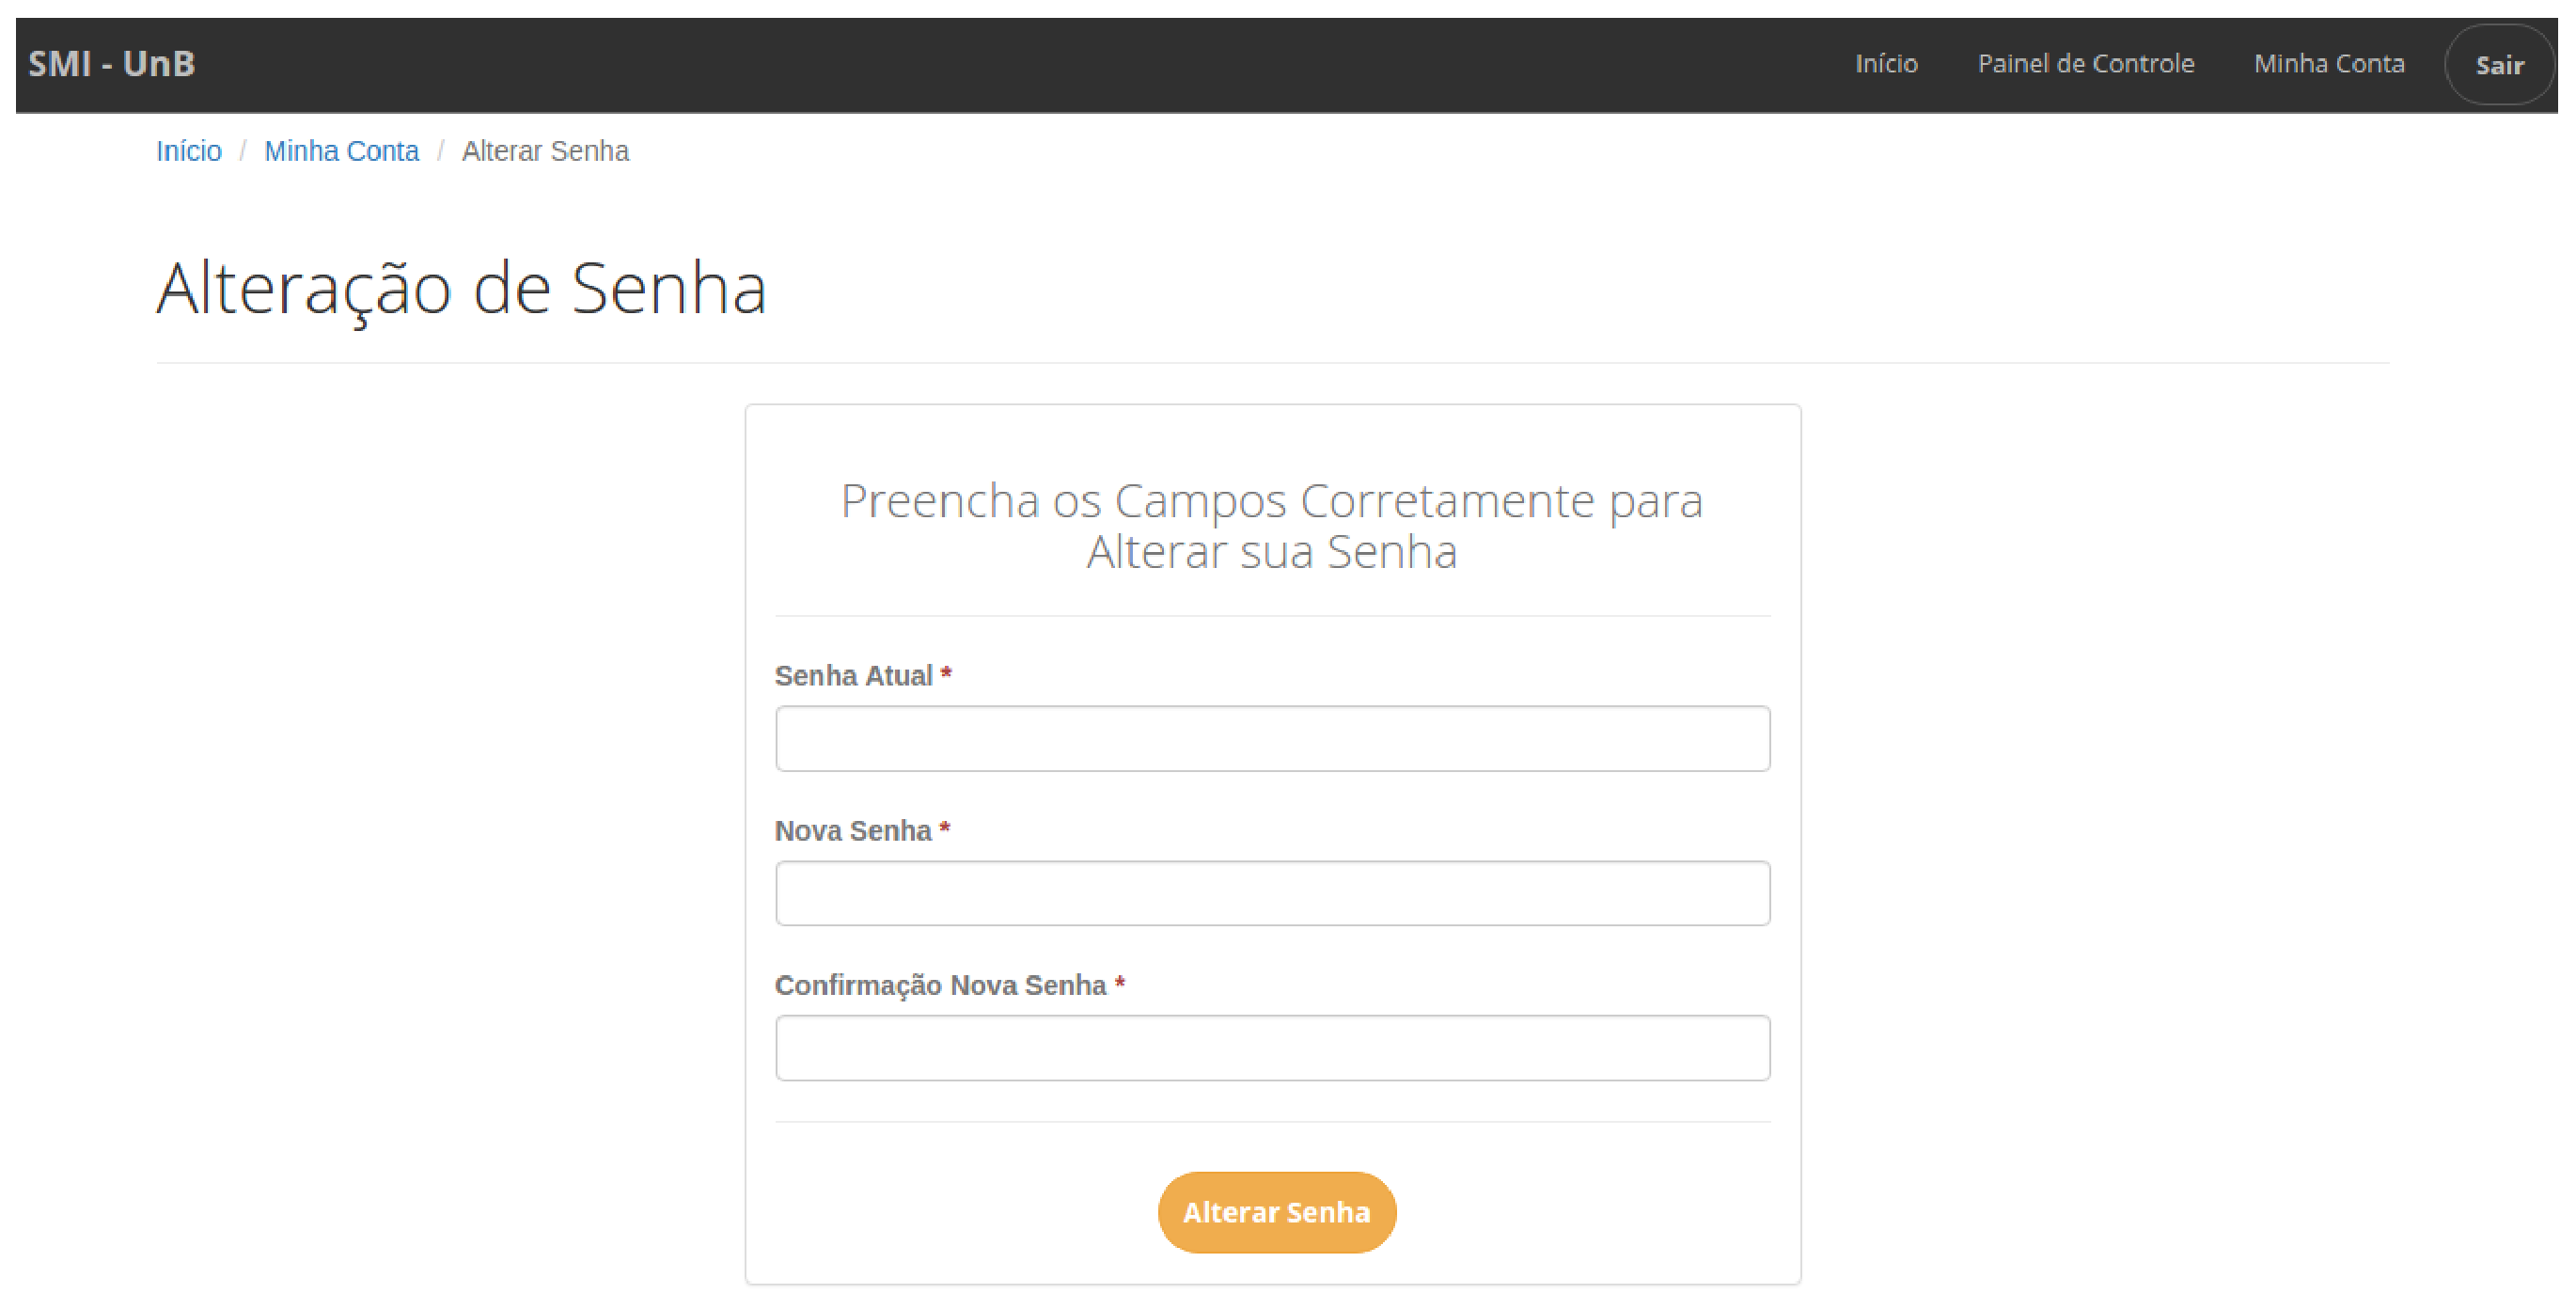
\includegraphics[keepaspectratio=true,scale=0.35]{figuras/img6.eps}
    \caption{Página de alteração de senha.}
    \label{img6}
\end{figure}

\begin{figure}[!htpb]
    \centering
    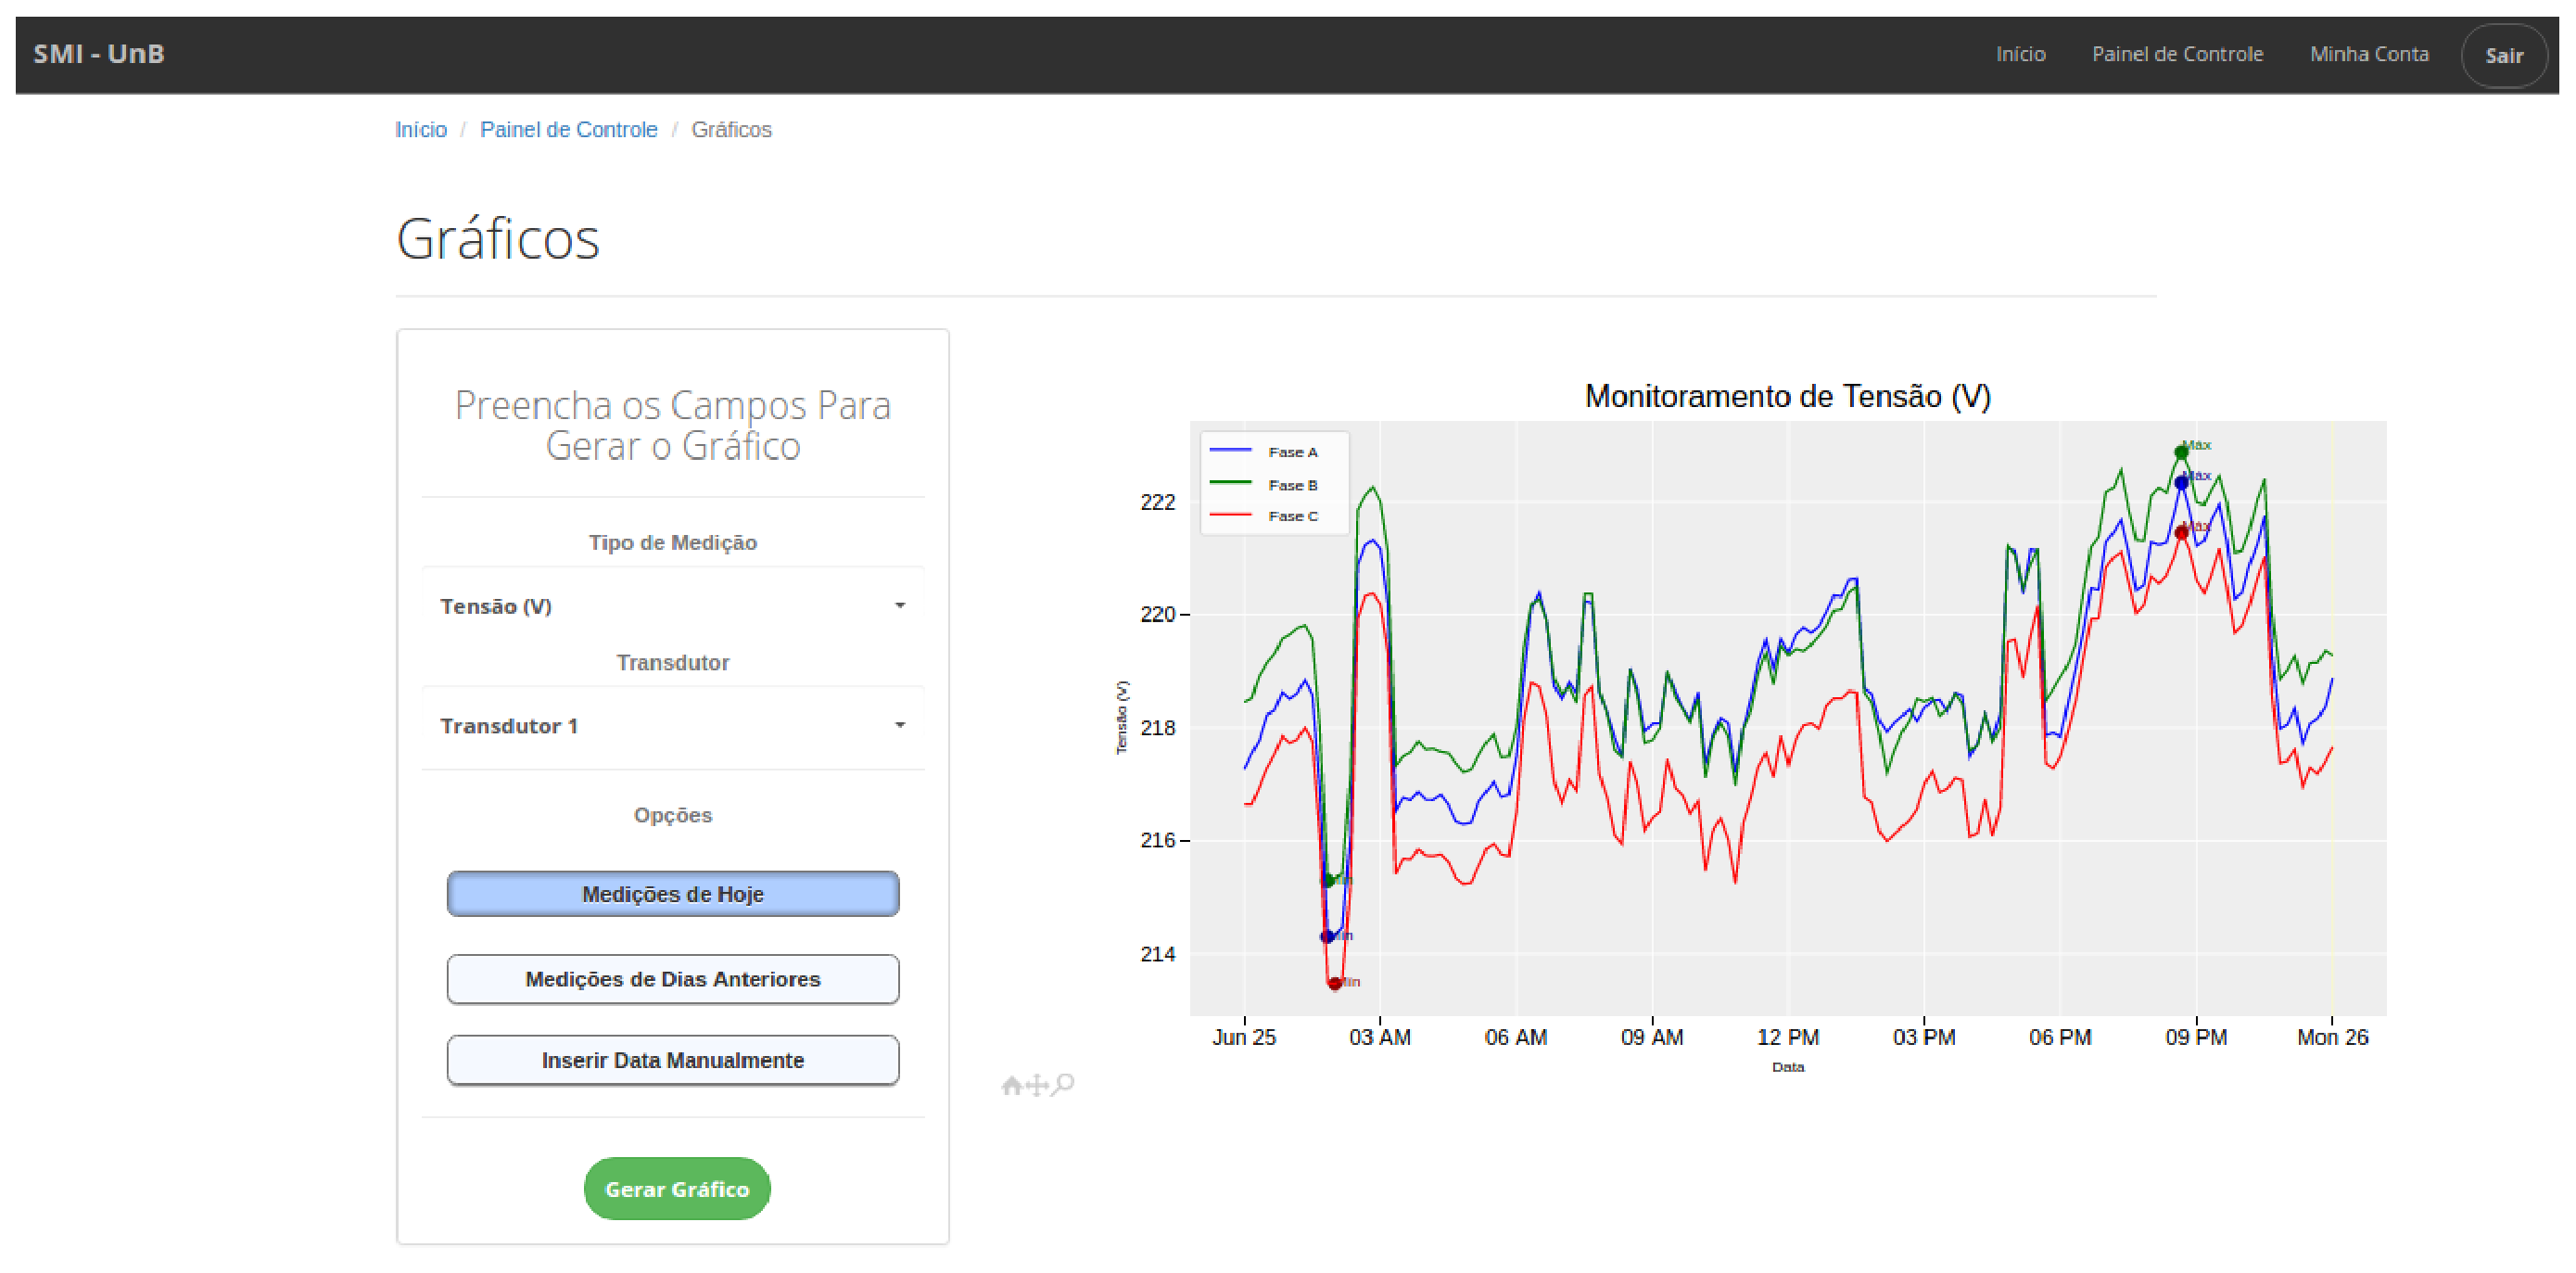
\includegraphics[keepaspectratio=true,scale=0.35]{figuras/img15.eps}
    \caption{Página de gráficos.}
    \label{img15}
\end{figure}

\begin{figure}[!htpb]
    \centering
    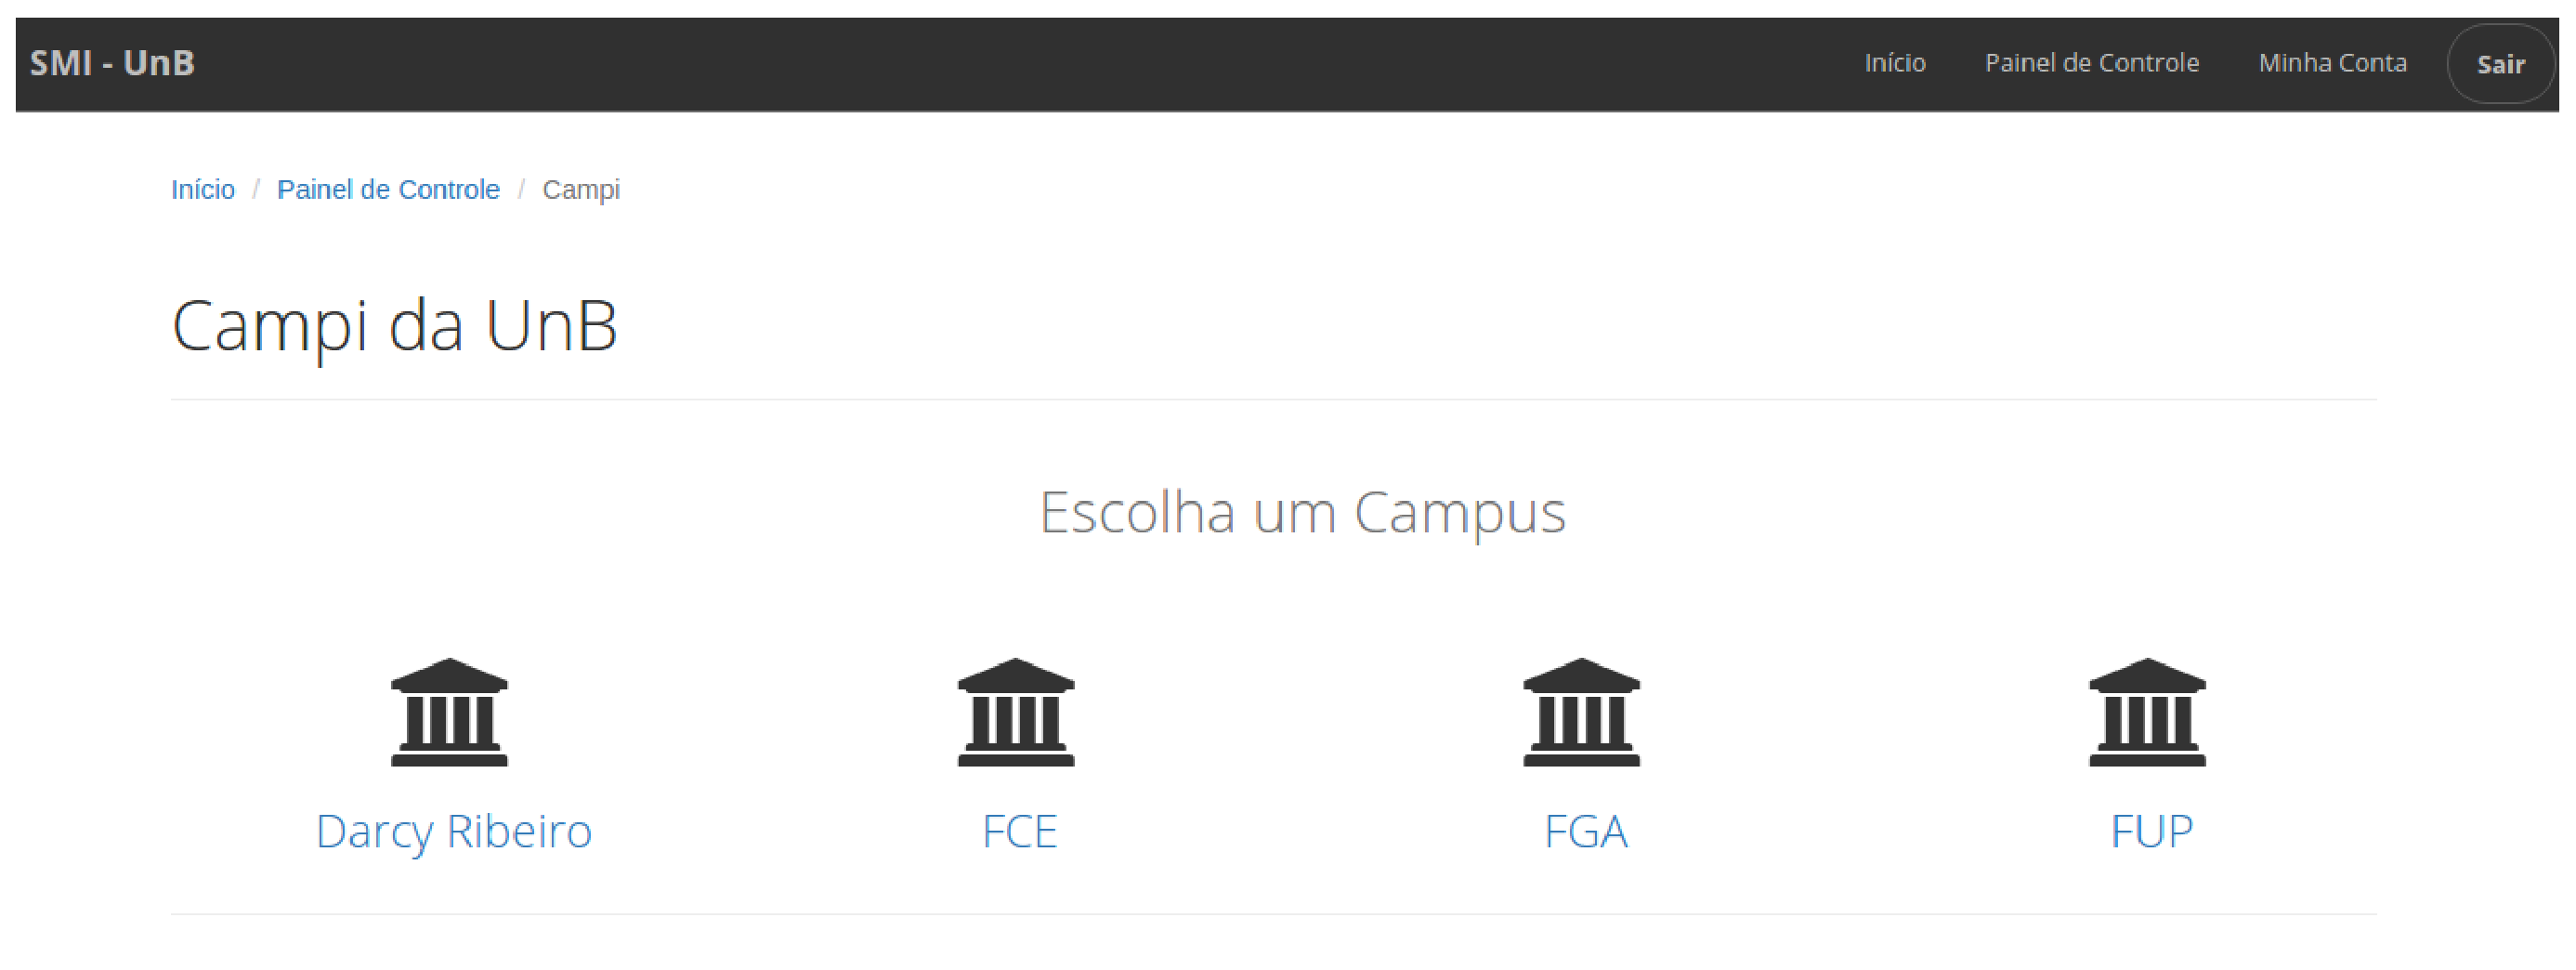
\includegraphics[keepaspectratio=true,scale=0.35]{figuras/img7.eps}
    \caption{Página dos \textit{campi} da UnB.}
    \label{img7}
\end{figure}

\begin{figure}[!htpb]
    \centering
    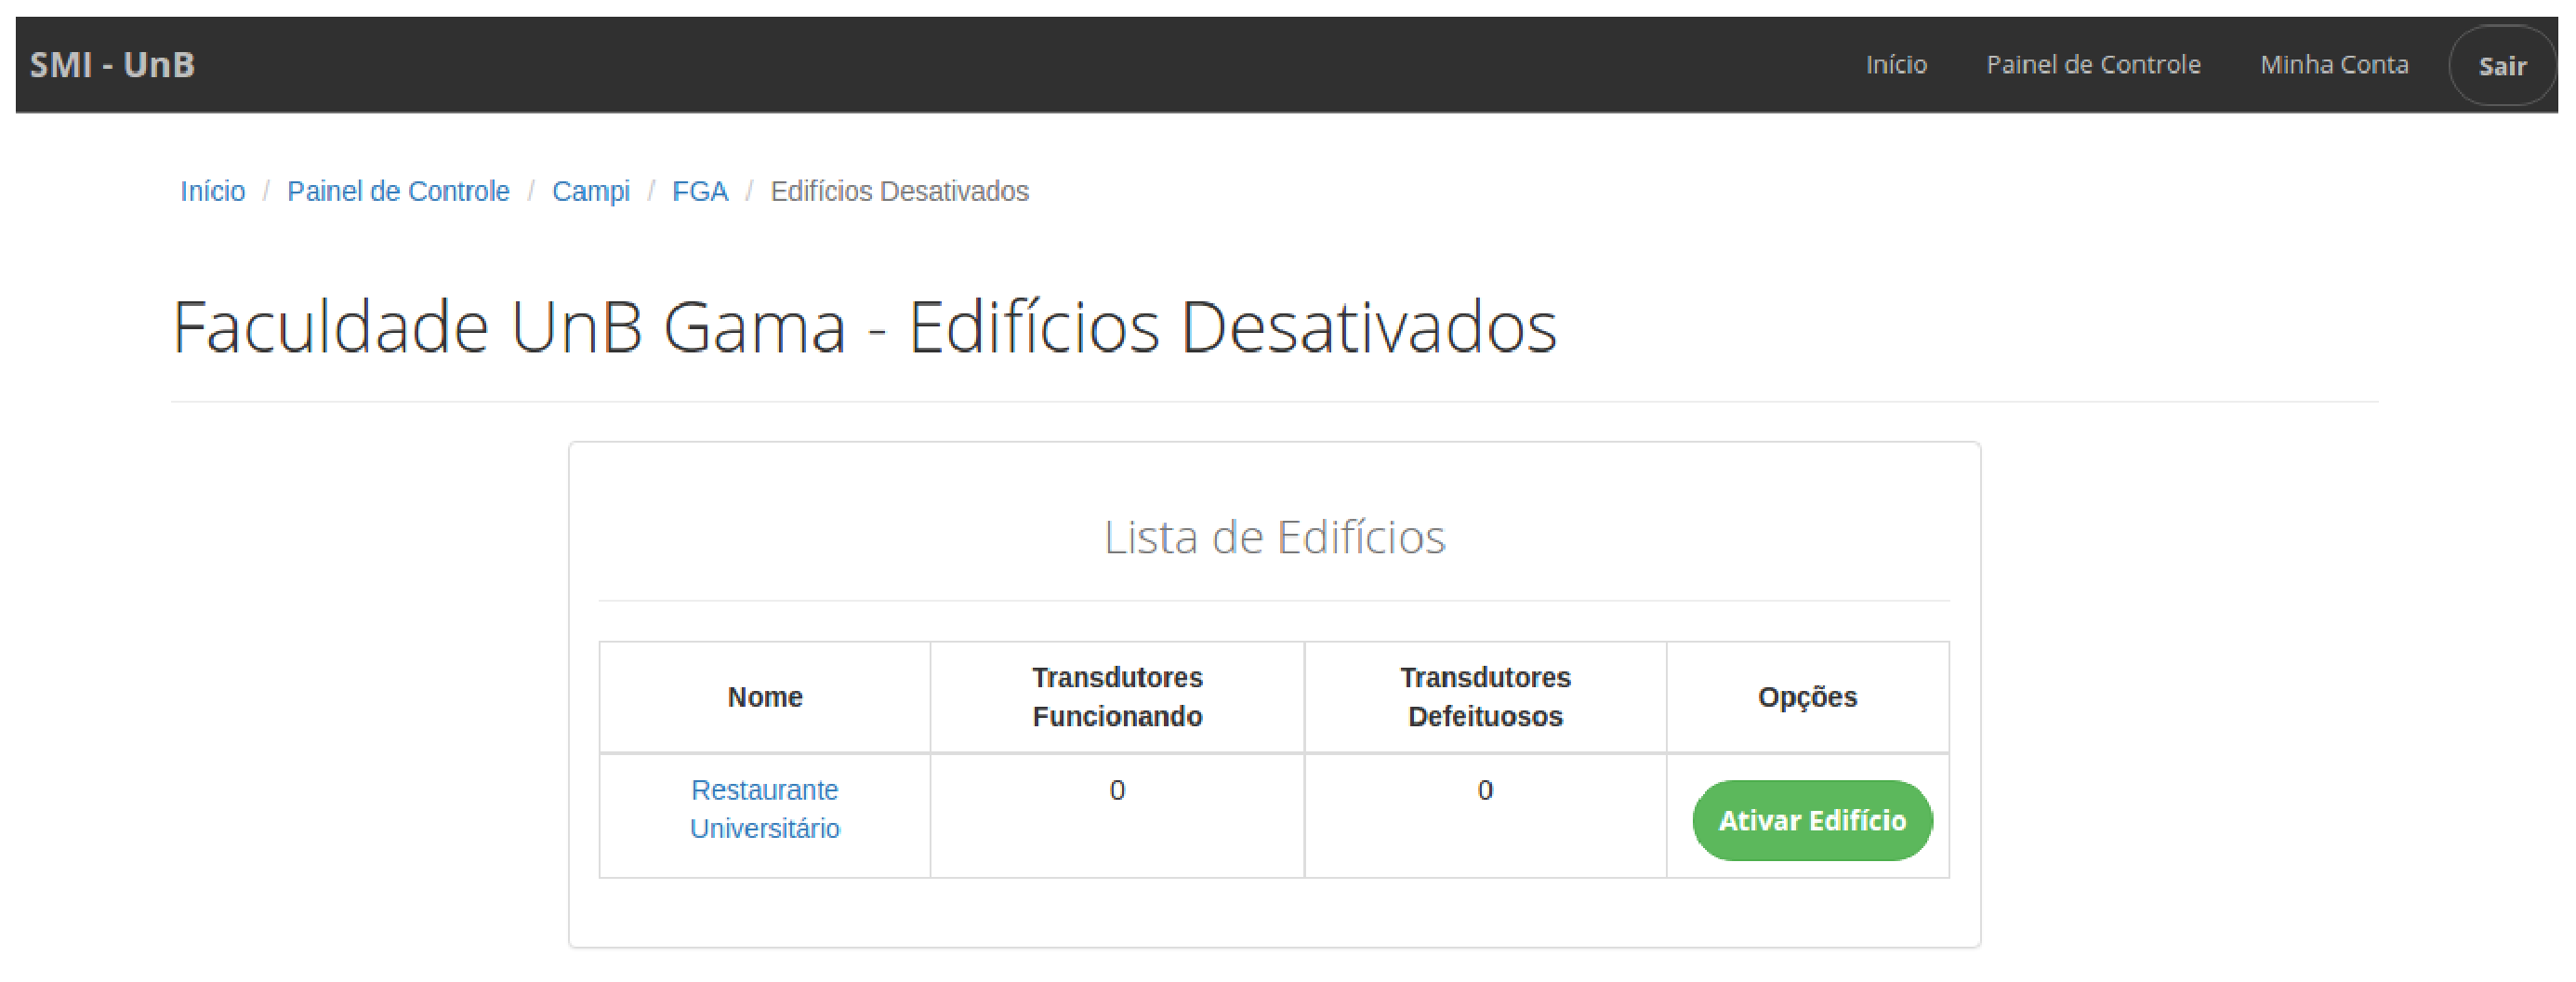
\includegraphics[keepaspectratio=true,scale=0.35]{figuras/img8.eps}
    \caption{Página de edifícios desativados em um campus.}
    \label{img8}
\end{figure}

\begin{figure}[!htpb]
    \centering
    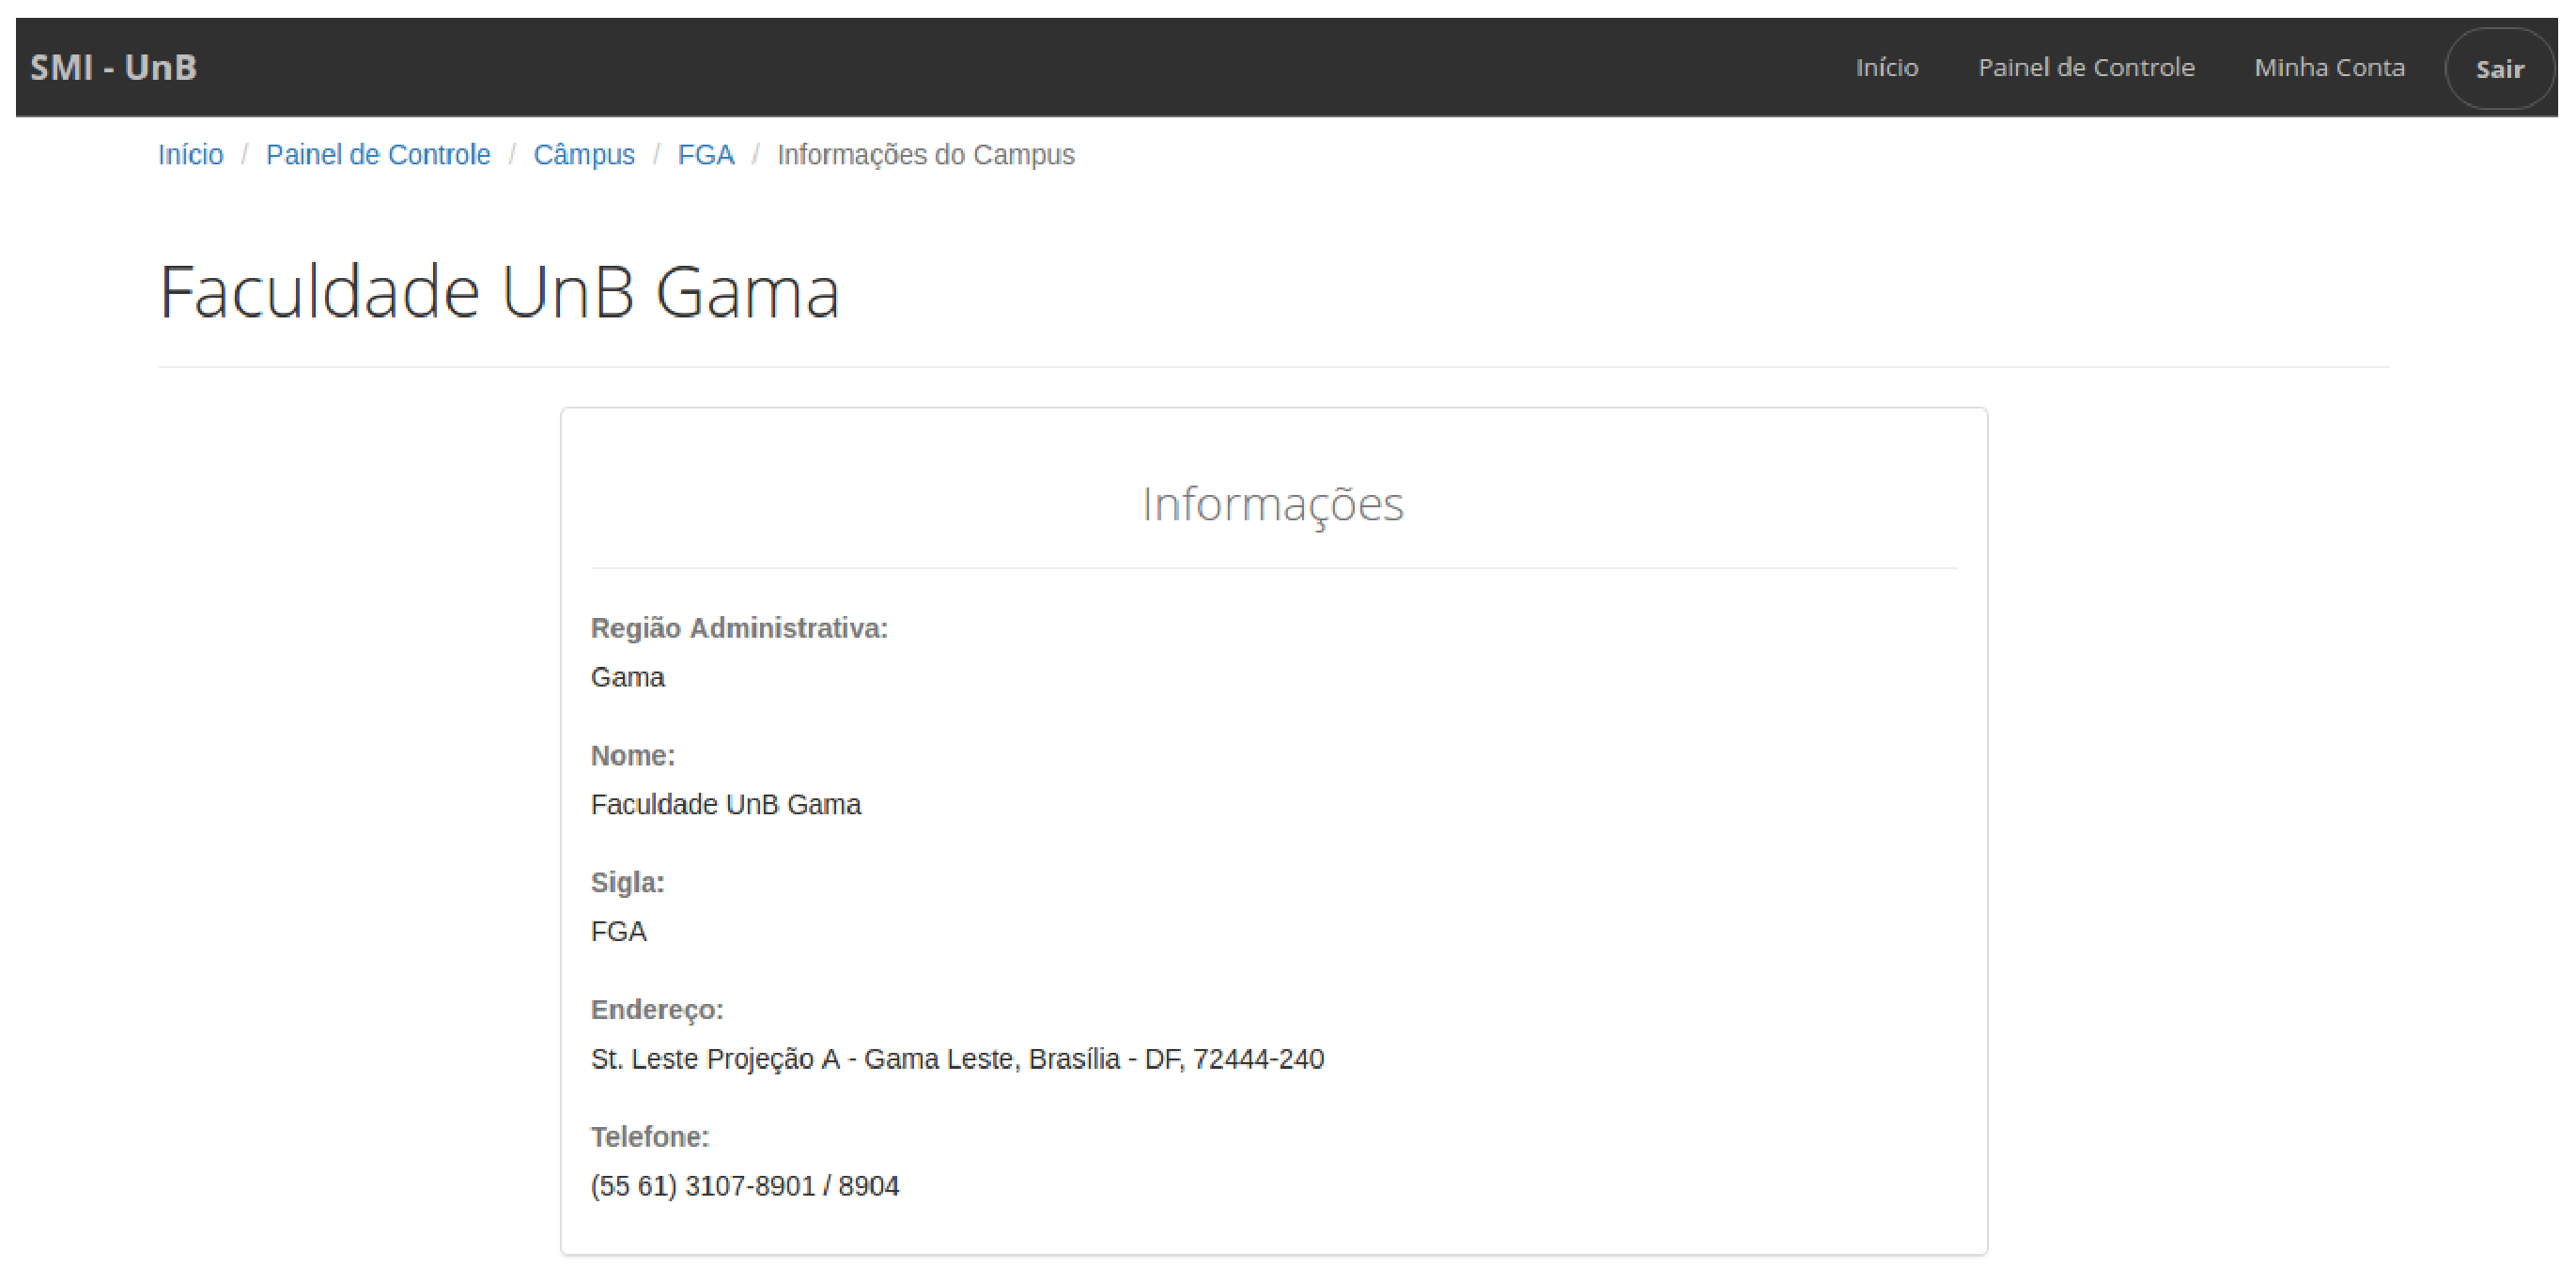
\includegraphics[keepaspectratio=true,scale=0.35]{figuras/img9.eps}
    \caption{Página de informações de em um campus.}
    \label{img9}
\end{figure}

\begin{figure}[!htpb]
    \centering
    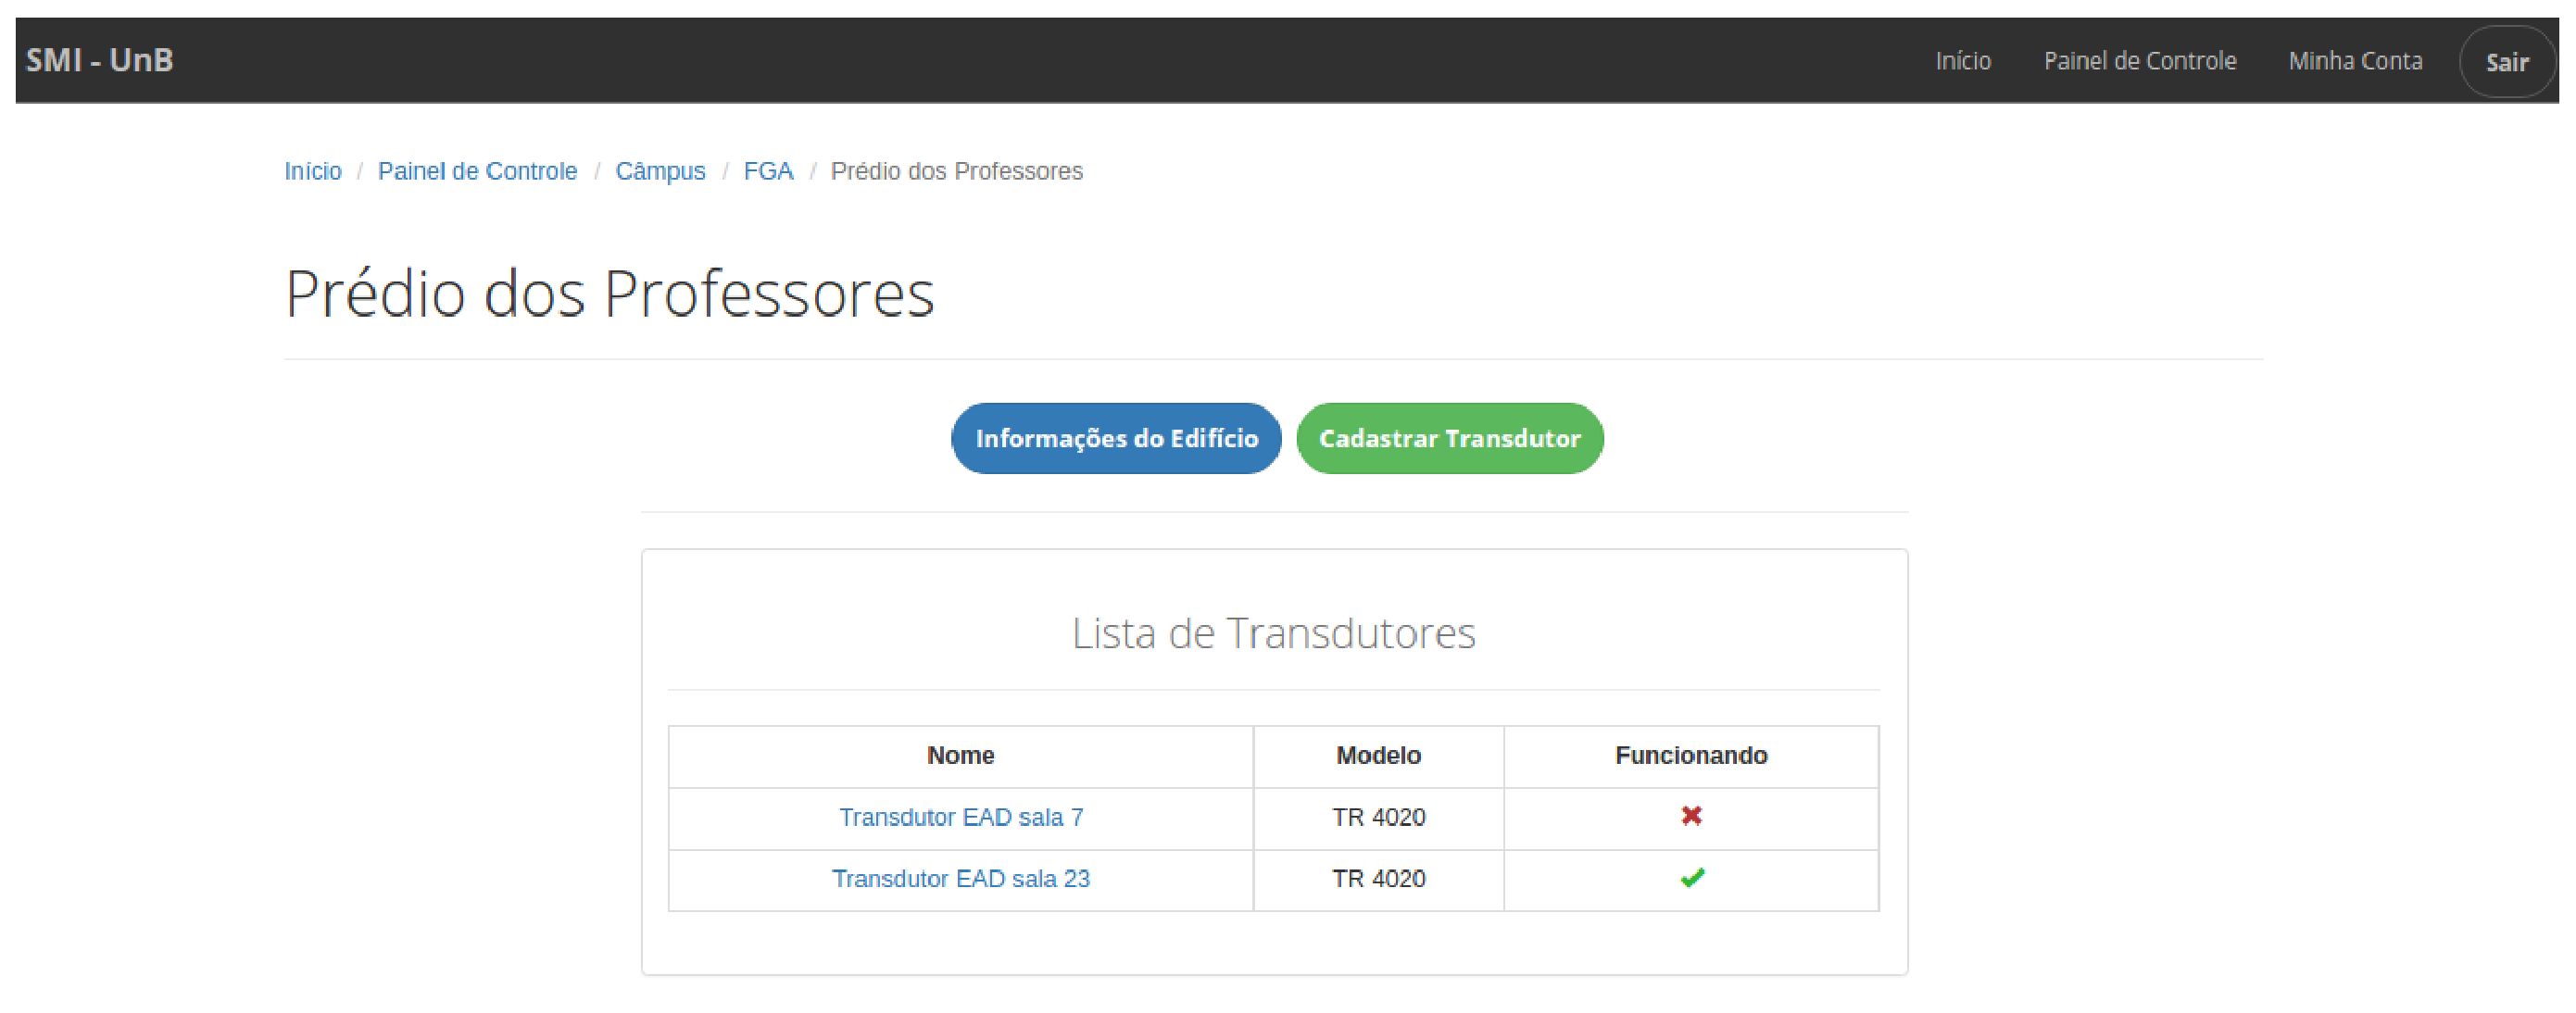
\includegraphics[keepaspectratio=true,scale=0.35]{figuras/img11.eps}
    \caption{Página principal de um edifício.}
    \label{img11}
\end{figure}

\begin{figure}[!htpb]
    \centering
    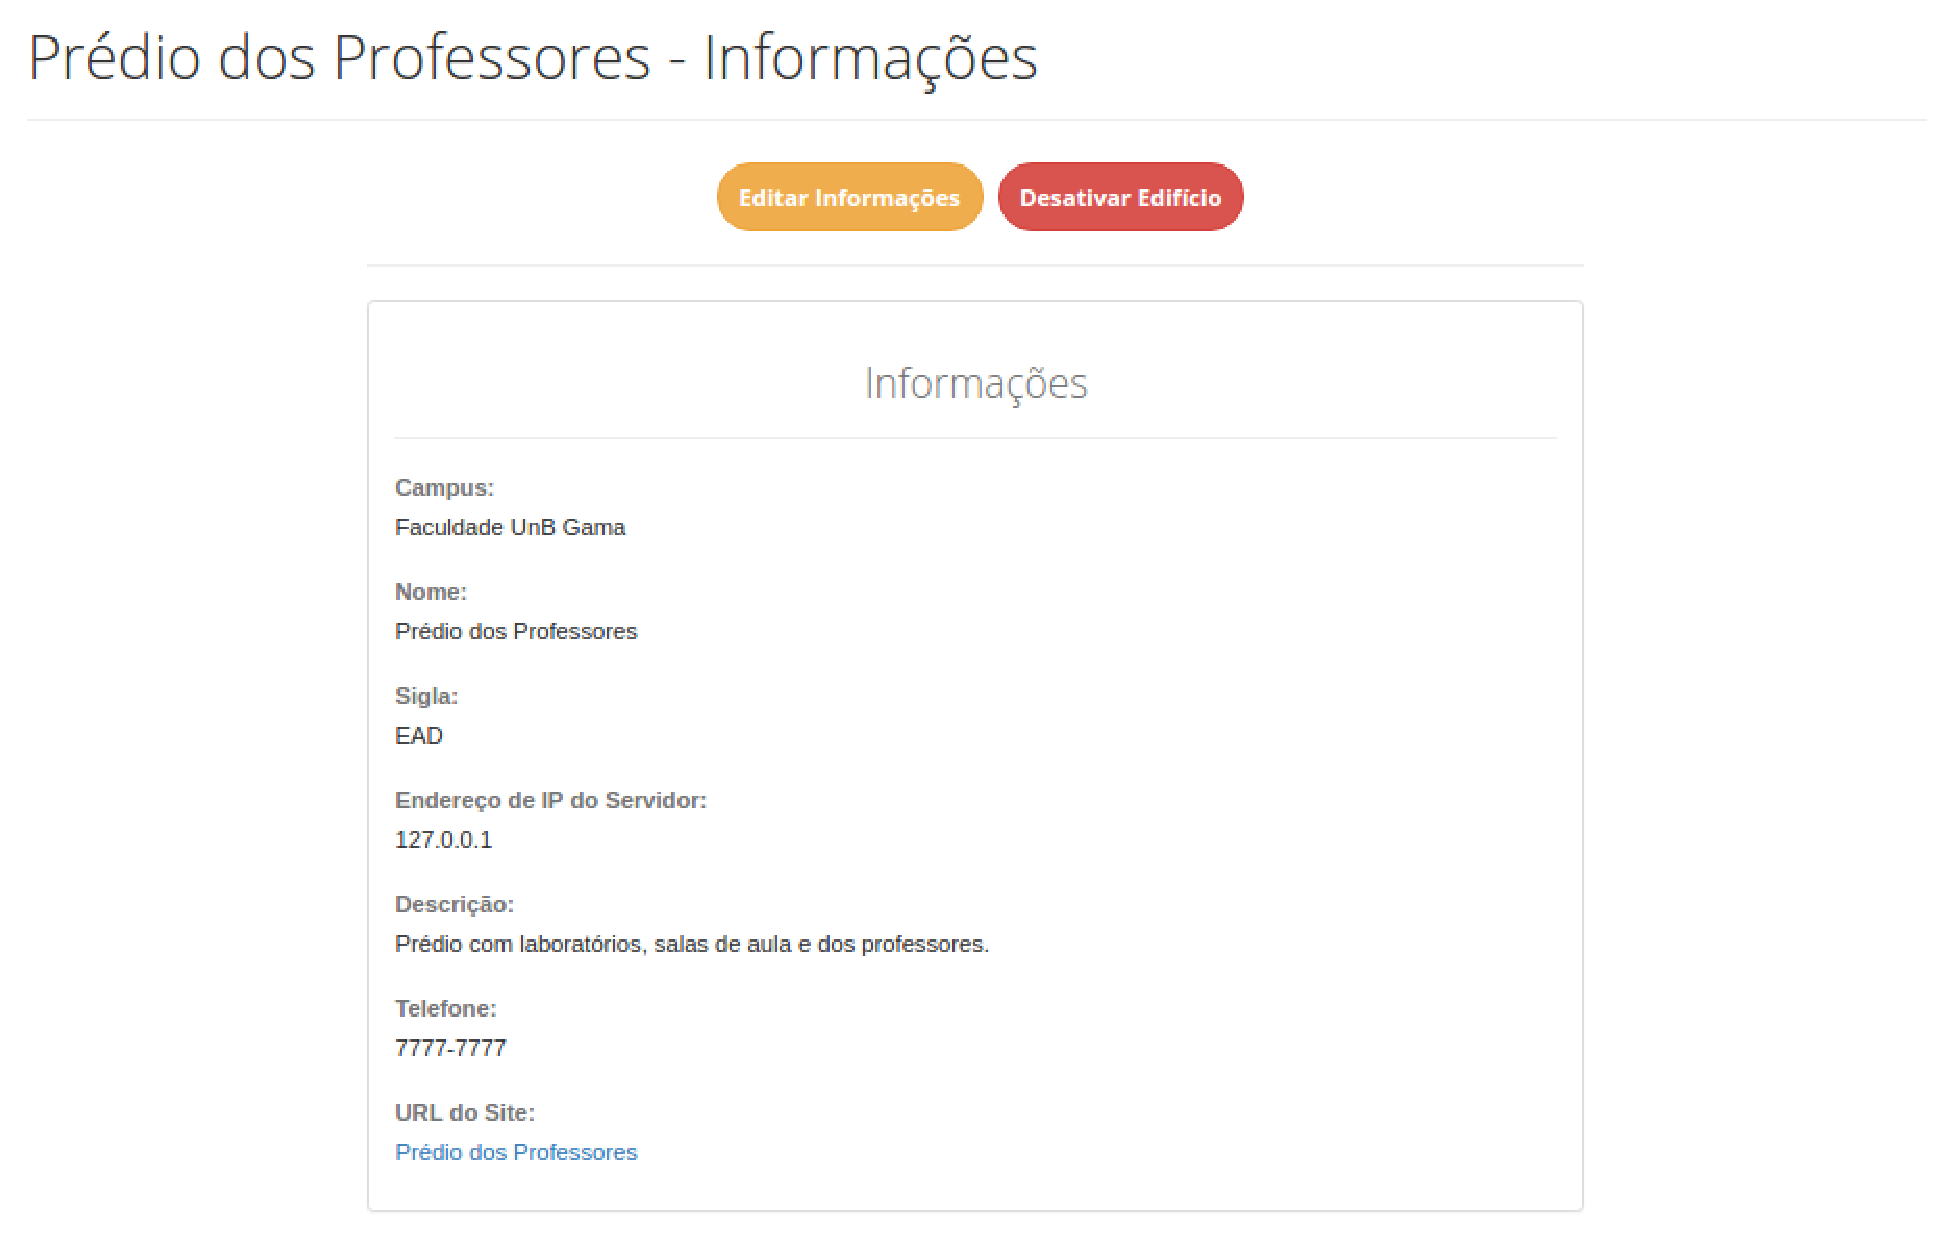
\includegraphics[keepaspectratio=true,scale=0.55]{figuras/img12.eps}
    \caption{Informações de um edifício.}
    \label{img12}
\end{figure}

\begin{figure}[!htpb]
    \centering
    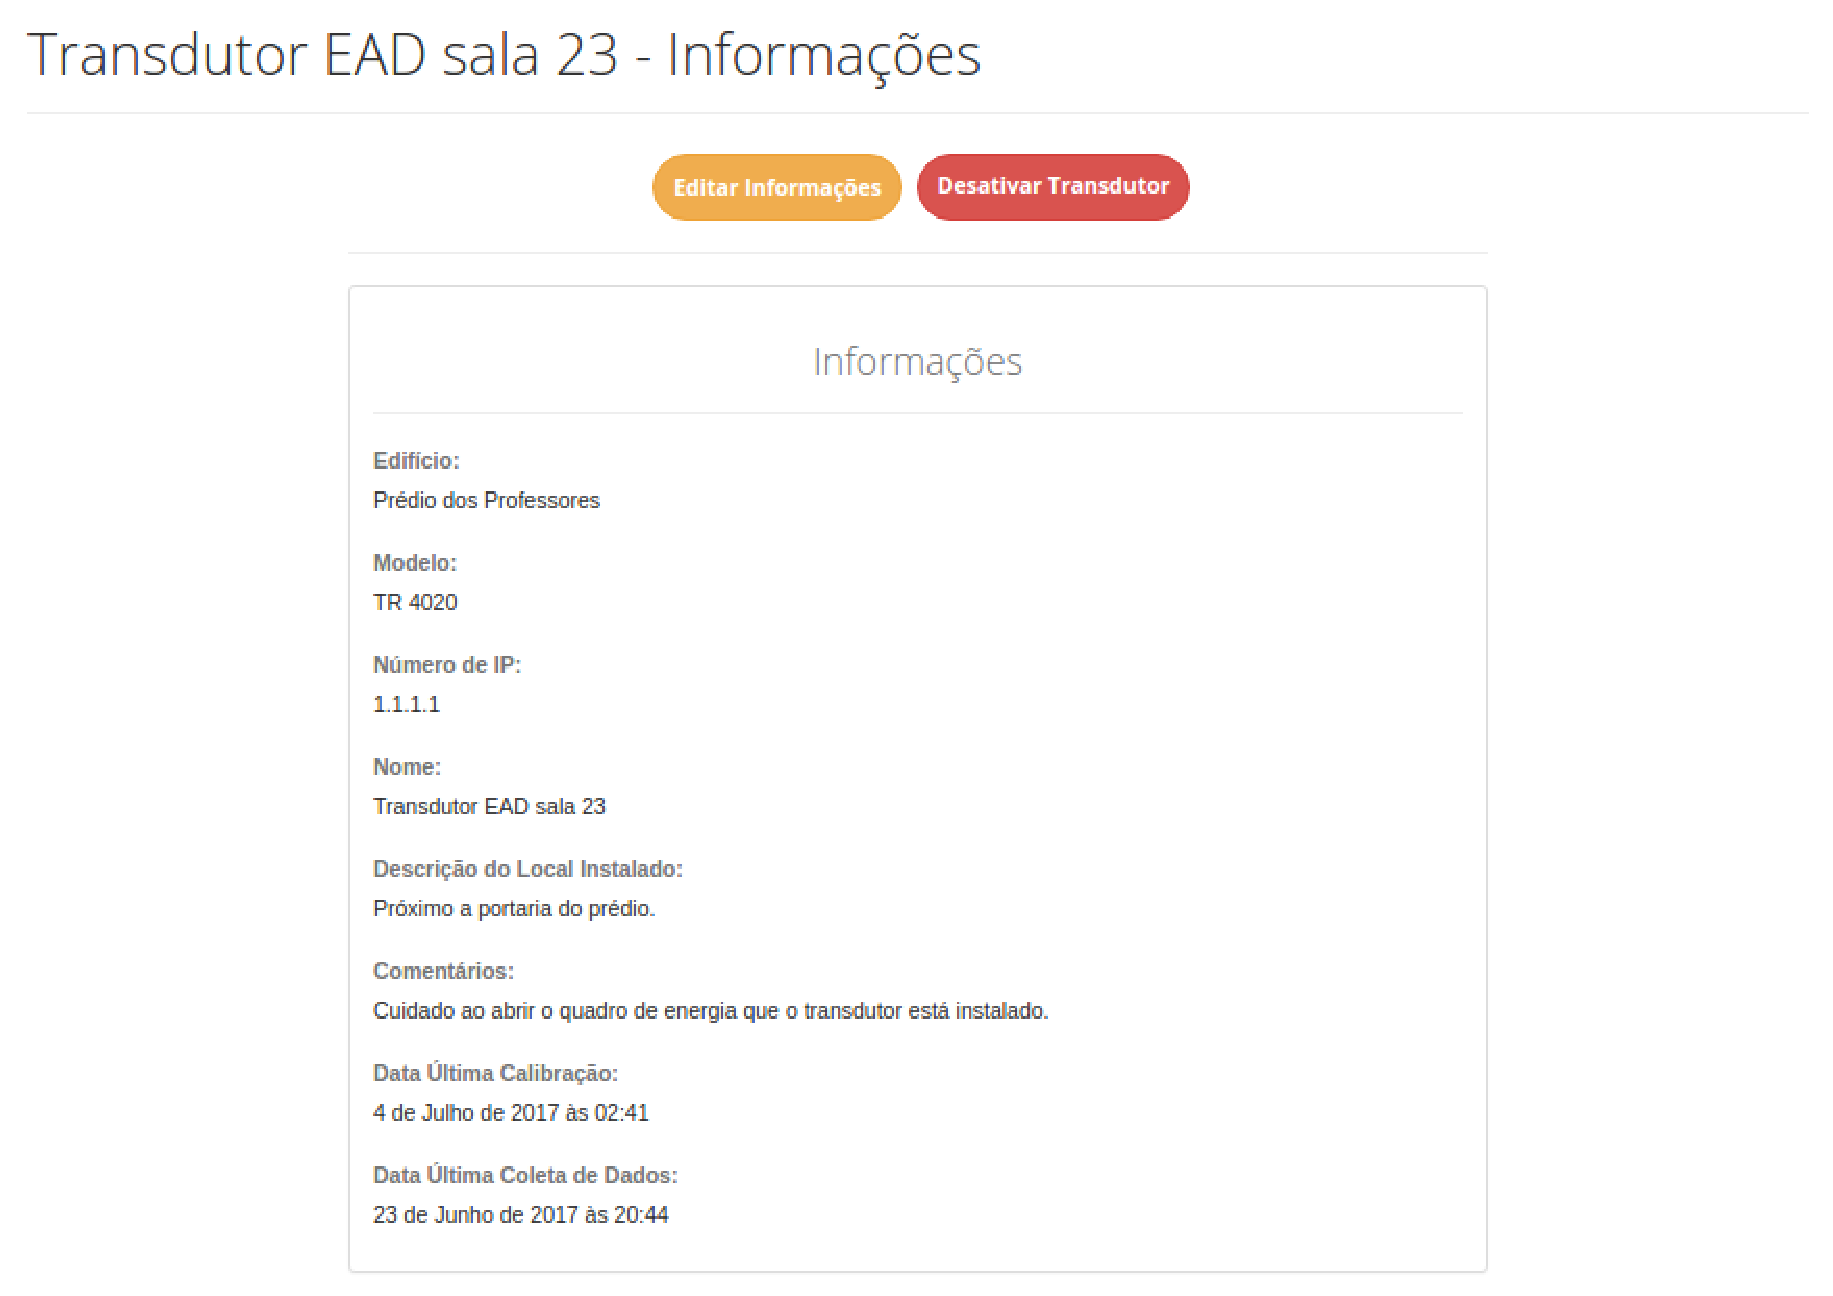
\includegraphics[keepaspectratio=true,scale=0.6]{figuras/img13.eps}
    \caption{Informações de um transdutor.}
    \label{img13}
\end{figure}

\begin{figure}[!htpb]
    \centering
    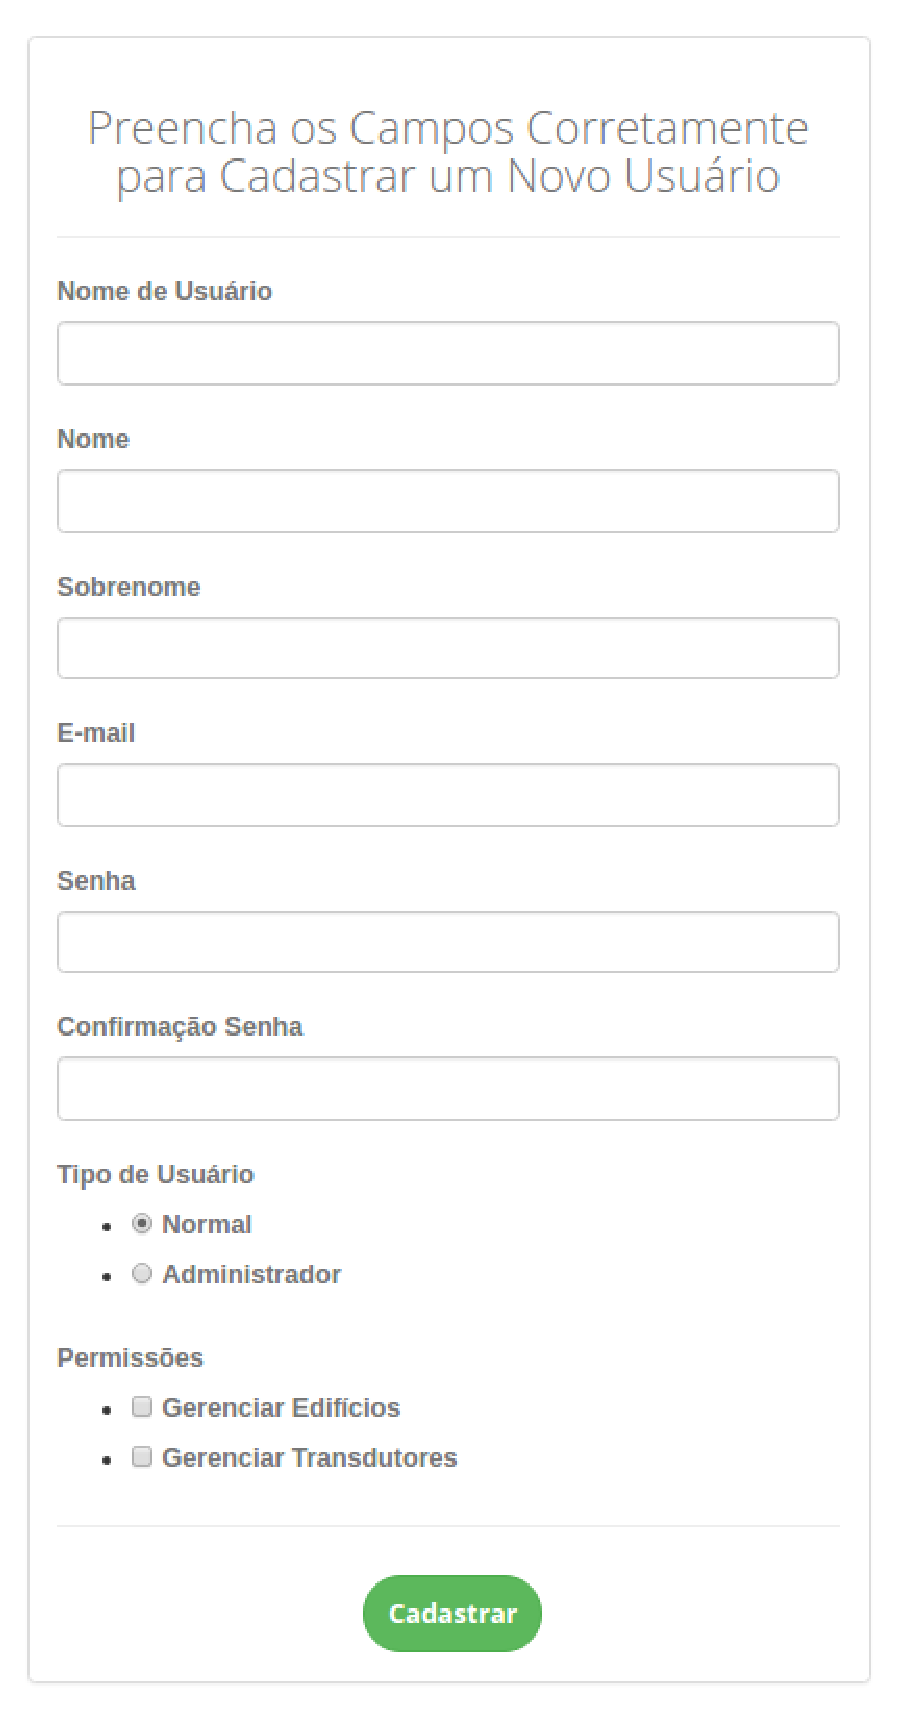
\includegraphics[keepaspectratio=true,scale=0.8]{figuras/img3.eps}
    \caption{Formulário para cadastro de um usuário.}
    \label{img3}
\end{figure}

\begin{figure}[!htpb]
    \centering
    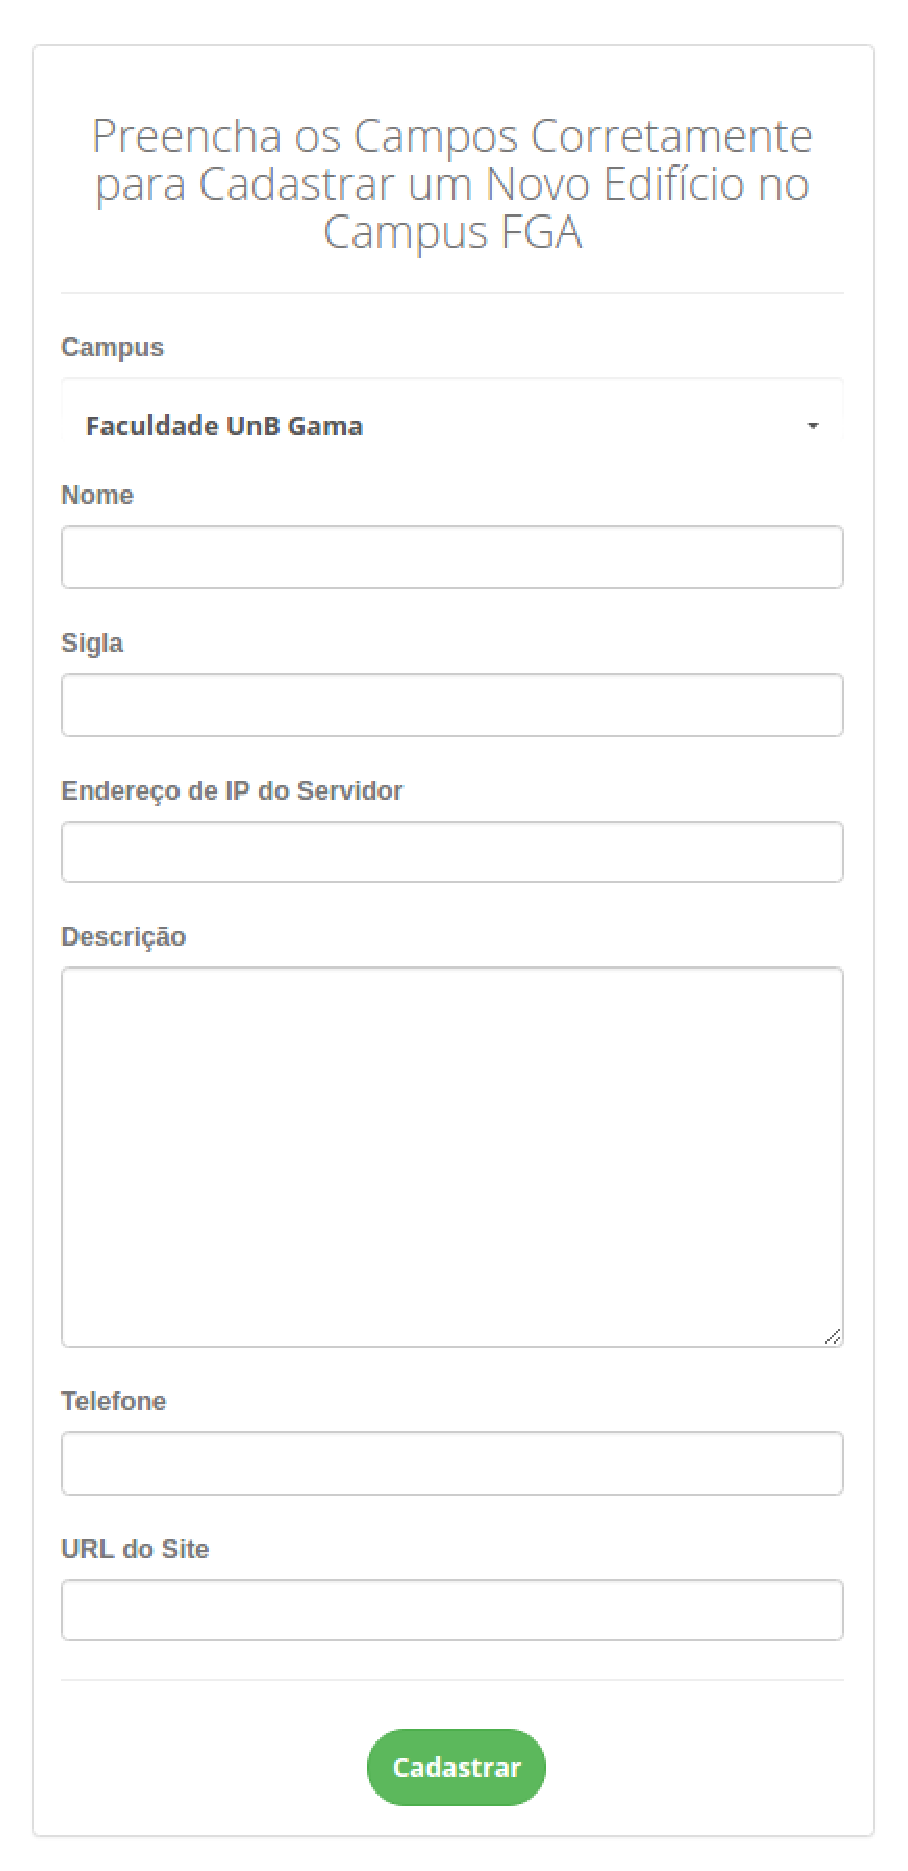
\includegraphics[keepaspectratio=true,scale=0.65]{figuras/img10.eps}
    \caption{Formulário para cadastro de um edifício.}
    \label{img10}
\end{figure}

\begin{figure}[!htpb]
    \centering
    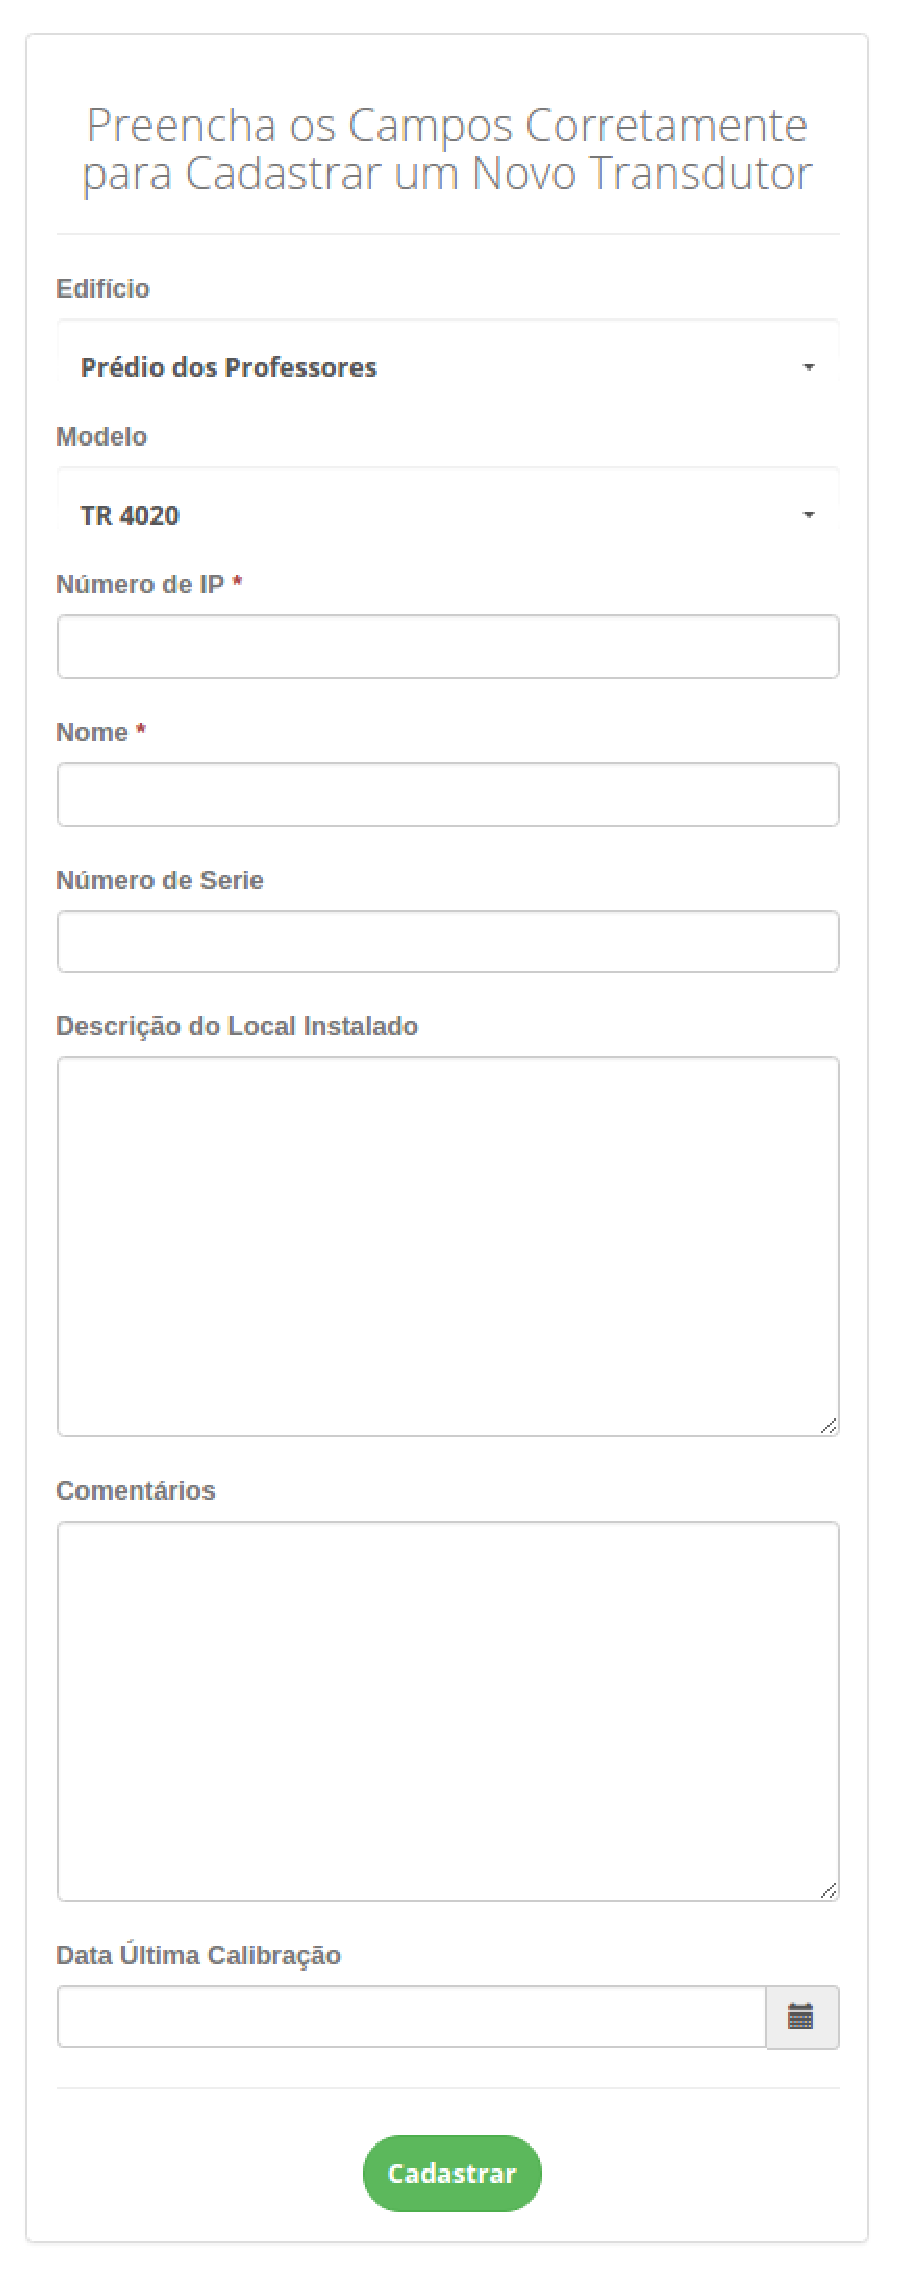
\includegraphics[keepaspectratio=true,scale=0.65]{figuras/img14.eps}
    \caption{Formulário para cadastro de um transdutor.}
    \label{img14}
\end{figure}

\end{apendicesenv}

\begin{anexosenv}

\partanexos

\end{anexosenv}
\printindex

\end{document}

